\chapter{Linear Second Order Equations}

\noindent
IN THIS CHAPTER we study a particularly important class of
second order equations.
Because of their many applications in science and engineering, second
order differential equation have historically been the most thoroughly
studied class of differential equations. Research on the theory of
second order differential equations continues to the present day. This
chapter is devoted to second order equations that can be written in
the form
$$
P_0(x)y''+P_1(x)y'+P_2(x)y=F(x).
$$
Such equations are said to be {\color{blue}\it linear\/}. As in the case of first
order linear equations, (A) is said to be {\color{blue}\it homogeneous\/}
if $F\equiv0$, or {\color{blue}\it nonhomogeneous\/} if $F\not\equiv0$.

\medskip\noindent
SECTION~5.1 is devoted to the theory of homogeneous linear
equations.

\medskip\noindent
 SECTION~5.2 deals with homogeneous equations of the
special form
$$
ay''+by'+cy=0,
$$
where $a$, $b$, and $c$ are constant ($a\ne0$). When you've
completed this section you'll know everything there is to know about
solving such equations.

\medskip\noindent
SECTION~5.3 presents the  theory of nonhomogeneous linear
equations.

\medskip\noindent
SECTIONS~5.4 AND 5.5
present  the {\color{blue}\it method of
undetermined coefficients\/}, which can be used to solve
nonhomogeneous equations of the form
$$
ay''+by'+cy=F(x),
$$
where $a$, $b$, and $c$ are constants and $F$ has a special form that
is still sufficiently general to occur in many applications. In this
section  we make extensive use of the idea of variation of
parameters
introduced in Chapter~2.

\medskip\noindent
SECTION~5.6  deals with {\color{blue}\it reduction of order\/}, a
technique based on the idea of variation of parameters,  which
enables us to find the general solution of a nonhomogeneous
linear second order equation provided that we know one nontrivial
(not identically zero) solution of the associated homogeneous
equation.

\medskip\noindent
SECTION~5.6
deals with the method traditionally called
{\color{blue}\it variation of parameters\/},
which enables us to find the general solution of a nonhomogeneous
linear second order equation provided that we know two nontrivial
solutions (with nonconstant ratio)  of the associated homogeneous
equation.

\newpage

\section{Homogeneous Linear Equations}

\noindent
A second order differential equation is said to be {\color{blue}\it linear\/} if it can be written
as
\begin{equation}
  \label{eq:5.1.1}y''+p(x)y'+q(x)y=f(x).
\end{equation}
We call the function $f$ on the right a {\color{blue}\it forcing function\/}, since in physical
applications it's often related to a force acting on some system modeled by the differential
equation. We say that \eqref{eq:5.1.1} is {\color{blue}\it homogeneous\/} if $f\equiv0$ or
{\color{blue}\it nonhomogeneous\/} if $f\not\equiv0$. Since these definitions are like the
corresponding definitions in Section~2.1 for the linear first order equation
\begin{equation}
  \label{eq:5.1.2}y'+p(x)y=f(x),
\end{equation}
it's natural to expect similarities between methods of solving \eqref{eq:5.1.1} and
\eqref{eq:5.1.2}. However, solving \eqref{eq:5.1.1} is more difficult than solving \eqref{eq:5.1.2}.
For example, while Theorem~\ref{thmtype:2.1.1} gives a formula for the general solution of
\eqref{eq:5.1.2} in the case where $f\equiv0$ and Theorem~\ref{thmtype:2.1.2} gives a formula for
the case where $f\not\equiv0$, there are no formulas for the general solution of \eqref{eq:5.1.1} in
either case. Therefore we must be content to solve linear second order equations of special forms.

In Section~2.1 we considered the homogeneous equation $y'+p(x)y=0$ first, and then used a nontrivial
solution of this equation to find the general solution of the nonhomogeneous equation
$y'+p(x)y=f(x)$. Although the progression from the homogeneous to the nonhomogeneous case isn't that
simple for the linear second order equation, it's still necessary to solve the homogeneous equation
\begin{equation}
  \label{eq:5.1.3}y''+p(x)y'+q(x)y=0
\end{equation}
in order to solve the nonhomogeneous equation \eqref{eq:5.1.1}. This section is devoted to
\eqref{eq:5.1.3}.

The next theorem gives sufficient conditions for existence and uniqueness of solutions of initial
value problems for \eqref{eq:5.1.3}. We omit the proof.

\begin{theorem}
  \color{blue}
  \label{thmtype:5.1.1} Suppose $p$ and $q$ are continuous on an open interval $(a,b)$, let $x_{0}$
  be any point in $(a,b)$, and let $k_{0}$ and $k_{1}$ be arbitrary real numbers. Then the initial
  value problem
  \[
    y''+p(x)y'+q(x)y=0,\ y(x_{0})=k_{0},\ y'(x_{0})=k_{1}
  \]
  has a unique solution on $(a,b)$.
\end{theorem}

Since $y\equiv0$ is obviously a solution of \eqref{eq:5.1.3} we call it the {\color{blue}\it
trivial} solution. Any other solution is {\color{blue}\it nontrivial}. Under the assumptions of
Theorem~\ref{thmtype:5.1.1}, the only solution of the initial value problem
\[
  y''+p(x)y'+q(x)y=0,\ y(x_{0})=0,\ y'(x_{0})=0
\]
on $(a,b)$ is the trivial solution (Exercise~\ref{exer:5.1.24}).

The next three examples illustrate concepts that we'll develop later in this section. You shouldn't
be concerned with how to {\color{blue}\it find\/} the given solutions of the equations in these
examples. This will be explained in later sections.

\begin{example}
  \label{example:5.1.1} \rm The coefficients of $y'$ and $y$ in
  \begin{equation}
    \label{eq:5.1.4}y''-y=0
  \end{equation}
  are the constant functions $p\equiv0$ and $q\equiv-1$, which are continuous on $(-\infty,\infty)$.
  Therefore Theorem~\ref{thmtype:5.1.1} implies that every initial value problem for
  \eqref{eq:5.1.4} has a unique solution on $(-\infty,\infty)$.
  \begin{alist}
    \item % (a)
    Verify that $y_{1}=e^{x}$ and $y_{2}=e^{-x}$ are solutions of \eqref{eq:5.1.4} on
    $(-\infty,\infty)$.

    \item % (b)
    Verify that if $c_{1}$ and $c_{2}$ are arbitrary constants, $y=c_{1}e^{x}+c_{2}e^{-x}$ is a
    solution of \eqref{eq:5.1.4} on $(-\infty,\infty)$.

    \item % (c)
    Solve the initial value problem
    \begin{equation}
      \label{eq:5.1.5}y''-y=0,\quad y(0)=1,\quad y'(0)=3.
    \end{equation}
  \end{alist}
\end{example}

\solutionpart{a} If $y_{1}=e^{x}$ then $y_{1}'=e^{x}$ and $y_{1}''=e^{x}=y_{1}$, so
$y_{1}''-y_{1}=0$. If $y_{2}=e^{-x}$, then $y_{2}'=-e^{-x}$ and $y_{2}''=e^{-x}=y_{2}$, so
$y_{2}''-y_{2}=0$.

\solutionpart{b} If
\begin{equation}
  \label{eq:5.1.6}y=c_{1}e^{x}+c_{2}e^{-x}
\end{equation}
then
\begin{equation}
  \label{eq:5.1.7}y'=c_{1}e^{x}-c_{2}e^{-x}
\end{equation}
and
\[
  y''=c_{1}e^{x}+c_{2}e^{-x},
\]
so
\begin{eqnarray*}
  y''-y & = & (c_{1}e^{x}+c_{2}e^{-x})-(c_{1}e^{x}+c_{2}e^{-x}) \\
        & = & c_{1}(e^{x}-e^{x})+c_{2}(e^{-x}-e^{-x})=0
\end{eqnarray*}
for all $x$. Therefore $y=c_{1}e^{x}+c_{2}e^{-x}$ is a solution of \eqref{eq:5.1.4} on
$(-\infty,\infty)$.

\solutionpart{c} We can solve \eqref{eq:5.1.5} by choosing $c_{1}$ and $c_{2}$ in \eqref{eq:5.1.6}
so that $y(0)=1$ and $y'(0)=3$. Setting $x=0$ in \eqref{eq:5.1.6} and \eqref{eq:5.1.7} shows that
this is equivalent to
\begin{eqnarray*}
  c_{1}+c_{2} & = & 1 \\
  c_{1}-c_{2} & = & 3.
\end{eqnarray*}
Solving these equations yields $c_{1}=2$ and $c_{2}=-1$. Therefore $y=2e^{x}-e^{-x}$ is the unique
solution of \eqref{eq:5.1.5} on $(-\infty,\infty)$.

\begin{example}
  \label{example:5.1.2} \rm %\newcommand{\exampletrig}
  Let $\omega$ be a positive constant. The coefficients of $y'$ and $y$ in
  \begin{equation}
    \label{eq:5.1.8}y''+\omega^{2}y=0
  \end{equation}
  are the constant functions $p\equiv0$ and $q\equiv\omega^{2}$, which are continuous on
  $(-\infty,\infty)$. Therefore Theorem~\ref{thmtype:5.1.1} implies that every initial value problem
  for \eqref{eq:5.1.8} has a unique solution on $(-\infty,\infty)$.
  \begin{alist}
    \item % (a)
    Verify that $y_{1}=\cos\omega x$ and $y_{2}=\sin\omega x$ are solutions of \eqref{eq:5.1.8} on
    $(-\infty,\infty)$.

    \item % (b)
    Verify that if $c_{1}$ and $c_{2}$ are arbitrary constants then
    $y=c_{1}\cos\omega x+c_{2}\sin\omega x$ is a solution of \eqref{eq:5.1.8} on $(-\infty,\infty)$.

    \item % (c)
    Solve the initial value problem
    \begin{equation}
      \label{eq:5.1.9}y''+\omega^{2}y=0,\quad y(0)=1,\quad y'(0)=3.
    \end{equation}
  \end{alist}
\end{example}

\solutionpart{a} If $y_{1}=\cos\omega x$ then $y_{1}'=-\omega\sin\omega x$ and
$y_{1}''=-\omega^{2}\cos\omega x=-\omega^{2}y_{1}$, so $y_{1}''+\omega^{2}y_{1}=0$. If
$y_{2}=\sin\omega x$ then, $y_{2}'=\omega\cos\omega x$ and
$y_{2}''=-\omega^{2}\sin\omega x=-\omega^{2}y_{2}$, so $y_{2}''+\omega^{2}y_{2}=0$.

\solutionpart{b} If
\begin{equation}
  \label{eq:5.1.10}y=c_{1}\cos\omega x+c_{2}\sin\omega x
\end{equation}
then
\begin{equation}
  \label{eq:5.1.11}y'=\omega(-c_{1}\sin\omega x+c_{2}\cos\omega x)
\end{equation}
and
\[
  y''=-\omega^{2}(c_{1}\cos\omega x+c_{2}\sin\omega x),
\]
so
\begin{eqnarray*}
  y''+\omega^{2}y & = & -\omega^{2}(c_{1}\cos\omega x+c_{2}\sin\omega x)+\omega^{2}(c_{1}\cos\omega x+c_{2}\sin\omega x) \\
                  & = & c_{1}\omega^{2}(-\cos\omega x+\cos\omega x)+c_{2}\omega^{2}(-\sin\omega x+\sin\omega x)=0
\end{eqnarray*}
for all $x$. Therefore $y=c_{1}\cos\omega x+c_{2}\sin\omega x$ is a solution of \eqref{eq:5.1.8} on
$(-\infty,\infty)$.

\solutionpart{c} To solve \eqref{eq:5.1.9}, we must choosing $c_{1}$ and $c_{2}$ in
\eqref{eq:5.1.10} so that $y(0)=1$ and $y'(0)=3$. Setting $x=0$ in \eqref{eq:5.1.10} and
\eqref{eq:5.1.11} shows that $c_{1}=1$ and $c_{2}=3/\omega$. Therefore
\[
  y=\cos\omega x+\frac{3}{\omega}\sin\omega x
\]
is the unique solution of \eqref{eq:5.1.9} on $(-\infty,\infty)$. \bbox

Theorem~\ref{thmtype:5.1.1} implies that if $k_{0}$ and $k_{1}$ are arbitrary real numbers then the
initial value problem
\begin{equation}
  \label{eq:5.1.12}P_{0}(x)y''+P_{1}(x)y'+P_{2}(x)y=0,\quad y(x_{0})=k_{0},\quad y'(x_{0})=k_{1}
\end{equation}
has a unique solution on an interval $(a,b)$ that contains $x_{0}$, provided that $P_{0}$, $P_{1}$,
and $P_{2}$ are continuous and $P_{0}$ has no zeros on $(a,b)$. To see this, we rewrite the
differential equation in \eqref{eq:5.1.12} as
\[
  y''+\frac{P_{1}(x)}{P_{0}(x)}y'+\frac{P_{2}(x)}{P_{0}(x)}y=0
\]
and apply Theorem~\ref{thmtype:5.1.1} with $p=P_{1}/P_{0}$ and $q=P_{2}/P_{0}$.

\begin{example}
  \label{example:5.1.3} \rm The equation
  \begin{equation}
    \label{eq:5.1.13}x^{2}y''+xy'-4y=0
  \end{equation}
  has the form of the differential equation in \eqref{eq:5.1.12}, with $P_{0}(x)=x^{2}$,
  $P_{1}(x)=x$, and $P_{2}(x)=-4$, which are all continuous on $(-\infty,\infty)$. However, since
  $P(0)=0$ we must consider solutions of \eqref{eq:5.1.13} on $(-\infty,0)$ and $(0,\infty)$. Since
  $P_{0}$ has no zeros on these intervals, Theorem~\ref{thmtype:5.1.1} implies that the initial
  value problem
  \[
    x^{2}y''+xy'-4y=0,\quad y(x_{0})=k_{0},\quad y'(x_{0})=k_{1}
  \]
  has a unique solution on $(0,\infty)$ if $x_{0}>0$, or on $(-\infty,0)$ if $x_{0}<0$.
  \begin{alist}
    \item % (a)
    Verify that $y_{1}=x^{2}$ is a solution of \eqref{eq:5.1.13} on $(-\infty,\infty)$ and
    $y_{2}=1/x^{2}$ is a solution of \eqref{eq:5.1.13} on $(-\infty,0)$ and $(0,\infty)$.

    \item % (b)
    Verify that if $c_{1}$ and $c_{2}$ are any constants then $y=c_{1}x^{2}+c_{2}/x^{2}$ is a
    solution of \eqref{eq:5.1.13} on $(-\infty,0)$ and $(0,\infty)$.

    \item % (c)
    Solve the initial value problem
    \begin{equation}
      \label{eq:5.1.14}x^{2}y''+xy'-4y=0,\quad y(1)=2,\quad y'(1)=0.
    \end{equation}

    \item % (d)
    Solve the initial value problem
    \begin{equation}
      \label{eq:5.1.15}x^{2}y''+xy'-4y=0,\quad y(-1)=2,\quad y'(-1)=0.
    \end{equation}
  \end{alist}
\end{example}

\solutionpart{a} If $y_{1}=x^{2}$ then $y_{1}'=2x$ and $y_{1}''=2$, so
\[
  x^{2}y_{1}''+xy_{1}'-4y_{1}=x^{2}(2)+x(2x)-4x^{2}=0
\]
for $x$ in $(-\infty,\infty)$. If $y_{2}=1/x^{2}$, then $y_{2}'=-2/x^{3}$ and $y_{2}''=6/x^{4}$, so
\[
  x^{2}y_{2}''+xy_{2}'-4y_{2}=x^{2}\left(\frac{6}{x^{4}}\right)-x\left(\frac{2}{x^{3}}\right)-\frac{4}{x^{2}}=0
\]
for $x$ in $(-\infty,0)$ or $(0,\infty)$.

\solutionpart{b} If
\begin{equation}
  \label{eq:5.1.16}y=c_{1}x^{2}+\frac{c_{2}}{x^{2}}
\end{equation}
then
\begin{equation}
  \label{eq:5.1.17}y'=2c_{1}x-\frac{2c_{2}}{x^{3}}
\end{equation}
and
\[
  y''=2c_{1}+\frac{6c_{2}}{x^{4}},
\]
so
\begin{eqnarray*}
  x^{2}y''+xy'-4y & = & x^{2}\dst{\left(2c_{1}+\frac{6c_{2}}{x^{4}}\right)}+x\dst{\left(2c_{1}x-\frac{2c_{2}}{x^{3}}\right)}-4\dst{\left(c_{1}x^{2}+\frac{c_{2}}{x^{2}}\right)} \\[2\jot]
                  & = & c_{1}(2x^{2}+2x^{2}-4x^{2})+c_{2}\dst{\left(\frac{6}{x^{2}}-\frac{2}{x^{2}}-\frac{4}{x^{2}}\right)}                                                     \\[2\jot]
                  & = & c_{1}\cdot0+c_{2}\cdot0=0
\end{eqnarray*}
for $x$ in $(-\infty,0)$ or $(0,\infty)$.

\solutionpart{c} To solve \eqref{eq:5.1.14}, we choose $c_{1}$ and $c_{2}$ in \eqref{eq:5.1.16} so
that $y(1)=2$ and $y'(1)=0$. Setting $x=1$ in \eqref{eq:5.1.16} and \eqref{eq:5.1.17} shows that
this is equivalent to
\begin{eqnarray*}
  \phantom{2}c_{1}+\phantom{2}c_{2} & = & 2 \\
  2c_{1}-2c_{2}                     & = & 0.
\end{eqnarray*}
Solving these equations yields $c_{1}=1$ and $c_{2}=1$. Therefore $y=x^{2}+1/x^{2}$ is the unique
solution of \eqref{eq:5.1.14} on $(0,\infty)$.

\solutionpart{d} We can solve \eqref{eq:5.1.15} by choosing $c_{1}$ and $c_{2}$ in \eqref{eq:5.1.16}
so that $y(-1)=2$ and $y'(-1)=0$. Setting $x=-1$ in \eqref{eq:5.1.16} and \eqref{eq:5.1.17} shows
that this is equivalent to
\begin{eqnarray*}
  \phantom{-2}c_{1}+\phantom{2}c_{2} & = & 2 \\
  -2c_{1}+2c_{2}                     & = & 0.
\end{eqnarray*}
Solving these equations yields $c_{1}=1$ and $c_{2}=1$. Therefore $y=x^{2}+1/x^{2}$ is the unique
solution of \eqref{eq:5.1.15} on $(-\infty,0)$. \bbox

Although the {\color{blue}\it formulas\/} for the solutions of \eqref{eq:5.1.14} and
\eqref{eq:5.1.15} are both $y=x^{2}+1/x^{2}$, you should not conclude that these two initial value
problems have the same solution. Remember that a solution of an initial value problem is defined
{\color{blue}\it on an interval that contains the initial point\/}; therefore, the solution of
\eqref{eq:5.1.14} is $y=x^{2}+1/x^{2}$ {\color{blue}\it on the interval\/} $(0,\infty)$, which
contains the initial point $x_{0}=1$, while the solution of \eqref{eq:5.1.15} is $y=x^{2}+1/x^{2}$
{\color{blue}\it on the interval\/} $(-\infty,0)$, which contains the initial point $x_{0}=-1$.

\boxit{The General Solution of a Homogeneous Linear Second Order Equation}

\noindent
If $y_{1}$ and $y_{2}$ are defined on an interval $(a,b)$ and $c_{1}$ and $c_{2}$ are constants,
then
\[
  y=c_{1}y_{1}+c_{2}y_{2}
\]
is a {\color{blue}\it linear combination of $y_{1}$ and $y_{2}$\/}. For example, $y=2\cos x+7\sin x$
is a linear combination of $y_{1}= \cos x$ and $y_{2}=\sin x$, with $c_{1}=2$ and $c_{2}=7$.

The next theorem states a fact that we've already verified in Examples~\ref{example:5.1.1},
\ref{example:5.1.2}, and \ref{example:5.1.3}.

\begin{theorem}
  \color{blue}
  \label{thmtype:5.1.2} If $y_{1}$ and $y_{2}$ are solutions of the homogeneous equation
  \begin{equation}
    \label{eq:5.1.18}y''+p(x)y'+q(x)y=0
  \end{equation}
  on $(a,b)$, then any linear combination
  \begin{equation}
    \label{eq:5.1.19}y=c_{1}y_{1}+c_{2}y_{2}
  \end{equation}
  of $y_{1}$ and $y_{2}$ is also a solution of \eqref{eq:5.1.18} on $(a,b)$.
\end{theorem}

\proof If
\[
  y=c_{1}y_{1}+c_{2}y_{2}
\]
then
\[
  y'=c_{1}y_{1}'+c_{2}y_{2}'\mbox{\quad and \quad}y''=c_{1}y_{1}''+c_{2}y_{2}''.
\]
Therefore
\begin{eqnarray*}
  y''+p(x)y'+q(x)y & = & (c_{1}y_{1}''+c_{2}y_{2}'')+p(x)(c_{1}y_{1}'+c_{2}y_{2}')+q(x)(c_{1}y_{1}+c_{2}y_{2})         \\[2\jot]
                   & = & c_{1}\left(y_{1}''+p(x)y_{1}'+q(x)y_{1}\right)+c_{2}\left(y_{2}''+p(x)y_{2}'+q(x)y_{2}\right) \\[2\jot]
                   & = & c_{1}\cdot0+c_{2}\cdot0=0,
\end{eqnarray*}
since $y_{1}$ and $y_{2}$ are solutions of \eqref{eq:5.1.18}. \bbox

We say that $\{y_{1},y_{2}\}$ is a {\color{blue}\it fundamental set of solutions of
\eqref{eq:5.1.18} on \/} $(a,b)$ if every solution of \eqref{eq:5.1.18} on $(a,b)$ can be written
as a linear combination of $y_{1}$ and $y_{2}$ as in \eqref{eq:5.1.19}. In this case we say that
\eqref{eq:5.1.19} is {\color{blue}\it general solution of \eqref{eq:5.1.18} on\/} $(a,b)$.

\boxit{Linear Independence}

\noindent
We need a way to determine whether a given set $\{y_{1},y_{2}\}$ of solutions of \eqref{eq:5.1.18}
is a fundamental set. The next definition will enable us to state necessary and sufficient
conditions for this.

We say that two functions $y_{1}$ and $y_{2}$ defined on an interval $(a,b)$ are {\color{blue}\it
linearly independent on\/} $(a,b)$ if neither is a constant multiple of the other on $(a,b)$. (In
particular, this means that neither can be the trivial solution of \eqref{eq:5.1.18}, since, for
example, if $y_{1}\equiv0$ we could write $y_{1}=0y_{2}$.) We'll also say that the set
$\{y_{1},y_{2}\}$ {\color{blue}\it is linearly independent on\/} $(a,b)$.

\begin{theorem}
  \color{blue}
  \label{thmtype:5.1.3} Suppose $p$ and $q$ are continuous on $(a,b)$. Then a set $\{y_{1},y_{2}\}$
  of solutions of
  \begin{equation}
    \label{eq:5.1.20}y''+p(x)y'+q(x)y=0
  \end{equation}
  on $(a,b)$ is a fundamental set if and only if $\{y_{1},y_{2}\}$ is linearly independent on
  $(a,b)$.
\end{theorem}

We'll present the proof of Theorem~\ref{thmtype:5.1.3} in steps worth regarding as theorems in their
own right. However, let's first interpret Theorem~\ref{thmtype:5.1.3} in terms of
Examples~\ref{example:5.1.1}, \ref{example:5.1.2}, and \ref{example:5.1.3}.

\begin{example}
  \label{example:5.1.4} \rm \mbox{}
  \newline
  \begin{alist}
    \item % (a)
    Since $e^{x}/e^{-x}=e^{2x}$ is nonconstant, Theorem~\ref{thmtype:5.1.3} implies that
    $y=c_{1}e^{x}+c_{2}e^{-x}$ is the general solution of $y''-y=0$ on $(-\infty,\infty)$.

    \item % (b)
    Since $\cos\omega x/\sin\omega x=\cot\omega x$ is nonconstant, Theorem~\ref{thmtype:5.1.3}
    implies that $y=c_{1}\cos\omega x+c_{2}\sin\omega x$ is the general solution of
    $y''+\omega^{2}y=0$ on $(-\infty,\infty)$.

    \item % (c)
    Since $x^{2}/x^{-2}=x^{4}$ is nonconstant, Theorem~\ref{thmtype:5.1.3} implies that
    $y=c_{1}x^{2}+c_{2}/x^{2}$ is the general solution of $x^{2}y''+xy'-4y=0$ on $(-\infty,0)$ and
    $(0,\infty)$.
  \end{alist}
\end{example}

\boxit{The Wronskian and Abel's Formula}

\noindent
To motivate a result that we need in order to prove Theorem~\ref{thmtype:5.1.3}, let's see what is
required to prove that $\{y_{1},y_{2}\}$ is a fundamental set of solutions of \eqref{eq:5.1.20} on
$(a,b)$. Let $x_{0}$ be an arbitrary point in $(a,b)$, and suppose $y$ is an arbitrary solution of
\eqref{eq:5.1.20} on $(a,b)$. Then $y$ is the unique solution of the initial value problem
\begin{equation}
  \label{eq:5.1.21}y''+p(x)y'+q(x)y=0,\quad y(x_{0})=k_{0},\quad y'(x_{0})=k_{1};
\end{equation}
that is, $k_{0}$ and $k_{1}$ are the numbers obtained by evaluating $y$ and $y'$ at $x_{0}$.
Moreover, $k_{0}$ and $k_{1}$ can be any real numbers, since Theorem~\ref{thmtype:5.1.1} implies
that \eqref{eq:5.1.21} has a solution no matter how $k_{0}$ and $k_{1}$ are chosen. Therefore
$\{y_{1},y_{2}\}$ is a fundamental set of solutions of \eqref{eq:5.1.20} on $(a,b)$ if and only if
it's possible to write the solution of an arbitrary initial value problem \eqref{eq:5.1.21} as
$y=c_{1}y_{1}+c_{2}y_{2}$. This is equivalent to requiring that the system
\begin{equation}
  \label{eq:5.1.22}
  \begin{array}{rcl}
    c_{1}y_{1}(x_{0})+c_{2}y_{2}(x_{0})   & = & k_{0} \\
    c_{1}y_{1}'(x_{0})+c_{2}y_{2}'(x_{0}) & = & k_{1}
  \end{array}
\end{equation}
has a solution $(c_{1},c_{2})$ for every choice of $(k_{0},k_{1})$. Let's try to solve
\eqref{eq:5.1.22}.

Multiplying the first equation in \eqref{eq:5.1.22} by $y_{2}'(x_{0})$ and the second by
$y_{2}(x_{0})$ yields
\begin{eqnarray*}
  c_{1}y_{1}(x_{0})y_{2}'(x_{0})+c_{2}y_{2}(x_{0})y_{2}'(x_{0}) & = & y_{2}'(x_{0})k_{0} \\
  c_{1}y_{1}'(x_{0})y_{2}(x_{0})+c_{2}y_{2}'(x_{0})y_{2}(x_{0}) & = & y_{2}(x_{0})k_{1},
\end{eqnarray*}
and subtracting the second equation here from the first yields
\begin{equation}
  \label{eq:5.1.23}\left(y_{1}(x_{0})y_{2}'(x_{0})-y_{1}'(x_{0})y_{2}(x_{0})\right)c_{1}= y_{2}'(x_{0})k_{0}-y_{2}(x_{0})k_{1}.
\end{equation}
Multiplying the first equation in \eqref{eq:5.1.22} by $y_{1}'(x_{0})$ and the second by
$y_{1}(x_{0})$ yields
\begin{eqnarray*}
  c_{1}y_{1}(x_{0})y_{1}'(x_{0})+c_{2}y_{2}(x_{0})y_{1}'(x_{0}) & = & y_{1}'(x_{0})k_{0} \\
  c_{1}y_{1}'(x_{0})y_{1}(x_{0})+c_{2}y_{2}'(x_{0})y_{1}(x_{0}) & = & y_{1}(x_{0})k_{1},
\end{eqnarray*}
and subtracting the first equation here from the second yields
\begin{equation}
  \label{eq:5.1.24}\left(y_{1}(x_{0})y_{2}'(x_{0})-y_{1}'(x_{0})y_{2}(x_{0})\right)c_{2}= y_{1}(x_{0})k_{1}-y_{1}'(x_{0})k_{0}.
\end{equation}
If
\[
  y_{1}(x_{0})y_{2}'(x_{0})-y_{1}'(x_{0})y_{2}(x_{0})=0,
\]
it's impossible to satisfy \eqref{eq:5.1.23} and \eqref{eq:5.1.24} (and therefore \eqref{eq:5.1.22})
unless $k_{0}$ and $k_{1}$ happen to satisfy
\begin{eqnarray*}
  y_{1}(x_{0})k_{1}-y_{1}'(x_{0})k_{0} & = & 0 \\
  y_{2}'(x_{0})k_{0}-y_{2}(x_{0})k_{1} & = & 0.
\end{eqnarray*}
On the other hand, if
\begin{equation}
  \label{eq:5.1.25}y_{1}(x_{0})y_{2}'(x_{0})-y_{1}'(x_{0})y_{2}(x_{0})\ne0
\end{equation}
we can divide \eqref{eq:5.1.23} and \eqref{eq:5.1.24} through by the quantity on the left to obtain
\begin{equation}
  \label{eq:5.1.26}
  \begin{array}{rcl}
    c_{1} & = & \dst\frac{y_{2}'(x_{0})k_{0}-y_{2}(x_{0})k_{1}}{y_{1}(x_{0})y_{2}'(x_{0})-y_{1}'(x_{0})y_{2}(x_{0})}  \\[4\jot]
    c_{2} & = & \dst\frac{y_{1}(x_{0})k_{1}-y_{1}'(x_{0})k_{0}}{y_{1}(x_{0})y_{2}'(x_{0})-y_{1}'(x_{0})y_{2}(x_{0})},
  \end{array}
\end{equation}
no matter how $k_{0}$ and $k_{1}$ are chosen. This motivates us to consider conditions on $y_{1}$
and $y_{2}$ that imply \eqref{eq:5.1.25}.

\begin{theorem}
  \color{blue}
  \label{thmtype:5.1.4} Suppose $p$ and $q$ are continuous on $(a,b)$, let $y_{1}$ and $y_{2}$ be
  solutions of
  \begin{equation}
    \label{eq:5.1.27}y''+p(x)y'+q(x)y=0
  \end{equation}
  on $(a,b)$, and define
  \begin{equation}
    \label{eq:5.1.28}W=y_{1}y_{2}'-y_{1}'y_{2}.
  \end{equation}
  Let $x_{0}$ be any point in $(a,b)$. Then
  \begin{equation}
    \label{eq:5.1.29}W(x)=W(x_{0})e^{-\int^{x}_{x_{0}}p(t)\, dt},\quad a<x<b.
  \end{equation}
  Therefore either $W$ has no zeros in $(a,b)$ or $W\equiv0$ on $(a,b)$.
\end{theorem}

\proof Differentiating \eqref{eq:5.1.28} yields
\begin{equation}
  \label{eq:5.1.30}W'=y'_{1}y'_{2}+y_{1}y''_{2}-y'_{1}y'_{2}-y''_{1}y_{2}= y_{1}y''_{2}-y''_{1}y_{2}.
\end{equation}
Since $y_{1}$ and $y_{2}$ both satisfy \eqref{eq:5.1.27},
\[
  y''_{1}=-py'_{1}-qy_{1}\mbox{\quad and \quad}y''_{2}=-py'_{2}-qy_{2}.
\]
Substituting these into \eqref{eq:5.1.30} yields
\begin{eqnarray*}
  W' & = & \dst-y_{1}\bigl(py'_{2}+qy_{2}\bigr)+y_{2}\bigl(py'_{1}+qy_{1}\bigr) \\
     & = & \dst-p(y_{1}y'_{2}-y_{2}y'_{1})-q(y_{1}y_{2}-y_{2}y_{1})             \\
     & = & -p(y_{1}y'_{2}-y_{2}y'_{1})=-pW.
\end{eqnarray*}
Therefore $W'+p(x)W=0$; that is, $W$ is the solution of the initial value problem
\[
  y'+p(x)y=0,\quad y(x_{0})=W(x_{0}).
\]
We leave it to you to verify by separation of variables that this implies \eqref{eq:5.1.29}. If
$W(x_{0})\ne0$, \eqref{eq:5.1.29} implies that $W$ has no zeros in $(a,b)$, since an exponential is
never zero. On the other hand, if $W(x_{0})=0$, \eqref{eq:5.1.29} implies that $W(x)=0$ for all $x$
in $(a,b)$.\bbox

The function $W$ defined in \eqref{eq:5.1.28} is the
\href{https://mathshistory.st-andrews.ac.uk/Biographies/Wronski/}{\color{blue}
\it Wronskian of $\{y_{1},y_{2}\}$}. Formula \eqref{eq:5.1.29} is
\href{https://mathshistory.st-andrews.ac.uk/Biographies/Abel/}{\color{blue}
\it Abel's formula}.

The Wronskian of $\{y_{1},y_{2}\}$ is usually written as the determinant
\[
  W=\left|
  \begin{array}{cc}
    y_{1}  & y_{2}  \\[2\jot]
    y'_{1} & y'_{2}
  \end{array}\right|.
\]
The expressions in \eqref{eq:5.1.26} for $c_{1}$ and $c_{2}$ can be written in terms of determinants
as
\[
  c_{1}=\frac{1}{W(x_{0})}\left|
  \begin{array}{cc}
    k_{0} & y_{2}(x_{0})  \\[2\jot]
    k_{1} & y'_{2}(x_{0})
  \end{array}\right| \mbox{\quad and \quad}c_{2}=\frac{1}{W(x_{0})}\left|
  \begin{array}{cc}
    y_{1}(x_{0})  & k_{0} \\[2\jot]
    y'_{1}(x_{0}) & k_{1}
  \end{array}\right|.
\]
If you've taken linear algebra you may recognize this as
\href{https://mathshistory.st-andrews.ac.uk/Biographies/Cramer/}{\color{blue}
\it Cramer's rule}.

\begin{example}
  \label{example:5.1.5} \rm Verify Abel's formula for the following differential equations and the
  corresponding solutions, from Examples~\ref{example:5.1.1}, \ref{example:5.1.2}, and
  \ref{example:5.1.3}:
  \begin{alist}
    \item % (a)
    $y''-y=0;\quad y_{1}=e^{x},\;y_{2}=e^{-x}$

    \item % (b)
    $y''+\omega^{2}y=0;\quad\quad y_{1}=\cos\omega x,\;y_{2}=\sin\omega x$

    \item % (c)
    $x^{2}y''+xy'-4y=0;\quad y_{1}=x^{2},\;y_{2}=1/x^{2}$
  \end{alist}
\end{example}

\solutionpart{a} Since $p\equiv0$, we can verify Abel's formula by showing that $W$ is constant,
which is true, since
\[
  W(x)=\left|
  \begin{array}{rr}
    e^{x} & e^{-x}  \\[2\jot]
    e^{x} & -e^{-x}
  \end{array}\right|=e^{x}(-e^{-x})-e^{x}e^{-x}=-2
\]
for all $x$.

\solutionpart{b} Again, since $p\equiv0$, we can verify Abel's formula by showing that $W$ is
constant, which is true, since
\begin{eqnarray*}
  W(x)&=&\dst{\left|\begin{array}{cc}\cos\omega x&\sin\omega x\\[2\jot] -\omega\sin\omega x&\omega\cos\omega x\end{array}\right|}\\[2\jot] &=&\cos\omega x(\omega\cos\omega x)-(-\omega\sin\omega x)\sin\omega x\\&=&\omega(\cos^{2}\omega x+\sin^{2}\omega x)=\omega
\end{eqnarray*}
for all $x$.

\solutionpart{c} Computing the Wronskian of $y_{1}=x^{2}$ and $y_{2}=1/x^{2}$ directly yields
\begin{equation}
  \label{eq:5.1.31}W=\left|
  \begin{array}{cc}
    x^{2} & 1/x^{2}  \\[2\jot]
    2x    & -2/x^{3}
  \end{array}\right|=x^{2}\left(-\frac{2}{x^{3}}\right)-2x\left(\frac{1}{x^{2}}\right)=-\frac{4}{x}.
\end{equation}
To verify Abel's formula we rewrite the differential equation as
\[
  y''+\frac{1}{x}y'-\frac{4}{x^{2}}y=0
\]
to see that $p(x)=1/x$. If $x_{0}$ and $x$ are either both in $(-\infty,0)$ or both in $(0,\infty)$
then
\[
  \int_{x_{0}}^{x}p(t)\,dt=\int_{x_{0}}^{x}\frac{dt}{t}=\ln\left(\frac{x}{x_{0}}\right),
\]
so Abel's formula becomes
\begin{eqnarray*}
  W(x) & = & W(x_{0})e^{-\ln(x/x_{0})}=W(x_{0})\frac{x_{0}}{x}                                            \\
       & = & -\left(\frac{4}{x_{0}}\right)\left(\frac{x_{0}}{x}\right)\mbox{\quad from \eqref{eq:5.1.31}} \\
       & = & -\frac{4}{x},
\end{eqnarray*}
which is consistent with \eqref{eq:5.1.31}.\bbox

The next theorem will enable us to complete the proof of Theorem~\ref{thmtype:5.1.3}.

\begin{theorem}
  \color{blue}
  \label{thmtype:5.1.5} Suppose $p$ and $q$ are continuous on an open interval $(a,b)$, let $y_{1}$
  and $y_{2}$ be solutions of
  \begin{equation}
    \label{eq:5.1.32}y''+p(x)y'+q(x)y=0
  \end{equation}
  on $(a,b)$, and let $W=y_{1}y_{2}'-y_{1}'y_{2}$. Then $y_{1}$ and $y_{2}$ are linearly independent
  on $(a,b)$ if and only if $W$ has no zeros on $(a,b)$.
\end{theorem}

\proof We first show that if $W(x_{0})=0$ for some $x_{0}$ in $(a,b)$, then $y_{1}$ and $y_{2}$ are
linearly dependent on $(a,b)$. Let $I$ be a subinterval of $(a,b)$ on which $y_{1}$ has no zeros.
(If there's no such subinterval, $y_{1}\equiv0$ on $(a,b)$, so $y_{1}$ and $y_{2}$ are linearly
independent, and we're finished with this part of the proof.) Then $y_{2}/y_{1}$ is defined on $I$,
and
\begin{equation}
  \label{eq:5.1.33}\left(\frac{y_{2}}{y_{1}}\right)'=\frac{y_{1}y_{2}'-y_{1}'y_{2}}{y_{1}^{2}}=\frac{W}{y_{1}^{2}}.
\end{equation}
However, if $W(x_{0})=0$, Theorem~\ref{thmtype:5.1.4} implies that $W\equiv0$ on $(a,b)$. Therefore
\eqref{eq:5.1.33} implies that $(y_{2}/y_{1})'\equiv0$, so $y_{2}/y_{1}=c$ (constant) on $I$. This
shows that $y_{2}(x)=cy_{1}(x)$ for all $x$ in $I$. However, we want to show that $y_{2}=cy_{1}(x)$
for all $x$ in $(a,b)$. Let $Y=y_{2}-cy_{1}$. Then $Y$ is a solution of \eqref{eq:5.1.32} on $(a,b)$
such that $Y\equiv0$ on $I$, and therefore $Y'\equiv0$ on $I$. Consequently, if $x_{0}$ is chosen
arbitrarily in $I$ then $Y$ is a solution of the initial value problem
\[
  y''+p(x)y'+q(x)y=0,\quad y(x_{0})=0,\quad y'(x_{0})=0,
\]
which implies that $Y\equiv0$ on $(a,b)$, by the paragraph following Theorem~\ref{thmtype:5.1.1}.
(See also Exercise~\ref{exer:5.1.24}). Hence, $y_{2}-cy_{1}\equiv0$ on $(a,b)$, which implies that
$y_{1}$ and $y_{2}$ are not linearly independent on $(a,b)$.

Now suppose $W$ has no zeros on $(a,b)$. Then $y_{1}$ can't be identically zero on $(a,b)$ (why
not?), and therefore there is a subinterval $I$ of $(a,b)$ on which $y_{1}$ has no zeros. Since
\eqref{eq:5.1.33} implies that $y_{2}/y_{1}$ is nonconstant on $I$, $y_{2}$ isn't a constant
multiple of $y_{1}$ on $(a,b)$. A similar argument shows that $y_{1}$ isn't a constant multiple of
$y_{2}$ on $(a,b)$, since
\[
  \left(\frac{y_{1}}{y_{2}}\right)'=\frac{y_{1}'y_{2}-y_{1}y_{2}'}{y_{2}^{2}}=-\frac{W}{y_{2}^{2}}
\]
on any subinterval of $(a,b)$ where $y_{2}$ has no zeros. \bbox

We can now complete the proof of Theorem~\ref{thmtype:5.1.3}. From Theorem~\ref{thmtype:5.1.5}, two
solutions $y_{1}$ and $y_{2}$ of \eqref{eq:5.1.32} are linearly independent on $(a,b)$ if and only
if $W$ has no zeros on $(a,b)$. From Theorem~\ref{thmtype:5.1.4} and the motivating comments
preceding it, $\{y_{1},y_{2}\}$ is a fundamental set of solutions of \eqref{eq:5.1.32} if and only
if $W$ has no zeros on $(a,b)$. Therefore $\{y_{1},y_{2}\}$ is a fundamental set for
\eqref{eq:5.1.32} on $(a,b)$ if and only if $\{y_{1},y_{2}\}$ is linearly independent on $(a,b)$.
\bbox

The next theorem summarizes the relationships among the concepts discussed in this section.

\begin{theorem}
  \color{blue}
  \label{thmtype:5.1.6} Suppose $p$ and $q$ are continuous on an open interval $(a,b)$ and let
  $y_{1}$ and $y_{2}$ be solutions of
  \begin{equation}
    \label{eq:5.1.34}y''+p(x)y'+q(x)y=0
  \end{equation}
  on $(a,b)$. Then the following statements are equivalent; that is, they are either all true or all
  false.
  \begin{alist}
    \item % (a)
    The general solution of \eqref{eq:5.1.34} on $(a,b)$ is $y=c_{1}y_{1}+c_{2}y_{2}$.

    \item % (b)
    $\{y_{1},y_{2}\}$ is a fundamental set of solutions of \eqref{eq:5.1.34} on $(a,b)$.

    \item % (c)
    $\{y_{1},y_{2}\}$ is linearly independent on $(a,b)$.

    \item % (d)
    The Wronskian of $\{y_{1},y_{2}\}$ is nonzero at some point in $(a,b)$.

    \item % (d)
    The Wronskian of $\{y_{1},y_{2}\}$ is nonzero at all points in $(a,b)$.
  \end{alist}
\end{theorem}

We can apply this theorem to an equation written as
\[
  P_{0}(x)y''+P_{1}(x)y'+P_{2}(x)y=0
\]
on an interval $(a,b)$ where $P_{0}$, $P_{1}$, and $P_{2}$ are continuous and $P_{0}$ has no zeros.

\begin{theorem}
  \color{blue}
  \label{thmtype:5.1.7} Suppose $c$ is in $(a,b)$ and $\alpha$ and $\beta$ are real numbers, not
  both zero. Under the assumptions of Theorem~\ref{thmtype:5.1.7}, suppose $y_{1}$ and $y_{2}$ are
  solutions of \eqref{eq:5.1.34} such that
  \begin{equation}
    \label{eq:5.1.35}\alpha y_{1}(c)+\beta y_{1}'(c)=0\text{\; and\; \; }\alpha y_{2}(c)+\beta y_{2}'(c)=0.
  \end{equation}
  Then $\{y_{1},y_{2}\}$ isn't linearly independent on $(a,b)$.
\end{theorem}

\proof Since $\alpha$ and $\beta$ are not both zero, \eqref{eq:5.1.35} implies that
\[
  \left|
  \begin{array}{ccccccc}
    y_{1}(c) & y_{1}'(c) \\
    y_{2}(c) & y_{2}'(c)
  \end{array}\right|=0,\text{\; so\; \; }\left|
  \begin{array}{cccccc}
    y_{1}(c)  & y_{2}(c)  \\
    y_{1}'(c) & y_{2}'(c)
  \end{array}\right|=0
\]
and Theorem~\ref{thmtype:5.1.6} implies the stated conclusion.

\exercises
\begin{exerciselist}
  \item\label{exer:5.1.1}
  \begin{alist}
    \item % (a)
    Verify that $y_{1}=e^{2x}$ and $y_{2}=e^{5x}$ are solutions of
    \[
      y''-7y'+10y=0 \eqno{\rm(A)}
    \]
    on $(-\infty,\infty)$.

    \item % (b)
    Verify that if $c_{1}$ and $c_{2}$ are arbitrary constants then $y=c_{1}e^{2x}+c_{2}e^{5x}$ is a
    solution of (A) on $(-\infty,\infty)$.

    \item % (c)
    Solve the initial value problem
    \[
      y''-7y'+10y=0,\quad y(0)=-1,\quad y'(0)=1.
    \]

    \item % (d)
    Solve the initial value problem
    \[
      y''-7y'+10y=0,\quad y(0)=k_{0},\quad y'(0)=k_{1}.
    \]
  \end{alist}

  \item\label{exer:5.1.2}
  \begin{alist}
    \item % (a)
    Verify that $y_{1}=e^{x}\cos x$ and $y_{2}=e^{x}\sin x$ are solutions of
    \[
      y''-2y'+2y=0 \eqno{\rm(A)}
    \]
    on $(-\infty,\infty)$.

    \item % (b)
    Verify that if $c_{1}$ and $c_{2}$ are arbitrary constants then
    $y=c_{1}e^{x}\cos x+c_{2}e^{x}\sin x$ is a solution of (A) on $(-\infty,\infty)$.

    \item % (c)
    Solve the initial value problem
    \[
      y''-2y'+2y=0,\quad y(0)=3,\quad y'(0)=-2.
    \]

    \item % (d)
    Solve the initial value problem
    \[
      y''-2y'+2y=0,\quad y(0)=k_{0},\quad y'(0)=k_{1}.
    \]
  \end{alist}

  \item\label{exer:5.1.3}
  \begin{alist}
    \item % (a)
    Verify that $y_{1}=e^{x}$ and $y_{2}=xe^{x}$ are solutions of
    \[
      y''-2y'+y=0 \eqno{\rm(A)}
    \]
    on $(-\infty,\infty)$.

    \item % (b)
    Verify that if $c_{1}$ and $c_{2}$ are arbitrary constants then $y=e^{x}(c_{1}+c_{2}x)$ is a
    solution of (A) on $(-\infty,\infty)$.

    \item % (c)
    Solve the initial value problem
    \[
      y''-2y'+y=0,\quad y(0)=7,\quad y'(0)=4.
    \]

    \item % (d)
    Solve the initial value problem
    \[
      y''-2y'+y=0,\quad y(0)=k_{0},\quad y'(0)=k_{1}.
    \]
  \end{alist}

  \item\label{exer:5.1.4}
  \begin{alist}
    \item % (a)
    Verify that $y_{1}=1/(x-1)$ and $y_{2}=1/(x+1)$ are solutions of
    \[
      (x^{2}-1)y''+4xy'+2y=0 \eqno{\rm(A)}
    \]
    on $(-\infty,-1)$, $(-1,1)$, and $(1,\infty)$. What is the general solution of (A) on each of
    these intervals?

    \item % (b)
    Solve the initial value problem
    \[
      (x^{2}-1)y''+4xy'+2y=0,\quad y(0)=-5,\quad y'(0)=1.
    \]
    What is the interval of validity of the solution?

    \item % (c)
    \CGex Graph the solution of the initial value problem.

    \item % (d)
    Verify Abel's formula for $y_{1}$ and $y_{2}$, with $x_{0}=0$.
  \end{alist}

  \item\label{exer:5.1.5} Compute the Wronskians of the given sets of functions.

  \begin{tabular}[t]{@{}p{168pt}@{}p{168pt}}
    {\bf (a)} $\{1,e^{x}\}$ & {\bf (b)} $\{e^{x},e^{x}\sin x\}$
  \end{tabular}

  \begin{tabular}[t]{@{}p{168pt}@{}p{168pt}}
    {\bf (c)} $\{x+1,x^{2}+2\}$ & {\bf (d)} $\{x^{1/2},x^{-1/3}\}$
  \end{tabular}

  \begin{tabular}[t]{@{}p{168pt}@{}p{168pt}}
    {\bf (e)} $\left\{\dst\frac{\sin x}{x},\frac{\cos x}{x}\right\}$ & {\bf (f)} $\{x\ln|x|,x^{2}\ln|x|\}$ \\
    {\bf (g)} $\{e^{x}\cos\sqrt{x},e^{x}\sin\sqrt{x}\}$              &
  \end{tabular}

  \item\label{exer:5.1.6} Find the Wronskian of a given set $\{y_{1},y_{2}\}$ of solutions of
  \[
    y''+3(x^{2}+1)y'-2y=0,
  \]
  given that $W(\pi)=0$.

  \item\label{exer:5.1.7} Find the Wronskian of a given set $\{y_{1},y_{2}\}$ of solutions of
  \[
    (1-x^{2})y''-2xy'+\alpha(\alpha+1)y=0,
  \]
  given that $W(0)=1$. (This is
  \href{https://mathshistory.st-andrews.ac.uk/Biographies/Legendre/}{\color{blue}
  \it Legendre's equation}.)

  \item\label{exer:5.1.8} Find the Wronskian of a given set $\{y_{1},y_{2}\}$ of solutions of
  \[
    x^{2}y''+xy'+(x^{2}-\nu^{2})y=0,
  \]
  given that $W(1)=1$. (This is
  \href{https://mathshistory.st-andrews.ac.uk/Biographies/Bessel/}{\color{blue}
  \it Bessel's equation}.)

  \item\label{exer:5.1.9} %\exerciseabel
  (This exercise shows that if you know one nontrivial solution of $y''+p(x)y'+q(x)y=0$, you can use
  Abel's formula to find another.)

  Suppose $p$ and $q$ are continuous and $y_{1}$ is a solution of
  \[
    y''+p(x)y'+q(x)y=0 \eqno{\rm(A)}
  \]
  that has no zeros on $(a,b)$. Let $P(x)=\int p(x)\,dx$ be any antiderivative of $p$ on $(a,b)$.
  \begin{alist}
    \item % (a)
    Show that if $K$ is an arbitrary nonzero constant and $y_{2}$ satisfies
    \[
      y_{1}y_{2}'-y_{1}'y_{2}=Ke^{-P(x)}\eqno{\rm(B)}
    \]
    on $(a,b)$, then $y_{2}$ also satisfies (A) on $(a,b)$, and $\{y_{1},y_{2}\}$ is a fundamental
    set of solutions on (A) on $(a,b)$.

    \item % (b)
    Conclude from \part{a} that if $y_{2}=uy_{1}$ where $u'=K\dst\frac{e^{-P(x)}}{y_{1}^{2}(x)}$,
    then $\{y_{1},y_{2}\}$ is a fundamental set of solutions of (A) on $(a,b)$.
  \end{alist}

  \exercisetext{In Exercises~\ref{exer:5.1.10}--\ref{exer:5.1.23} use the method suggested by
  Exercise~\ref{exer:5.1.9} to find a second solution $y_{2}$ that isn't a constant multiple of the
  solution $y_{1}$. Choose $K$ conveniently to simplify $y_{2}$.}

  \item\label{exer:5.1.10} $y''-2y'-3y=0$; \quad $y_{1}=e^{3x}$

  \item\label{exer:5.1.11} $y''-6y'+9y=0$; \quad $y_{1}=e^{3x}$

  \item\label{exer:5.1.12}%
  $y''-2ay'+a^{2}y=0$\; ($a=$ constant); \quad $y_{1}=e^{ax}$

  \item\label{exer:5.1.13} $x^{2}y''+xy'-y=0$; \quad $y_{1}=x$

  \item\label{exer:5.1.14} $x^{2}y''-xy'+y=0$; \quad $y_{1}=x$

  \item\label{exer:5.1.15} $x^{2}y''-(2a-1)xy'+a^{2}y=0$\; ($a=$ nonzero constant);\, $x>0$; \quad
        $y_{1}=x^{a}$

  \item\label{exer:5.1.16} $4x^{2}y''-4xy'+(3-16x^{2})y=0$; \quad $y_{1}=x^{1/2}e^{2x}$

  \item\label{exer:5.1.17} $(x-1)y''-xy'+y=0$; \quad $y_{1}=e^{x}$

  \item\label{exer:5.1.18} $x^{2}y''-2xy'+(x^{2}+2)y=0$; \quad $y_{1}=x\cos x$

  \item\label{exer:5.1.19} $4x^{2}(\sin x)y''-4x(x\cos x+\sin x)y'+(2x\cos x+3\sin x)y=0$; \quad
        $y_{1}=x^{1/2}$

  \item\label{exer:5.1.20} $(3x-1)y''-(3x+2)y'-(6x-8)y=0$; \quad $y_{1}=e^{2x}$

  \item\label{exer:5.1.21} $(x^{2}-4)y''+4xy'+2y=0$; \quad $y_{1}=\dst\frac{1}{x-2}$

  \item\label{exer:5.1.22} $(2x+1)xy''-2(2x^{2}-1)y'-4(x+1)y=0$;\quad $y_{1}=\dst\frac{1}{x}$

  \item\label{exer:5.1.23} $(x^{2}-2x)y''+(2-x^{2})y'+(2x-2)y=0$;\quad $y_{1}=e^{x}$

  \item\label{exer:5.1.24} Suppose $p$ and $q$ are continuous on an open interval $(a,b)$ and let
        $x_{0}$ be in $(a,b)$. Use Theorem~\ref{thmtype:5.1.1} to show that the only solution of the
        initial value problem
  \[
    y''+p(x)y'+q(x)y=0,\quad y(x_{0})=0,\quad y'(x_{0})=0
  \]
  on $(a,b)$ is the trivial solution $y\equiv0$.

  \item\label{exer:5.1.25} Suppose $P_{0}$, $P_{1}$, and $P_{2}$ are continuous on $(a,b)$ and let
        $x_{0}$ be in $(a,b)$. Show that if either of the following statements is true then
        $P_{0}(x)=0$ for some $x$ in $(a,b)$.
  \begin{alist}
    \item % (a)
    The initial value problem
    \[
      P_{0}(x)y''+P_{1}(x)y'+P_{2}(x)y=0,\quad y(x_{0})=k_{0},\quad y'(x_{0})=k_{1}
    \]
    has more than one solution on $(a,b)$.

    \item % (b)
    The initial value problem
    \[
      P_{0}(x)y''+P_{1}(x)y'+P_{2}(x)y=0,\quad y(x_{0})=0,\quad y'(x_{0})=0
    \]
    has a nontrivial solution on $(a,b)$.
  \end{alist}

  \item\label{exer:5.1.26} Suppose $p$ and $q$ are continuous on $(a,b)$ and $y_{1}$ and $y_{2}$ are
        solutions of
  \[
    y''+p(x)y'+q(x)y=0 \eqno{\rm(A)}
  \]
  on $(a,b)$. Let
  \[
    z_{1}=\alpha y_{1}+\beta y_{2}\mbox{\quad and \quad}z_{2}=\gamma y_{1}+\delta y_{2},
  \]
  where $\alpha$, $\beta$, $\gamma$, and $\delta$ are constants. Show that if $\{z_{1},z_{2}\}$ is a
  fundamental set of solutions of (A) on $(a,b)$ then so is $\{y_{1},y_{2}\}$.

  \item\label{exer:5.1.27} Suppose $p$ and $q$ are continuous on $(a,b)$ and $\{y_{1},y_{2}\}$ is a
        fundamental set of solutions of
  \[
    y''+p(x)y'+q(x)y=0 \eqno{\rm(A)}
  \]
  on $(a,b)$. Let
  \[
    z_{1}=\alpha y_{1}+\beta y_{2}\mbox{\quad and \quad}z_{2}=\gamma y_{1}+\delta y_{2},
  \]
  where $\alpha$, $\beta$, $\gamma$, and $\delta$ are constants. Show that $\{z_{1},z_{2}\}$ is a
  fundamental set of solutions of (A) on $(a,b)$ if and only if $\alpha\gamma-\beta\delta\ne0$.

  \item\label{exer:5.1.28} Suppose $y_{1}$ is differentiable on an interval $(a,b)$ and
        $y_{2}=ky_{1}$, where $k$ is a constant. Show that the Wronskian of $\{y_{1},y_{2}\}$ is
        identically zero on $(a,b)$.

  \item\label{exer:5.1.29} Let
  \[
    y_{1}=x^{3}\quad\mbox{ and }\quad y_{2}=\left\{
    \begin{array}{rl}
      x^{3},  & x\ge0, \\
      -x^{3}, & x<0.
    \end{array}\right.
  \]
  \begin{alist}
    \item % (a)
    Show that the Wronskian of $\{y_{1},y_{2}\}$ is defined and identically zero on
    $(-\infty,\infty)$.

    \item % (b)
    Suppose $a<0<b$. Show that $\{y_{1},y_{2}\}$ is linearly independent on $(a,b)$.

    \item % (b)
    Use Exercise~\ref{exer:5.1.25}\part{b} to show that these results don't contradict
    Theorem~\ref{thmtype:5.1.5}, because neither $y_{1}$ nor $y_{2}$ can be a solution of an
    equation
    \[
      y''+p(x)y'+q(x)y=0
    \]
    on $(a,b)$ if $p$ and $q$ are continuous on $(a,b)$.
  \end{alist}

  \item\label{exer:5.1.30} Suppose $p$ and $q$ are continuous on $(a,b)$ and $\{y_{1},y_{2}\}$ is a
        set of solutions of
  \[
    y''+p(x)y'+q(x)y=0
  \]
  on $(a,b)$ such that either $y_{1}(x_{0})=y_{2}(x_{0})=0$ or $y_{1}'(x_{0})=y_{2}'(x_{0})=0$ for
  some $x_{0}$ in $(a,b)$. Show that $\{y_{1},y_{2}\}$ is linearly dependent on $(a,b)$.

  \item\label{exer:5.1.31} Suppose $p$ and $q$ are continuous on $(a,b)$ and $\{y_{1},y_{2}\}$ is a
        fundamental set of solutions of
  \[
    y''+p(x)y'+q(x)y=0
  \]
  on $(a,b)$. Show that if $y_{1}(x_{1})=y_{1}(x_{2})=0$, where $a<x_{1}<x_{2}<b$, then $y_{2}(x)=0$
  for some $x$ in $(x_{1},x_{2})$. \hint{Show that if $y_{2}$ has no zeros in $(x_{1},x_{2})$, then
  $y_{1}/y_{2}$ is either strictly increasing or strictly decreasing on $(x_{1},x_{2})$, and deduce
  a contradiction.}

  \item\label{exer:5.1.32} Suppose $p$ and $q$ are continuous on $(a,b)$ and every solution of
  \[
    y''+p(x)y'+q(x)y=0 \eqno{\rm(A)}
  \]
  on $(a,b)$ can be written as a linear combination of the twice differentiable functions
  $\{y_{1},y_{2}\}$. Use Theorem~\ref{thmtype:5.1.1} to show that $y_{1}$ and $y_{2}$ are themselves
  solutions of (A) on $(a,b)$.

  \item\label{exer:5.1.33} Suppose $p_{1}$, $p_{2}$, $q_{1}$, and $q_{2}$ are continuous on $(a,b)$
        and the equations
  \[
    y''+p_{1}(x)y'+q_{1}(x)y=0\mbox{\quad and \quad}y''+p_{2}(x)y'+q_{2}(x)y=0
  \]
  have the same solutions on $(a,b)$. Show that $p_{1}=p_{2}$ and $q_{1}=q_{2}$ on $(a,b)$.
  \hint{Use Abel's formula.}

  \item\label{exer:5.1.34} (For this exercise you have to know about $3\times3$ determinants.) Show
        that if $y_{1}$ and $y_{2}$ are twice continuously differentiable on $(a,b)$ and the
        Wronskian $W$ of $\{y_{1},y_{2}\}$ has no zeros in $(a,b)$ then the equation
  \[
    \frac{1}{W}\left|
    \begin{array}{ccc}
      y   & y_{1}   & y_{2}   \\[2\jot]
      y'  & y'_{1}  & y'_{2}  \\[2\jot]
      y'' & y_{1}'' & y_{2}''
    \end{array}\right|=0
  \]
  can be written as
  \[
    y''+p(x)y'+q(x)y=0, \eqno{\rm(A)}
  \]
  where $p$ and $q$ are continuous on $(a,b)$ and $\{y_{1},y_{2}\}$ is a fundamental set of
  solutions of (A) on $(a,b)$. \hint{Expand the determinant by cofactors of its first column.}

  \item\label{exer:5.1.35} Use the method suggested by Exercise~\ref{exer:5.1.34} to find a linear
        homogeneous equation for which the given functions form a fundamental set of solutions on
        some interval.

  \begin{tabular}[t]{@{}p{168pt}@{}p{168pt}}
    {\bf (a)} $e^{x}\cos2x,\quad e^{x}\sin2x$ & {\bf (b)} $x,\quad e^{2x}$
  \end{tabular}

  \begin{tabular}[t]{@{}p{168pt}@{}p{168pt}}
    {\bf (c)} $x,\quad x\ln x$ & {\bf (d)} $\cos(\ln x),\quad\sin(\ln x)$
  \end{tabular}

  \begin{tabular}[t]{@{}p{168pt}@{}p{168pt}}
    {\bf (e)} $\cosh x,\quad\sinh x$ & {\bf (f)} $x^{2}-1,\quad x^{2}+1$
  \end{tabular}

  \item\label{exer:5.1.36} Suppose $p$ and $q$ are continuous on $(a,b)$ and $\{y_{1},y_{2}\}$ is a
        fundamental set of solutions of
  \[
    y''+p(x)y'+q(x)y=0 \eqno{\rm(A)}
  \]
  on $(a,b)$. Show that if $y$ is a solution of (A) on $(a,b)$, there's exactly one way to choose
  $c_{1}$ and $c_{2}$ so that $y=c_{1}y_{1}+c_{2}y_{2}$ on $(a,b)$.

  \item\label{exer:5.1.37} Suppose $p$ and $q$ are continuous on $(a,b)$ and $x_{0}$ is in $(a,b)$.
        Let $y_{1}$ and $y_{2}$ be the solutions of
  \[
    y''+p(x)y'+q(x)y=0 \eqno{\rm(A)}
  \]
  such that
  \[
    y_{1}(x_{0})=1,\quad y'_{1}(x_{0})=0\mbox{\quad and \quad}y_{2}(x_{0})=0,\;y'_{2}(x_{0})=1.
  \]
  (Theorem~\ref{thmtype:5.1.1} implies that each of these initial value problems has a unique
  solution on $(a,b)$.)
  \begin{alist}
    \item % (a)
    Show that $\{y_{1},y_{2}\}$ is linearly independent on $(a,b)$.

    \item % (b)
    Show that an arbitrary solution $y$ of (A) on $(a,b)$ can be written as
    $y=y(x_{0})y_{1}+y'(x_{0})y_{2}$.

    \item % (c)
    Express the solution of the initial value problem
    \[
      y''+p(x)y'+q(x)y=0,\quad y(x_{0})=k_{0},\quad y'(x_{0})=k_{1}
    \]
    as a linear combination of $y_{1}$ and $y_{2}$.
  \end{alist}

  \item\label{exer:5.1.38} Find solutions $y_{1}$ and $y_{2}$ of the equation $y''=0$ that satisfy
        the initial conditions
  \[
    y_{1}(x_{0})=1,\quad y'_{1}(x_{0})=0\mbox{\quad and \quad}y_{2}(x_{0})=0, \quad y'_{2}(x_{0})=1.
  \]
  Then use Exercise~\ref{exer:5.1.37}~{\bf (c)} to write the solution of the initial value problem
  \[
    y''=0,\quad y(0)=k_{0},\quad y'(0)=k_{1}
  \]
  as a linear combination of $y_{1}$ and $y_{2}$.

  \item\label{exer:5.1.39} Let $x_{0}$ be an arbitrary real number. Given
        (Example~\ref{example:5.1.1}) that $e^{x}$ and $e^{-x}$ are solutions of $y''-y=0$, find
        solutions $y_{1}$ and $y_{2}$ of $y''-y=0$ such that
  \[
    y_{1}(x_{0})=1,\quad y'_{1}(x_{0})=0\mbox{\quad and \quad}y_{2}(x_{0})=0,\;y'_{2}(x_{0})=1.
  \]
  Then use Exercise~\ref{exer:5.1.37}~{\bf (c)} to write the solution of the initial value problem
  \[
    y''-y=0,\quad y(x_{0})=k_{0},\quad y'(x_{0})=k_{1}
  \]
  as a linear combination of $y_{1}$ and $y_{2}$.

  \item\label{exer:5.1.40} Let $x_{0}$ be an arbitrary real number. Given
        (Example~\ref{example:5.1.2}) that $\cos\omega x$ and $\sin\omega x$ are solutions of
        $y''+\omega^{2}y=0$, find solutions of $y''+\omega^{2}y=0$ such that
  \[
    y_{1}(x_{0})=1,\quad y'_{1}(x_{0})=0\mbox{\quad and \quad}y_{2}(x_{0})=0,\;y'_{2}(x_{0})=1.
  \]
  Then use Exercise~\ref{exer:5.1.37}~{\bf (c)} to write the solution of the initial value problem
  \[
    y''+\omega^{2}y=0,\quad y(x_{0})=k_{0},\quad y'(x_{0})=k_{1}
  \]
  as a linear combination of $y_{1}$ and $y_{2}$. Use the identities
  \begin{eqnarray*}
    \cos(A+B) & = & \cos A\cos B-\sin A\sin B \\
    \sin(A+B) & = & \sin A\cos B+\cos A\sin B
  \end{eqnarray*}
  to simplify your expressions for $y_{1}$, $y_{2}$, and $y$.

  \item\label{exer:5.1.41} Recall from Exercise~\ref{exer:5.1.4} that $1/(x-1)$ and $1/(x+1)$ are
        solutions of
  \[
    (x^{2}-1)y''+4xy'+2y=0 \eqno{\rm(A)}
  \]
  on $(-1,1)$. Find solutions of (A) such that
  \[
    y_{1}(0)=1,\quad y'_{1}(0)=0\mbox{\quad and \quad}y_{2}(0)=0,\;y'_{2}(0)=1.
  \]
  Then use Exercise~\ref{exer:5.1.37}~{\bf (c)} to write the solution of initial value problem
  \[
    (x^{2}-1)y''+4xy'+2y=0,\quad y(0)=k_{0},\quad y'(0)=k_{1}
  \]
  as a linear combination of $y_{1}$ and $y_{2}$.

  \item\label{exer:5.1.42}
  \begin{alist}
    \item % (a)
    Verify that $y_{1}=x^{2}$ and $y_{2}=x^{3}$ satisfy
    \[
      x^{2}y''-4xy'+6y=0 \eqno{\rm(A)}
    \]
    on $(-\infty,\infty)$ and that $\{y_{1},y_{2}\}$ is a fundamental set of solutions of (A) on
    $(-\infty,0)$ and $(0,\infty)$.

    \item % (b)
    Let $a_{1}$, $a_{2}$, $b_{1}$, and $b_{2}$ be constants. Show that
    \[
      y=\left\{
      \begin{array}{rr}
        a_{1}x^{2}+a_{2}x^{3}, & x\ge0,         \\
        b_{1}x^{2}+b_{2}x^{3}, & x<0\phantom{,}
      \end{array}\right.
    \]
    is a solution of (A) on $(-\infty,\infty)$ if and only if $a_{1}=b_{1}$. From this, justify the
    statement that $y$ is a solution of (A) on $(-\infty,\infty)$ if and only if
    \[
      y=\left\{
      \begin{array}{rr}
        c_{1}x^{2}+c_{2}x^{3}, & x\ge0, \\
        c_{1}x^{2}+c_{3}x^{3}, & x<0,
      \end{array}\right.
    \]
    where $c_{1}$, $c_{2}$, and $c_{3}$ are arbitrary constants.

    \item % (c)
    For what values of $k_{0}$ and $k_{1}$ does the initial value problem
    \[
      x^{2}y''-4xy'+6y=0,\quad y(0)=k_{0},\quad y'(0)=k_{1}
    \]
    have a solution? What are the solutions?

    \item % (d)
    Show that if $x_{0}\ne0$ and $k_{0}$, $k_{1}$ are arbitrary constants, the initial value problem
    \[
      x^{2}y''-4xy'+6y=0,\quad y(x_{0})=k_{0},\quad y'(x_{0})=k_{1}\eqno{\rm(B)}
    \]
    has infinitely many solutions on $(-\infty,\infty)$. On what interval does (B) have a unique
    solution?
  \end{alist}

  \item\label{exer:5.1.43} %\exercisec
  \begin{alist}
    \item % (a)
    Verify that $y_{1}=x$ and $y_{2}=x^{2}$ satisfy
    \[
      x^{2}y''-2xy'+2y=0 \eqno{\rm(A)}
    \]
    on $(-\infty,\infty)$ and that $\{y_{1},y_{2}\}$ is a fundamental set of solutions of (A) on
    $(-\infty,0)$ and $(0,\infty)$.

    \item % (b)
    Let $a_{1}$, $a_{2}$, $b_{1}$, and $b_{2}$ be constants. Show that
    \[
      y=\left\{
      \begin{array}{rr}
        a_{1}x+a_{2}x^{2}, & x\ge0,         \\
        b_{1}x+b_{2}x^{2}, & x<0\phantom{,}
      \end{array}\right.
    \]
    is a solution of (A) on $(-\infty,\infty)$ if and only if $a_{1}=b_{1}$ and $a_{2}=b_{2}$. From
    this, justify the statement that the general solution of (A) on $(-\infty,\infty)$ is
    $y=c_{1}x+c_{2}x^{2}$, where $c_{1}$ and $c_{2}$ are arbitrary constants.

    \item % (c)
    For what values of $k_{0}$ and $k_{1}$ does the initial value problem
    \[
      x^{2}y''-2xy'+2y=0,\quad y(0)=k_{0},\quad y'(0)=k_{1}
    \]
    have a solution? What are the solutions?

    \item % (d)
    Show that if $x_{0}\ne0$ and $k_{0}$, $k_{1}$ are arbitrary constants then the initial value
    problem
    \[
      x^{2}y''-2xy'+2y=0,\quad y(x_{0})=k_{0},\quad y'(x_{0})=k_{1}
    \]
    has a unique solution on $(-\infty,\infty)$.
  \end{alist}

  \item\label{exer:5.1.44}
  \begin{alist}
    \item % (a)
    Verify that $y_{1}=x^{3}$ and $y_{2}=x^{4}$ satisfy
    \[
      x^{2}y''-6xy'+12y=0 \eqno{\rm(A)}
    \]
    on $(-\infty,\infty)$, and that $\{y_{1},y_{2}\}$ is a fundamental set of solutions of (A) on
    $(-\infty,0)$ and $(0,\infty)$.

    \item % (b)
    Show that $y$ is a solution of (A) on $(-\infty,\infty)$ if and only if
    \[
      y=\left\{
      \begin{array}{rr}
        a_{1}x^{3}+a_{2}x^{4}, & x\ge0, \\
        b_{1}x^{3}+b_{2}x^{4}, & x<0,
      \end{array}\right.
    \]
    where $a_{1}$, $a_{2}$, $b_{1}$, and $b_{2}$ are arbitrary constants.

    \item % (c)
    For what values of $k_{0}$ and $k_{1}$ does the initial value problem
    \[
      x^{2}y''-6xy'+12y=0,\quad y(0)=k_{0},\quad y'(0)=k_{1}
    \]
    have a solution? What are the solutions?

    \item % (d)
    Show that if $x_{0}\ne0$ and $k_{0}$, $k_{1}$ are arbitrary constants then the initial value
    problem
    \[
      x^{2}y''-6xy'+12y=0,\quad y(x_{0})=k_{0},\quad y'(x_{0})=k_{1}\eqno{\rm(B)}
    \]
    has infinitely many solutions on $(-\infty,\infty)$. On what interval does (B) have a unique
    solution?
  \end{alist}
\end{exerciselist}


\section{Constant Coefficient Homogeneous Equations}

\noindent
If $a,b$, and $c$ are real constants and $a\ne0$, then
$$
ay''+by'+cy=F(x)
$$
 is said to be a {\color{blue}\it constant coefficient
 equation}.
In this section we  consider the homogeneous constant
coefficient equation
\begin{equation} \label{eq:5.2.1}
ay''+by'+cy=0.
\end{equation}
As we'll see, all solutions of \eqref{eq:5.2.1} are defined on
$(-\infty,\infty)$.  This being the case, we'll omit references to the
interval on which solutions are defined, or on which a given set of
solutions is a fundamental set, etc., since the interval will always
be $(-\infty,\infty)$.

The key to solving \eqref{eq:5.2.1} is  that if
 $y=e^{rx}$ where $r$ is a constant  then the left side of
\eqref{eq:5.2.1} is a  multiple of $e^{rx}$;   thus, if $y=e^{rx}$
 then $y'=re^{rx}$ and $y''=r^2e^{rx}$, so
\begin{equation} \label{eq:5.2.2}
ay''+by'+cy=ar^2e^{rx}+bre^{rx}+ce^{rx}=(ar^2+br+c)e^{rx}.
\end{equation}
The quadratic polynomial
$$
p(r)=ar^2+br+c
$$
is  the {\color{blue}\it characteristic polynomial\/} of \eqref{eq:5.2.1}, and
$p(r)=0$
is  the {\color{blue}\it characteristic equation\/}.
From \eqref{eq:5.2.2} we can see that $y=e^{rx}$ is a solution of
\eqref{eq:5.2.1}  if and only if $p(r)=0$.

The roots of  the  characteristic equation are given by the quadratic
formula
\begin{equation} \label{eq:5.2.3}
r={-b\pm\sqrt{b^2-4ac}\over2a}.
\end{equation}
We consider three cases:
\begin{description}
\item{\sc Case 1.} $b^2-4ac>0$, so the characteristic equation has two
distinct real roots.
\item{\sc Case 2.} $b^2-4ac=0$, so the characteristic equation has a
repeated real root.
\item{\sc Case 3.} $b^2-4ac<0$, so the characteristic equation has
complex roots.
\end{description}
In each case we'll start with an example.

\boxit{Case 1: Distinct Real Roots}

\noindent
\begin{example}\label{example:5.2.1}\rm  \mbox{} \newline
\begin{alist}
\item %(a)
Find the general solution of
\begin{equation} \label{eq:5.2.4}
y''+6y'+5y=0.
\end{equation}

\item %(b)
Solve the initial value problem
\begin{equation} \label{eq:5.2.5}
y''+6y'+5y=0, \quad   y(0)=3,\;  y'(0)=-1.
\end{equation}
\end{alist}
\end{example}

\solutionpart{a}   The characteristic
polynomial of
 \eqref{eq:5.2.4} is
$$
p(r)=r^2+6r+5=(r+1)(r+5).
$$
Since $p(-1)=p(-5)=0$,  $y_1=e^{-x}$ and $y_2=e^{-5x}$
are solutions of \eqref{eq:5.2.4}. Since $y_2/y_1=e^{-4x}$  is
nonconstant, \ref{thmtype:5.1.6} implies that the general solution
of \eqref{eq:5.2.4} is
\begin{equation} \label{eq:5.2.6}
y=c_1e^{-x}+c_2e^{-5x}.
\end{equation}

\solutionpart{b} We  must determine $c_1$ and $c_2$
in  \eqref{eq:5.2.6} so that $y$ satisfies the initial conditions in
 \eqref{eq:5.2.5}. Differentiating  \eqref{eq:5.2.6} yields
\begin{equation} \label{eq:5.2.7}
y'=-c_1e^{-x}-5c_2e^{-5x}.
\end{equation}
Imposing the initial conditions $y(0)=3,\, y'(0)=-1$ in \eqref{eq:5.2.6}
and \eqref{eq:5.2.7} yields
$$\begin{array}{rcr}
\phantom{-}c_1+\phantom{5}c_2 & = & 3\phantom{.}\\
-c_1-5c_2 & = & -1.
\end{array}$$
 The solution of this system is $c_1=7/2,c_2=-1/2$.  Therefore
the solution of  \eqref{eq:5.2.5} is
$$
y={7\over2}e^{-x}-{1\over2}e^{-5x}.
$$
 Figure~\ref{figure:5.2.1} is a graph
of this solution.

\begin{figure}[tbp]
  \centering
  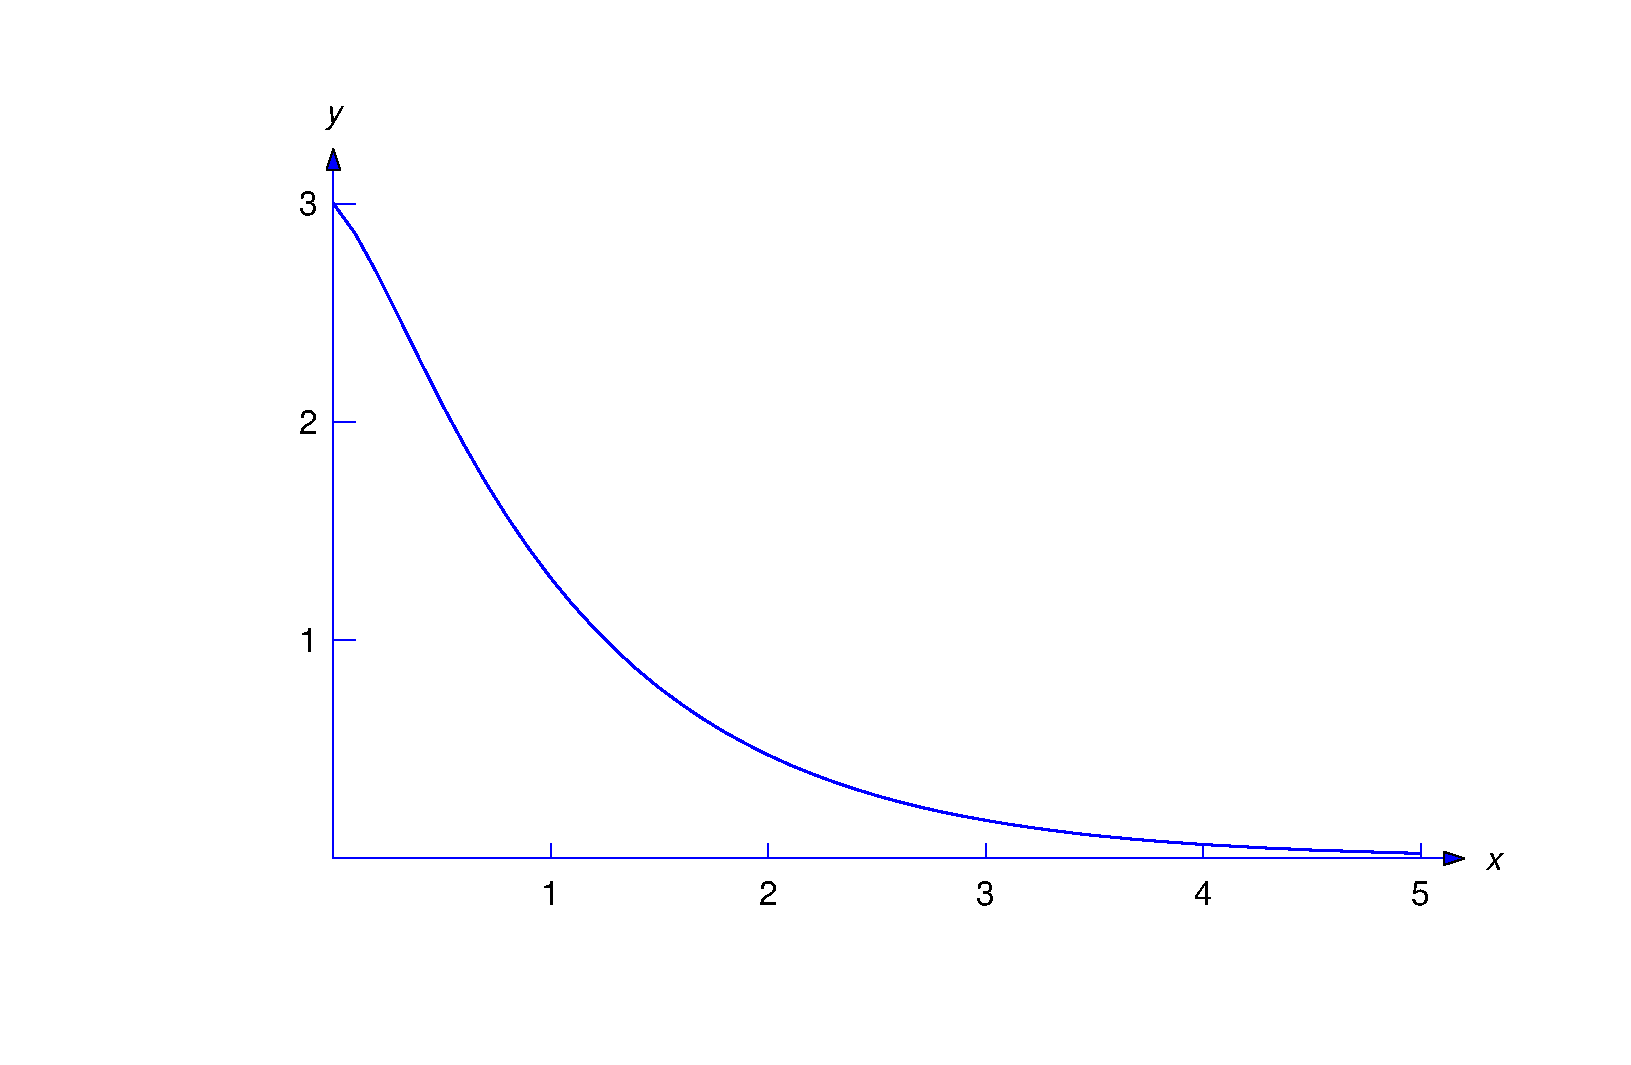
\includegraphics[bb=-78 148 689 643,width=5.67in,height=3.66in,keepaspectratio]{fig050201}
\color{blue}
  \caption{$y=\dst{{7\over2}e^{-x}-{1\over2}e^{-5x}}$ }
  \label{figure:5.2.1}
\end{figure}

If the characteristic equation has arbitrary distinct real roots
$r_1$ and $r_2$, then
$y_1=e^{r_1x}$ and $y_2=e^{r_2x}$  are  solutions of $ay''+by'+cy=0$.
Since $y_2/y_1=e^{(r_2-r_1)x}$ is nonconstant, Theorem~\ref{thmtype:5.1.6}
 implies that  $\{y_1,y_2\}$ is a fundamental
set of solutions of $ay''+by'+cy=0$.

\newpage
\boxit{Case 2: A Repeated Real Root}

\noindent
\begin{example}\label{example:5.2.2}\rm \mbox{}\newline
\begin{alist}
\item %(a)
Find the general solution of
\begin{equation} \label{eq:5.2.8}
y''+6y'+9y=0.
\end{equation}

\item %(b)
Solve the initial value problem
\begin{equation} \label{eq:5.2.9}
y''+6y'+9y=0, \quad   y(0)=3,\;  y'(0)=-1.
\end{equation}
\end{alist}
\end{example}

\solutionpart{a}   The characteristic polynomial of
 \eqref{eq:5.2.8} is
$$
p(r)=r^2+6r+9=(r+3)^2,
$$
so the characteristic equation has the repeated real root $r_1=-3$.
Therefore $y_1=e^{-3x}$ is a solution of \eqref{eq:5.2.8}. Since the
characteristic equation has no other roots, \eqref{eq:5.2.8}
has no other  solutions of the form $e^{rx}$.
 We  look for  solutions of the form
$y=uy_1=ue^{-3x}$,
where $u$ is a function that we'll now
determine.
(This should remind you of the method of variation of parameters
used in Section~2.1 to solve the nonhomogeneous
equation $y'+p(x)y=f(x)$, given a solution $y_1$ of the complementary
equation $y'+p(x)y=0$.  It's also a special case of a method called
{\color{blue}\it reduction of order\/} that we'll study in Section~5.6.
For other ways to obtain a second solution of \eqref{eq:5.2.8} that's
not a multiple of $e^{-3x}$, see
Exercises~5.1.~\hspace*{-3pt}\ref{exer:5.1.9},
5.1.~\hspace*{-3pt}\ref{exer:5.1.12}, and \ref{exer:5.2.33}.

If $y=ue^{-3x}$, then
$$
y'=u'e^{-3x}-3ue^{-3x}\mbox{\quad and \quad}
y''=u''e^{-3x}-6u'e^{-3x}+9ue^{-3x},
$$
so
\begin{eqnarray*}
y''+6y'+9y&=&e^{-3x}\left[(u''-6u'+9u)+6(u'-3u)+9u\right]\\
&=&e^{-3x}\left[u''-(6-6)u'+(9-18+9)u\right]=u''e^{-3x}.
\end{eqnarray*}
Therefore $y=ue^{-3x}$ is a solution of \eqref{eq:5.2.8} if and only if
$u''=0$, which is equivalent to $u=c_1+c_2x$, where $c_1$ and $c_2$
are constants. Therefore any function of the form
\begin{equation} \label{eq:5.2.10}
y=e^{-3x}(c_1+c_2x)
\end{equation}
is  a solution of \eqref{eq:5.2.8}.
Letting $c_1=1$ and $c_2=0$  yields the solution
 $y_1=e^{-3x}$ that we already knew. Letting $c_1=0$ and $c_2=1$
yields the second solution $y_2=xe^{-3x}$. Since
$y_2/y_1=x$
is nonconstant, \ref{thmtype:5.1.6} implies that   $\{y_1,y_2\}$ is
fundamental set of solutions of \eqref{eq:5.2.8}, and \eqref{eq:5.2.10}
is the general solution.

\solutionpart{b}  Differentiating   \eqref{eq:5.2.10} yields
\begin{equation} \label{eq:5.2.11}
y'=-3e^{-3x}(c_1+c_2x)+c_2e^{-3x}.
\end{equation}
Imposing the initial conditions $y(0)=3,\, y'(0)=-1$ in \eqref{eq:5.2.10}
and \eqref{eq:5.2.11} yields $c_1=3$ and $-3c_1+c_2=-1$, so
$c_2=8$. Therefore the solution of \eqref{eq:5.2.9} is
$$
y=e^{-3x}(3+8x).
$$
Figure~\ref{figure:5.2.2} is a graph of this solution.

\enlargethispage{2in}

\begin{figure}[H]
  \centering
  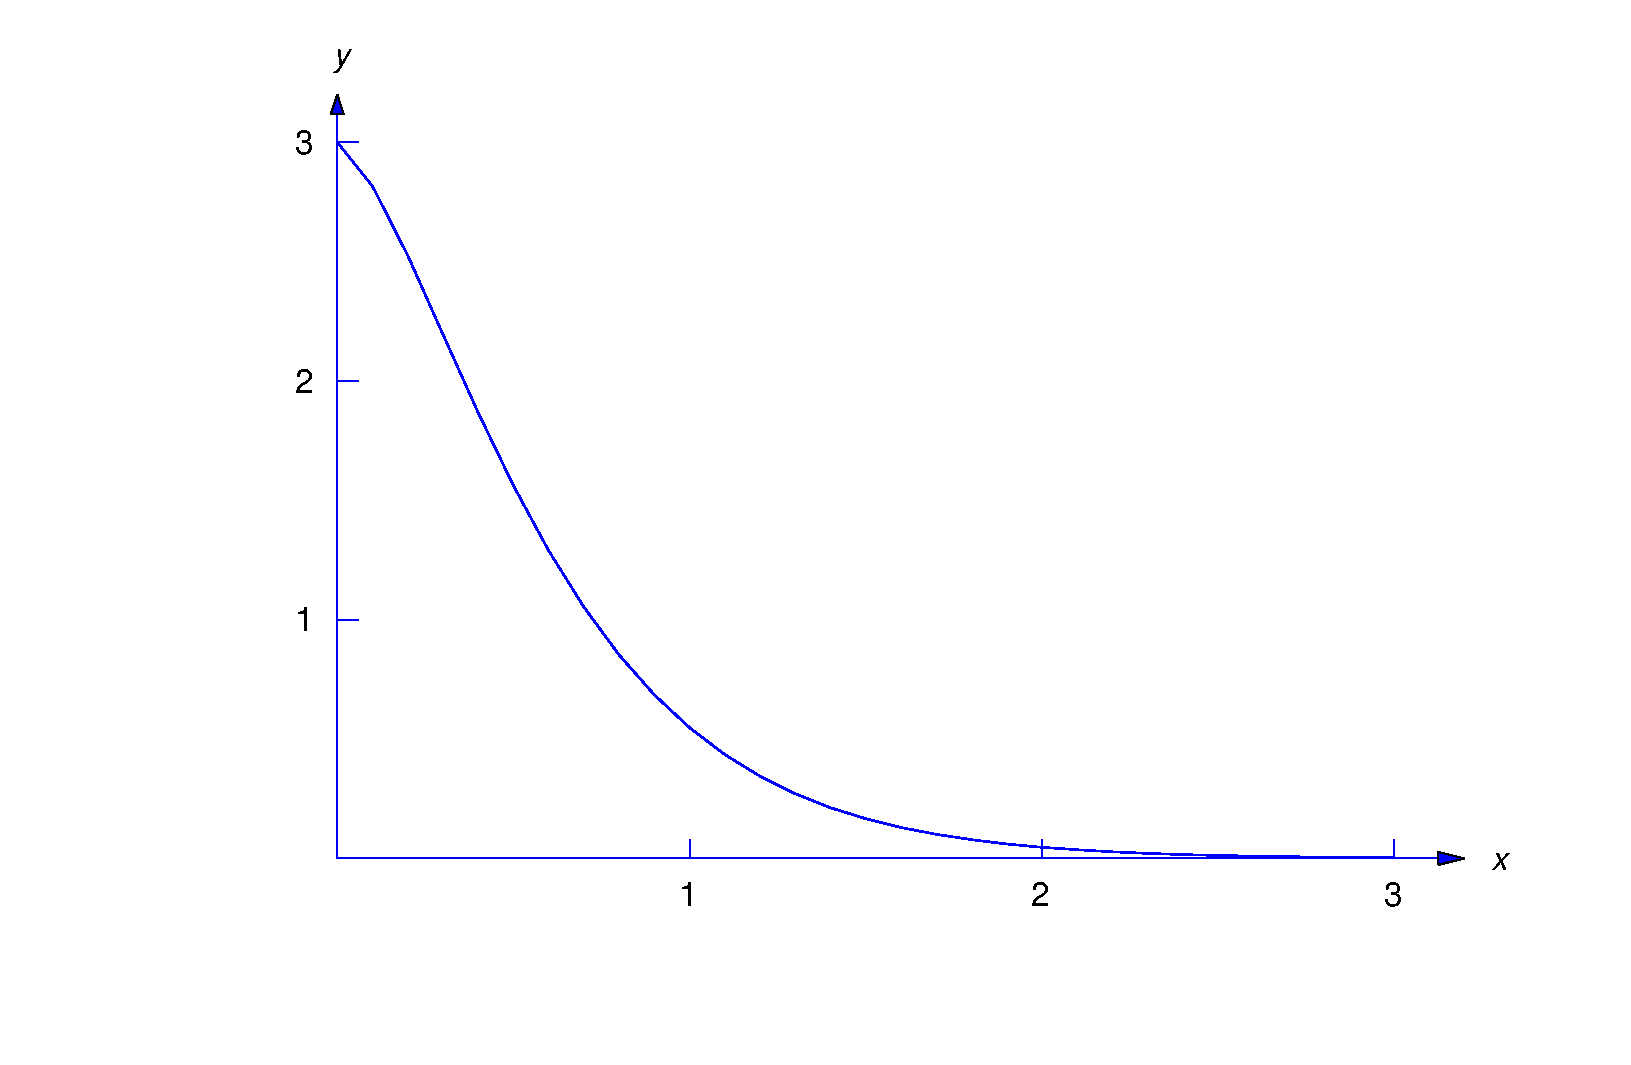
\includegraphics[bb=-78 148 689 643,width=5.67in,height=3.66in,keepaspectratio]{fig050202}
\color{blue}
\vspace*{-10pt}
  \caption{$y=e^{-3x}(3+8x)$}
  \label{figure:5.2.2}
\end{figure}

\newpage
If the characteristic equation of $ay''+by'+cy=0$
has an arbitrary repeated root $r_1$,  the
characteristic polynomial must be
$$
p(r)=a(r-r_1)^2=a(r^2-2r_1r+r_1^2).
$$
Therefore
$$
ar^2+br+c=ar^2-(2ar_1)r+ar_1^2,
$$
which implies that $b=-2ar_1$ and $c=ar_1^2$.
Therefore
 $ay''+by'+cy=0$ can be written as
$a(y''-2r_1y'+r_1^2y)=0$. Since $a\ne0$ this equation has the same
solutions as
\begin{equation} \label{eq:5.2.12}
y''-2r_1y'+r_1^2y=0.
\end{equation}

Since $p(r_1)=0$, t $y_1=e^{r_1x}$ is a solution of
$ay''+by'+cy=0$, and therefore of \eqref{eq:5.2.12}. Proceeding as in
Example~\ref{example:5.2.2}, we look for other solutions of \eqref{eq:5.2.12}
of the form $y=ue^{r_1x}$; then
$$
y'=u'e^{r_1x}+rue^{r_1x}\mbox{\quad and \quad}
y''=u''e^{r_1x}+2r_1u'e^{r_1x}+r_1^2ue^{r_1x},
$$
so
\begin{eqnarray*}
y''-2r_1y'+r_1^2y&=&e^{rx}\left[(u''+2r_1u'+r_1^2u)-
2r_1(u'+r_1u)+r_1^2u\right]\\
&=&e^{r_1x}\left[u''+(2r_1-2r_1)u'+(r_1^2-2r_1^2+r_1^2)u\right]=u''e^{r_1x}.
\end{eqnarray*}
Therefore $y=ue^{r_1x}$ is a solution of \eqref{eq:5.2.12} if and only if
$u''=0$, which is equivalent to $u=c_1+c_2x$, where $c_1$ and $c_2$
are constants. Hence, any function of the form
\begin{equation} \label{eq:5.2.13}
y=e^{r_1x}(c_1+c_2x)
\end{equation}
is  a solution of \eqref{eq:5.2.12}.
Letting $c_1=1$ and $c_2=0$ here yields the solution
 $y_1=e^{r_1x}$ that we already knew. Letting $c_1=0$ and $c_2=1$
yields the second solution $y_2=xe^{r_1x}$. Since
$y_2/y_1=x$
is nonconstant, \ref{thmtype:5.1.6} implies that   $\{y_1,y_2\}$ is
a fundamental set of solutions of \eqref{eq:5.2.12}, and \eqref{eq:5.2.13}
is the general solution.

\boxit{Case 3: Complex Conjugate Roots}

\vspace*{-20pt}
\noindent
\begin{example}\label{example:5.2.3}\rm \mbox{}\newline
\begin{alist}
\item %(a)
Find the general solution of
\begin{equation} \label{eq:5.2.14}
y''+4y'+13y=0.
\end{equation}

\item %(b)
Solve the initial value problem
\begin{equation} \label{eq:5.2.15}
y''+4y'+13y=0, \quad   y(0)=2,\;  y'(0)=-3.
\end{equation}
\end{alist}
\end{example}

\solutionpart{a}  The characteristic
polynomial of
 \eqref{eq:5.2.14} is
$$
p(r)=r^2+4r+13=r^2+4r+4+9=(r+2)^2+9.
$$
The roots of the characteristic equation are $r_1=-2+3i$ and
$r_2=-2-3i$. By analogy with Case~1, it's reasonable to expect that
$e^{(-2+3i)x}$ and $e^{(-2-3i)x}$ are solutions of \eqref{eq:5.2.14}. This
is true (see Exercise~\ref{exer:5.2.34});     however, there are
difficulties here, since you are probably not familiar with
exponential functions with complex arguments, and even if you are, it's
 inconvenient to work with them, since they are complex--valued. We'll
 take a simpler approach, which we motivate as follows: the
exponential notation suggests that
$$
e^{(-2+3i)x}=e^{-2x}e^{3ix}\mbox{\quad and \quad}
e^{(-2-3i)x}=e^{-2x}e^{-3ix},
$$
so even though we haven't defined $e^{3ix}$ and $e^{-3ix}$, it's
reasonable to expect that every linear
combination of $e^{(-2+3i)x}$ and $e^{(-2-3i)x}$ can be written as
$y=ue^{-2x}$, where $u$ depends upon $x$. To determine $u$, we note
that if $y=ue^{-2x}$ then
$$
y'=u'e^{-2x}-2ue^{-2x}\mbox{\quad and \quad}
y''=u''e^{-2x}-4u'e^{-2x}+4ue^{-2x},
$$
so
\begin{eqnarray*}
y''+4y'+13y&=&e^{-2x}\left[(u''-4u'+4u)+4(u'-2u)+13u\right]\\
&=&e^{-2x}\left[u''-(4-4)u'+(4-8+13)u\right]=e^{-2x}(u''+9u).
\end{eqnarray*}
Therefore $y=ue^{-2x}$ is a solution of \eqref{eq:5.2.14} if and only if
$$
u''+9u=0.
$$
From Example~\ref{example:5.1.2}, the  general solution of this equation is
$$
u=c_1\cos 3x +c_2\sin 3x.
$$
 Therefore any function of the form
\begin{equation} \label{eq:5.2.16}
y=e^{-2x}(c_1\cos 3x+c_2\sin 3x)
\end{equation}
is  a solution of \eqref{eq:5.2.14}.
Letting $c_1=1$ and $c_2=0$  yields the solution
 $y_1=e^{-2x}\cos3x$. Letting $c_1=0$ and $c_2=1$
yields the second solution $y_2=e^{-2x}\sin3x$. Since
$y_2/y_1=\tan3x$
is nonconstant, \ref{thmtype:5.1.6} implies that   $\{y_1,y_2\}$ is
a fundamental set of solutions of \eqref{eq:5.2.14}, and \eqref{eq:5.2.16}
is the general solution.

\solutionpart{b}   Imposing the condition $y(0)=2$
in   \eqref{eq:5.2.16} shows that $c_1=2$.  Differentiating
\eqref{eq:5.2.16} yields
$$
y'=-2e^{-2x}(c_1\cos 3x+c_2\sin 3x) +3e^{-2x}(-c_1\sin 3x +c_2\cos 3x),
$$
and imposing the initial condition $y'(0)=-3$ here yields
$-3=-2c_1+3c_2=-4+3c_2$,
 so $c_2=1/3$. Therefore the solution of
\eqref{eq:5.2.15} is
$$
y=e^{-2x}(2\cos 3x+ {1\over3}\sin 3x).
$$
Figure~\ref{figure:5.2.3}  is a graph of this function. \bbox

      \begin{figure}[tbp]
  \centering
\color{blue}
  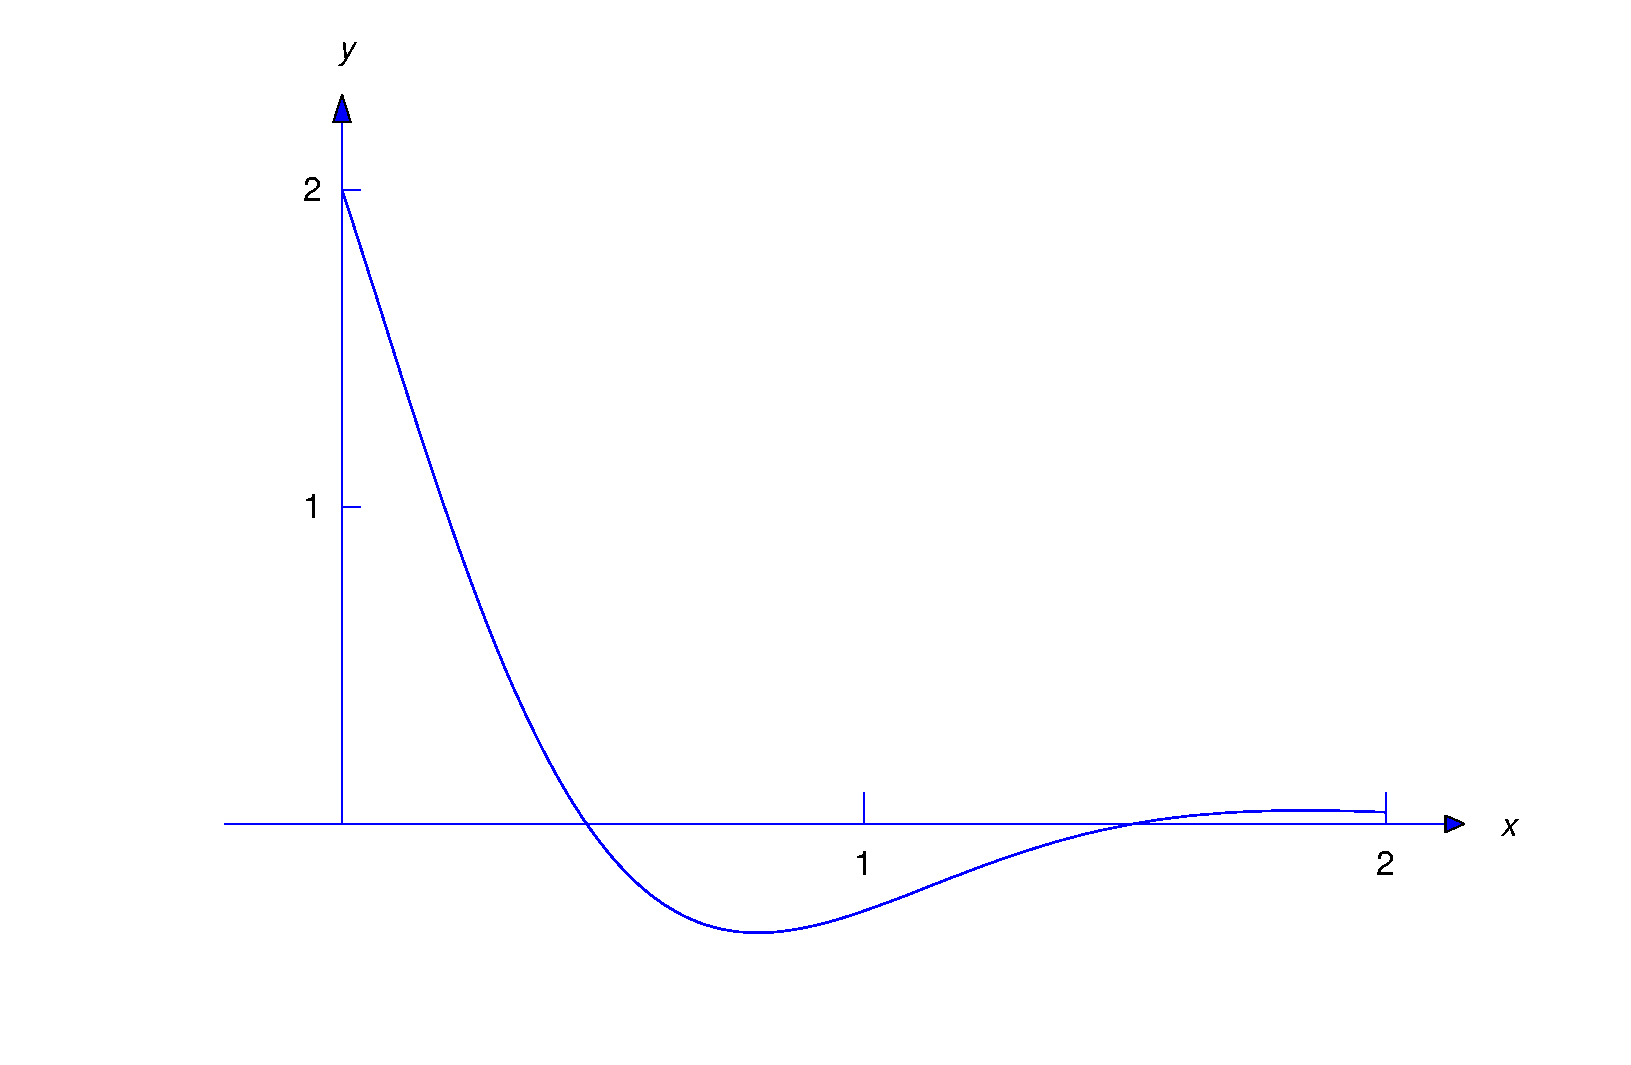
\includegraphics[bb=-78 148 689 643,width=5.67in,height=3.66in,keepaspectratio]{fig050203}
  \caption{$\dst{y=e^{-2x}(2\cos 3x+ {1\over3}\sin 3x)}$}
  \label{figure:5.2.3}
\end{figure}

Now suppose   the characteristic equation of $ay''+by'+cy=0$ has
arbitrary complex roots;   thus, $b^2-4ac<0$ and, from \eqref{eq:5.2.3},
the
roots are
$$
r_1 = {-b+i\sqrt{4ac-b^2}\over 2a},\quad r_2 =
{-b-i\sqrt{4ac-b^2}\over 2a},
$$
which we rewrite as
\begin{equation} \label{eq:5.2.17}
r_1=\lambda+i \omega,\quad r_2 = \lambda - i \omega,
\end{equation}
 with
$$
\lambda = -{b\over 2a},\quad \omega = {\sqrt{4ac-b^2}\over 2a}.
$$
Don't memorize these formulas. Just remember that $r_1$
and $r_2$ are of the form \eqref{eq:5.2.17},
where  $\lambda$ is an arbitrary real number and $\omega$
is   positive;
 $\lambda$ and $\omega$ are  the {\color{blue}\it real\/}
and {\color{blue}\it imaginary parts\/}, respectively, of $r_1$.
Similarly, $\lambda$ and $-\omega$ are the real and imaginary parts of
$r_2$. We say that $r_1$ and $r_2$ are {\color{blue}\it complex conjugates\/},
which means that they have the same real part and their imaginary
parts have the same absolute values, but opposite signs.

As in Example~\ref{example:5.2.3}, it's reasonable to
to expect that the solutions of $ay''+by'+cy=0$  are linear
combinations of
$e^{(\lambda+i\omega)x}$ and $e^{(\lambda-i\omega)x}$.
Again,  the exponential notation suggests that
$$
e^{(\lambda+i\omega)x}=e^{\lambda x}e^{i\omega x}\mbox{\quad and
\quad} e^{(\lambda-i\omega)x}=e^{\lambda x}e^{-i\omega x},
$$
so even though we haven't defined $e^{i\omega x}$ and
$e^{-i\omega x}$, it's reasonable to expect that every linear
combination of $e^{(\lambda+i\omega)x}$ and $e^{(\lambda-i\omega)x}$
can  be written as
$y=ue^{\lambda x}$, where $u$ depends upon $x$.
To determine $u$ we first observe that since $r_1=\lambda+i\omega$
and $r_2=\lambda-i\omega$ are the roots of the characteristic
equation,  $p$ must be of  the form
$$
\begin{array}{ccl}
p(r)&=&a(r-r_1)(r-r_2)\\
&=&a(r-\lambda-i\omega)(r-\lambda+i\omega)\\
&=& a \left[(r-\lambda)^2+\omega^2\right]\\
&=&a(r^2-2\lambda r +\lambda^2+\omega^2).
\end{array}
$$
Therefore $ay''+by'+cy=0$ can be written as
$$
a\left[y''-2\lambda y'+(\lambda^2+\omega^2)y\right]=0.
$$
 Since $a\ne0$
this equation has the same solutions as
\begin{equation} \label{eq:5.2.18}
y''-2\lambda y'+(\lambda^2+\omega^2)y=0.
\end{equation}
 To determine $u$ we note
that if $y=ue^{\lambda x}$ then
$$
y'=u'e^{\lambda x}+\lambda ue^{\lambda x}\mbox{\quad and \quad}
y''=u''e^{\lambda x}+2\lambda u'e^{\lambda x}+\lambda^2ue^{\lambda x}.
$$
Substituting these expressions  into
\eqref{eq:5.2.18} and dropping the common factor $e^{\lambda x}$ yields
$$
(u''+2\lambda u'+\lambda^2 u)-2\lambda(u'+\lambda u)
+(\lambda^2+\omega^2)u=0,
$$
which simplifies to
$$
u''+\omega^2 u=0.
$$
From Example~\ref{example:5.1.2}, the  general solution of this
equation is
$$
u=c_1\cos\omega x +c_2\sin\omega x.
$$
 Therefore any function of the form
\begin{equation} \label{eq:5.2.19}
y=e^{\lambda x}(c_1\cos\omega x+c_2\sin\omega x)
\end{equation}
is  a solution of \eqref{eq:5.2.18}.
Letting $c_1=1$ and $c_2=0$ here yields the solution
 $y_1=e^{\lambda x}\cos\omega x$. Letting $c_1=0$ and $c_2=1$
yields a second solution $y_2=e^{\lambda x}\sin\omega x$. Since
$y_2/y_1=\tan\omega x$
is nonconstant, so  Theorem~\ref{thmtype:5.1.6} implies that
$\{y_1,y_2\}$ is
a fundamental set of solutions of \eqref{eq:5.2.18}, and \eqref{eq:5.2.19}
is the general solution.

\boxit{Summary}

\noindent
The next theorem summarizes the results of this section.

\begin{theorem}\color{blue} \label{thmtype:5.2.1}
Let $p(r)=ar^2+br+c$ be the characteristic polynomial of
\begin{equation} \label{eq:5.2.20}
ay''+by'+cy=0.
\end{equation}
Then$:$
\begin{alist}
\item % (a)
If $p(r)=0$  has distinct real roots $r_1$ and $r_2,$ then the general
solution of $\eqref{eq:5.2.20}$ is
$$
y=c_1e^{r_1x}+c_2e^{r_2x}.
$$
\item % (b)
If $p(r)=0$  has a repeated root  $r_1,$ then
the general solution of $\eqref{eq:5.2.20}$ is
$$
y=e^{r_1x}(c_1+c_2x).
$$
\item % (c)
If $p(r)=0$  has complex conjugate roots $r_1=\lambda+i\omega$ and
$r_2=\lambda-i\omega$ $($where $\omega>0),$ then the general solution
of $\eqref{eq:5.2.20}$ is
$$
y=e^{\lambda x}(c_1\cos\omega x+c_2\sin\omega x).
$$
\end{alist}
\end{theorem}

\exercises
 In Exercises \ref{exer:5.2.1}--\ref{exer:5.2.12} find the general solution.

\begin{exerciselist}
\begin{tabular}[t]{@{}p{168pt}@{}p{168pt}}
 \item\label{exer:5.2.1} $y''+5y'-6y=0$
& \vspace*{10pt} \item\label{exer:5.2.2} $y''-4y'+5y=0$
\end{tabular}

\begin{tabular}[t]{@{}p{168pt}@{}p{168pt}}
 \item\label{exer:5.2.3} $y''+8y'+7y=0$
&  \item\label{exer:5.2.4} $y''-4y'+4y=0$
\end{tabular}

\begin{tabular}[t]{@{}p{168pt}@{}p{168pt}}
 \item\label{exer:5.2.5} $y''+2y'+10y=0$
&  \item\label{exer:5.2.6} $y''+6y'+10y=0$
\end{tabular}

\begin{tabular}[t]{@{}p{168pt}@{}p{168pt}}
 \item\label{exer:5.2.7} $y''-8y'+16y=0$
&  \item\label{exer:5.2.8} $y''+y'=0$
\end{tabular}

\begin{tabular}[t]{@{}p{168pt}@{}p{168pt}}
 \item\label{exer:5.2.9} $y''-2y'+3y=0$
& \item\label{exer:5.2.10} $y''+6y'+13y=0 $
\end{tabular}

\begin{tabular}[t]{@{}p{168pt}@{}p{168pt}}
  \item\label{exer:5.2.11} $4y''+4y'+10y=0$&
 \item\label{exer:5.2.12} $10y''-3y'-y=0$
\end{tabular}

\exercisetext{In Exercises \ref{exer:5.2.13}--\ref{exer:5.2.17} solve
the initial value problem.}

\item\label{exer:5.2.13}
$y''+14y'+50y=0, \quad  y(0)=2,\quad y'(0)=-17$

\item\label{exer:5.2.14}
$6y''-y'-y=0, \quad  y(0)=10,\quad y'(0)=0$

\item\label{exer:5.2.15}
$6y''+y'-y=0, \quad  y(0)=-1,\quad y'(0)=3$

\item\label{exer:5.2.16}
$4y''-4y'-3y=0, \quad  y(0)=\dst{13\over 12},\quad y'(0)=\dst{23
\over 24}$

\item\label{exer:5.2.17}
$4y''-12y'+9y=0, \quad  y(0)=3,\quad y'(0)=\dst{5\over 2}$

\exercisetext{In Exercises \ref{exer:5.2.18}--\ref{exer:5.2.21} solve
the initial value problem and graph the solution.}

\item\label{exer:5.2.18} \CGex
$y''+7y'+12y=0, \quad  y(0)=-1,\quad y'(0)=0$

\item\label{exer:5.2.19} \CGex
$y''-6y'+9y=0, \quad  y(0)=0,\quad y'(0)=2$

\item\label{exer:5.2.20} \CGex
$36y''-12y'+y=0, \quad  y(0)=3,\quad y'(0)=\dst{5\over2}$

\item\label{exer:5.2.21} \CGex
$y''+4y'+10y=0, \quad  y(0)=3,\quad y'(0)=-2$

\item\label{exer:5.2.22}
\begin{alist}
\item % (a)
Suppose $y$  is a solution of the constant coefficient homogeneous
equation
$$
ay''+by'+cy=0.
\eqno{\rm (A)}
$$
Let $z(x)=y(x-x_0)$, where $x_0$ is an arbitrary real number.
Show that
$$
az''+bz'+cz=0.
$$
\item % (b)
Let $z_1(x)=y_1(x-x_0)$ and $z_2(x)=y_2(x-x_0)$, where $\{y_1,y_2\}$
is a fundamental set of solutions of (A). Show that
$\{z_1,z_2\}$ is also a fundamental set of solutions of
(A).

\item % (c)
The statement of
 Theorem~\ref{thmtype:5.2.1}  is convenient for solving an
initial value problem
$$
ay''+by'+cy=0, \quad  y(0)=k_0,\quad y'(0)=k_1,
$$
where the initial conditions are imposed at $x_0=0$.
However, if the  initial value problem is
$$
ay''+by'+cy=0, \quad  y(x_0)=k_0,\quad y'(x_0)=k_1,
\eqno{\rm (B)}
$$
where $x_0\ne0$, then  determining  the constants in
$$
y=c_1e^{r_1x}+c_2e^{r_2x}, \quad  y=e^{r_1x}(c_1+c_2x),\mbox{ or }
y=e^{\lambda x}(c_1\cos\omega x+c_2\sin\omega x)
$$
(whichever is applicable) is more complicated. Use \part{b} to restate
Theorem~\ref{thmtype:5.2.1} in a form more convenient for solving
(B).
\end{alist}

\exercisetext{In Exercises \ref{exer:5.2.23}--\ref{exer:5.2.28} use a method
suggested by Exercise~\ref{exer:5.2.22} to solve the initial value
problem.}

\item\label{exer:5.2.23}
$y''+3y'+2y=0, \quad  y(1)=-1,\quad y'(1)=4$
\newpage

\item\label{exer:5.2.24}
$y''-6y'-7y=0, \quad  y(2)=-\dst{1\over3},\quad y'(2)=-5$

\item\label{exer:5.2.25}
$y''-14y'+49y=0, \quad  y(1)=2,\quad y'(1)=11$

\item\label{exer:5.2.26}
$9y''+6y'+y=0, \quad  y(2)=2,\quad y'(2)=-\dst{14\over3}$

\item\label{exer:5.2.27}
$9y''+4y=0, \quad  y(\pi/4)=2,\quad y'(\pi/4)=-2$

\item\label{exer:5.2.28}
$y''+3y=0, \quad  y(\pi/3)=2,\quad y'(\pi/3)=-1$

\item\label{exer:5.2.29}
Prove: If the characteristic equation of
$$
ay''+by'+cy=0
\eqno{\rm (A)}
$$
has a repeated negative root or two roots with negative real parts, then
every solution of  (A) approaches zero as $x\to\infty$.

\item\label{exer:5.2.30}
Suppose  the characteristic polynomial of $ay''+by'+cy=0$
 has distinct real roots $r_1$ and $r_2$. Use a method suggested
by Exercise~\ref{exer:5.2.22}  to find a formula for the solution
of
$$
ay''+by'+cy=0, \quad  y(x_0)=k_0,\quad y'(x_0)=k_1.
$$

\item\label{exer:5.2.31}
Suppose the characteristic polynomial of $ay''+by'+cy=0$ has a
repeated real root $r_1$. Use a method suggested by
Exercise~\ref{exer:5.2.22} to find a formula for the solution of
$$
ay''+by'+cy=0, \quad  y(x_0)=k_0,\quad y'(x_0)=k_1.
$$

\item\label{exer:5.2.32}
Suppose the characteristic polynomial of $ay''+by'+cy=0$ has
complex conjugate roots $\lambda\pm i\omega$. Use a method suggested
by Exercise~\ref{exer:5.2.22} to find a formula for the solution of
$$
ay''+by'+cy=0, \quad  y(x_0)=k_0,\quad y'(x_0)=k_1.
$$

\item\label{exer:5.2.33}
Suppose the characteristic equation of
$$
ay''+by'+cy=0
\eqno{\rm (A)}
$$
has a repeated real root $r_1$. Temporarily, think of $e^{rx}$
as a function of two real variables $x$ and $r$.
\begin{alist}
\item % (a)
Show that
$$
a{\partial^2\over\partial^2 x}(e^{rx})+b{\partial \over\partial
x}(e^{rx}) +ce^{rx}=a(r-r_1)^2e^{rx}.
\eqno{\rm (B)}
$$
\item % (b)
Differentiate (B) with respect to $r$  to obtain
$$
a{\partial\over\partial r}\left({\partial^2\over\partial^2
x}(e^{rx})\right)+b{\partial\over\partial r}\left({\partial
\over\partial x}(e^{rx})\right)
+c(xe^{rx})=[2+(r-r_1)x]a(r-r_1)e^{rx}.
\eqno{\rm (C)}
$$
\item % (c)
Reverse the orders of the partial differentiations in the first two
terms on the left side of
(C) to obtain
$$
a{\partial^2\over\partial x^2}(xe^{rx})+b{\partial\over\partial
x}(xe^{rx})+c(xe^{rx})=[2+(r-r_1)x]a(r-r_1)e^{rx}.
\eqno{\rm (D)}
$$
\item % (d)
Set $r=r_1$ in (B) and (D)
to see that $y_1=e^{r_1x}$ and $y_2=xe^{r_1x}$ are solutions
of (A)
\end{alist}

\item\label{exer:5.2.34}
In calculus you learned that $e^u$, $\cos u$, and $\sin u$
can be represented by the infinite series
$$
e^u=\sum_{n=0}^\infty {u^n\over n!}
=1+{u\over 1!}+{u^2\over 2!}+{u^3\over 3!}+\cdots+{u^n\over
n!}+\cdots
\eqno{\rm (A)}
$$
$$
\cos u=\sum_{n=0}^\infty (-1)^n{u^{2n}\over(2n)!}
=1-{u^2\over2!}+{u^4\over4!}+\cdots+(-1)^n{u^{2n}\over(2n)!}
+\cdots,
\eqno{\rm (B)}
$$
and
$$
\sin u=\sum_{n=0}^\infty (-1)^n{u^{2n+1}\over(2n+1)!}
=u-{u^3\over3!}+{u^5\over5!}+\cdots+(-1)^n
{u^{2n+1}\over(2n+1)!}
+\cdots
\eqno{\rm (C)}
$$
for all real values of $u$.
Even though you have previously considered (A)
only for real values of $u$, we can set $u=i\theta$, where $\theta$ is
real, to obtain
$$
e^{i\theta}=\sum_{n=0}^\infty {(i\theta)^n\over n!}.
\eqno{\rm (D)}
$$
Given the proper background in the theory of infinite series with
complex terms, it can be shown that the series in
(D) converges for all real $\theta$.
\begin{alist}
\item % (a)
Recalling that $i^2=-1,$
write enough  terms of the sequence $\{i^n\}$ to convince yourself
that the sequence is repetitive:
$$
1,i,-1,-i,1,i,-1,-i,1,i,-1,-i,1,i,-1,-i,\cdots.
$$
Use this to group the terms in (D) as
\begin{eqnarray*}
e^{i\theta}&=&\left(1-{\theta^2\over2}+{\theta^4\over4}+\cdots\right)
+i\left(\theta-{\theta^3\over3!}+{\theta^5\over5!}+\cdots\right)\\[2\jot]
&=&\sum_{n=0}^\infty (-1)^n{\theta^{2n}\over(2n)!}
+i\sum_{n=0}^\infty (-1)^n{\theta^{2n+1}\over(2n+1)!}.
\end{eqnarray*}
By comparing this result with (B) and
(C), conclude that
$$
e^{i\theta}=\cos\theta+i\sin\theta.
\eqno{\rm (E)}
$$
This is
\href{http://www-history.mcs.st-and.ac.uk/Mathematicians/Euler.html}
{\color{blue}\it Euler's identity\/}.
\item % (b)
Starting from
$$
e^{i\theta_1}e^{i\theta_2}=(\cos\theta_1+i\sin\theta_1)
(\cos\theta_2+i\sin\theta_2),
$$
collect the real part (the terms not multiplied by $i$)
and the imaginary part (the terms  multiplied by $i$) on the
right, and use the trigonometric identities
\begin{eqnarray*}
\cos(\theta_1+\theta_2)&=&\cos\theta_1\cos\theta_2-\sin\theta_1\sin\theta_2\\
\sin(\theta_1+\theta_2)&=&\sin\theta_1\cos\theta_2+\cos\theta_1\sin\theta_2
\end{eqnarray*}
to verify that
$$
e^{i(\theta_1+\theta_2)}=e^{i\theta_1}e^{i\theta_2},
$$
as you would expect from the use of the exponential notation
$e^{i\theta}$.
\item % (c)
If  $\alpha$ and $\beta$ are real numbers,
define
$$
e^{\alpha+i\beta}=e^\alpha e^{i\beta}=e^\alpha(\cos\beta+i\sin\beta).
\eqno{\rm (F)}
$$
Show that if $z_1=\alpha_1+i\beta_1$ and $z_2=\alpha_2+i\beta_2$ then
$$
e^{z_1+z_2}=e^{z_1}e^{z_2}.
$$
\item % (d)
Let $a$, $b$, and $c$ be real numbers, with $a\ne0$. Let $z=u+iv$
where $u$ and $v$ are real-valued functions of $x$. Then we say that
$z$ is a solution of
$$
ay''+by'+cy=0
\eqno{\rm (G)}
$$
if $u$ and $v$ are both solutions of (G).
Use   Theorem~\ref{thmtype:5.2.1}\part{c} to verify that if the
characteristic equation of (G) has complex conjugate roots
$\lambda\pm i\omega$ then
$z_1=e^{(\lambda+i\omega)x}$ and $z_2=e^{(\lambda-i\omega)x}$
are both solutions of (G).
\end{alist}
\end{exerciselist}


\section{Nonhomogeneous Linear Equations}

\noindent
We'll now consider the nonhomogeneous linear second order equation
\begin{equation}
  \label{eq:5.3.1}y''+p(x)y'+q(x)y=f(x),
\end{equation}
where the forcing function $f$ isn't identically zero. The next theorem, an extension of
Theorem~\ref{thmtype:5.1.1}, gives sufficient conditions for existence and uniqueness of solutions
of initial value problems for \eqref{eq:5.3.1}. We omit the proof, which is beyond the scope of this
book.

\begin{theorem}
  \color{blue}
  \label{thmtype:5.3.1} Suppose $p$, $q$, and $f$ are continuous on an open interval $(a,b)$, let
  $x_{0}$ be any point in $(a,b)$, and let $k_{0}$ and $k_{1}$ be arbitrary real numbers. Then the
  initial value problem
  \[
    y''+p(x)y'+q(x)y=f(x),\quad y(x_{0})=k_{0},\quad y'(x_{0})=k_{1}
  \]
  has a unique solution on $(a,b)$.
\end{theorem}

To find the general solution of \eqref{eq:5.3.1} on an interval $(a,b)$ where $p$, $q$, and $f$ are
continuous, it's necessary to find the general solution of the associated homogeneous equation
\begin{equation}
  \label{eq:5.3.2}y''+p(x)y'+q(x)y=0
\end{equation}
on $(a,b)$. We call \eqref{eq:5.3.2} the {\color{blue}\it complementary equation\/} for
\eqref{eq:5.3.1}.

The next theorem shows how to find the general solution of \eqref{eq:5.3.1} if we know one solution
$y_{p}$ of \eqref{eq:5.3.1} and a fundamental set of solutions of \eqref{eq:5.3.2}. We call $y_{p}$
a {\color{blue}\it particular solution\/} of \eqref{eq:5.3.1}; it can be any solution that we can
find, one way or another.

\begin{theorem}
  \color{blue}
  \label{thmtype:5.3.2} Suppose $p$, $q$, and $f$ are continuous on $(a,b)$. Let $y_{p}$ be a
  particular solution of
  \begin{equation}
    \label{eq:5.3.3}y''+p(x)y'+q(x)y=f(x)
  \end{equation}
  on $(a,b)$, and let $\{y_{1},y_{2}\}$ be a fundamental set of solutions of the complementary
  equation
  \begin{equation}
    \label{eq:5.3.4}y''+p(x)y'+q(x)y=0
  \end{equation}
  on $(a,b)$. Then $y$ is a solution of \eqref{eq:5.3.3} on $(a,b)$ if and only if
  \begin{equation}
    \label{eq:5.3.5}y=y_{p}+c_{1}y_{1}+c_{2}y_{2},
  \end{equation}
  where $c_{1}$ and $c_{2}$ are constants.
\end{theorem}

\proof We first show that $y$ in \eqref{eq:5.3.5} is a solution of \eqref{eq:5.3.3} for any choice
of the constants $c_{1}$ and $c_{2}$. Differentiating \eqref{eq:5.3.5} twice yields
\[
  y'=y_{p}'+c_{1}y_{1}'+c_{2}y_{2}'\mbox{\quad and \quad}y''=y_{p}''+c_{1}y_{1}''+c_{2}y_{2}'',
\]
so
\begin{eqnarray*}
  y''+p(x)y'+q(x)y & = & (y_{p}''+c_{1}y_{1}''+c_{2}y_{2}'')+p(x)(y_{p}'+c_{1}y_{1}'+c_{2}y_{2}') \\
                   &   & \;+q(x)(y_{p}+c_{1}y_{1}+c_{2}y_{2})                                     \\
                   & = & (y_{p}''+p(x)y_{p}'+q(x)y_{p})+c_{1}(y_{1}''+p(x)y_{1}'+q(x)y_{1})       \\
                   &   & \;+c_{2}(y_{2}''+p(x)y_{2}'+q(x)y_{2})                                   \\
                   & = & f+c_{1}\cdot0+c_{2}\cdot0=f,
\end{eqnarray*}
since $y_{p}$ satisfies \eqref{eq:5.3.3} and $y_{1}$ and $y_{2}$ satisfy \eqref{eq:5.3.4}.

Now we'll show that every solution of \eqref{eq:5.3.3} has the form \eqref{eq:5.3.5} for some choice
of the constants $c_{1}$ and $c_{2}$. Suppose $y$ is a solution of \eqref{eq:5.3.3}. We'll show that
$y-y_{p}$ is a solution of \eqref{eq:5.3.4}, and therefore of the form
$y-y_{p}=c_{1}y_{1}+c_{2}y_{2}$, which implies \eqref{eq:5.3.5}. To see this, we compute
\begin{eqnarray*}
  (y-y_{p})''+p(x)(y-y_{p})'+q(x)(y-y_{p}) & = & (y''-y_{p}'')+p(x)(y'-y_{p}')   \\
                                           &   & +q(x)(y-y_{p})                  \\
                                           & = & (y''+p(x)y'+q(x)y)              \\
                                           &   & -(y_{p}''+p(x)y_{p}'+q(x)y_{p}) \\
                                           & = & f(x)-f(x)=0,
\end{eqnarray*}
since $y$ and $y_{p}$ both satisfy \eqref{eq:5.3.3}. \bbox

We say that \eqref{eq:5.3.5} is the {\color{blue}\it general solution of \eqref{eq:5.3.3} on
$(a,b)$.\/}

If $P_{0}$, $P_{1}$, and $F$ are continuous and $P_{0}$ has no zeros on $(a,b)$, then
Theorem~\ref{thmtype:5.3.2} implies that the general solution of
\begin{equation}
  \label{eq:5.3.6}P_{0}(x)y''+P_{1}(x)y'+P_{2}(x)y=F(x)
\end{equation}
on $(a,b)$ is $y=y_{p}+c_{1}y_{1}+c_{2}y_{2}$, where $y_{p}$ is a particular solution of
\eqref{eq:5.3.6} on $(a,b)$ and $\{y_{1},y_{2}\}$ is a fundamental set of solutions of
\[
  P_{0}(x)y''+P_{1}(x)y'+P_{2}(x)y=0
\]
on $(a,b)$. To see this, we rewrite \eqref{eq:5.3.6} as
\[
  y''+\frac{P_{1}(x)}{P_{0}(x)}y'+\frac{P_{2}(x)}{P_{0}(x)}y=\frac{F(x)}{P_{0}(x)}
\]
and apply Theorem~\ref{thmtype:5.3.2} with $p=P_{1}/P_{0}$, $q=P_{2}/P_{0}$, and $f=F/P_{0}$.

To avoid awkward wording in examples and exercises, we won't specify the interval $(a,b)$ when we
ask for the general solution of a specific linear second order equation, or for a fundamental set of
solutions of a homogeneous linear second order equation. Let's agree that this always means that we
want the general solution (or a fundamental set of solutions, as the case may be) on every open
interval on which $p$, $q$, and $f$ are continuous if the equation is of the form \eqref{eq:5.3.3},
or on which $P_{0}$, $P_{1}$, $P_{2}$, and $F$ are continuous and $P_{0}$ has no zeros, if the
equation is of the form \eqref{eq:5.3.6}. We leave it to you to identify these intervals in specific
examples and exercises.

For completeness, we point out that if $P_{0}$, $P_{1}$, $P_{2}$, and $F$ are all continuous on an
open interval $(a,b)$, but $P_{0}$ {\color{blue}\it does\/} have a zero in $(a,b)$, then
\eqref{eq:5.3.6} may fail to have a general solution on $(a,b)$ in the sense just defined.
Exercises~\ref{exer:5.1.42}--\ref{exer:5.1.44} illustrate this point for a homogeneous equation.

In this section we to limit ourselves to applications of Theorem~\ref{thmtype:5.3.2} where we can
guess at the form of the particular solution.

\begin{example}
  \label{example:5.3.1} \rm \mbox{}
  \newline
  \begin{alist}
    \item % (a)
    Find the general solution of
    \begin{equation}
      \label{eq:5.3.7}y''+y=1.
    \end{equation}

    \item % (b)
    Solve the initial value problem
    \begin{equation}
      \label{eq:5.3.8}y''+y=1,\quad y(0)=2,\quad y'(0)=7.
    \end{equation}
  \end{alist}
\end{example}

\solutionpart{a} We can apply Theorem~\ref{thmtype:5.3.2} with $(a,b)=(-\infty,\infty)$, since the
functions $p\equiv0$, $q\equiv1$, and $f\equiv1$ in \eqref{eq:5.3.7} are continuous on
$(-\infty,\infty)$. By inspection we see that $y_{p}\equiv1$ is a particular solution of
\eqref{eq:5.3.7}. Since $y_{1}=\cos x$ and $y_{2}=\sin x$ form a fundamental set of solutions of the
complementary equation $y''+y=0$, the general solution of \eqref{eq:5.3.7} is
\begin{equation}
  \label{eq:5.3.9}y=1+c_{1}\cos x+c_{2}\sin x.
\end{equation}

\solutionpart{b} Imposing the initial condition $y(0)=2$ in \eqref{eq:5.3.9} yields $2=1+c_{1}$, so
$c_{1}=1$. Differentiating \eqref{eq:5.3.9} yields
\[
  y'=-c_{1}\sin x+c_{2}\cos x.
\]
Imposing the initial condition $y'(0)=7$ here yields $c_{2}=7$, so the solution of \eqref{eq:5.3.8}
is
\[
  y=1+\cos x+7\sin x.
\]
Figure~\ref{figure:5.3.1} is a graph of this function.

\begin{figure}[tbp]
  \centering
  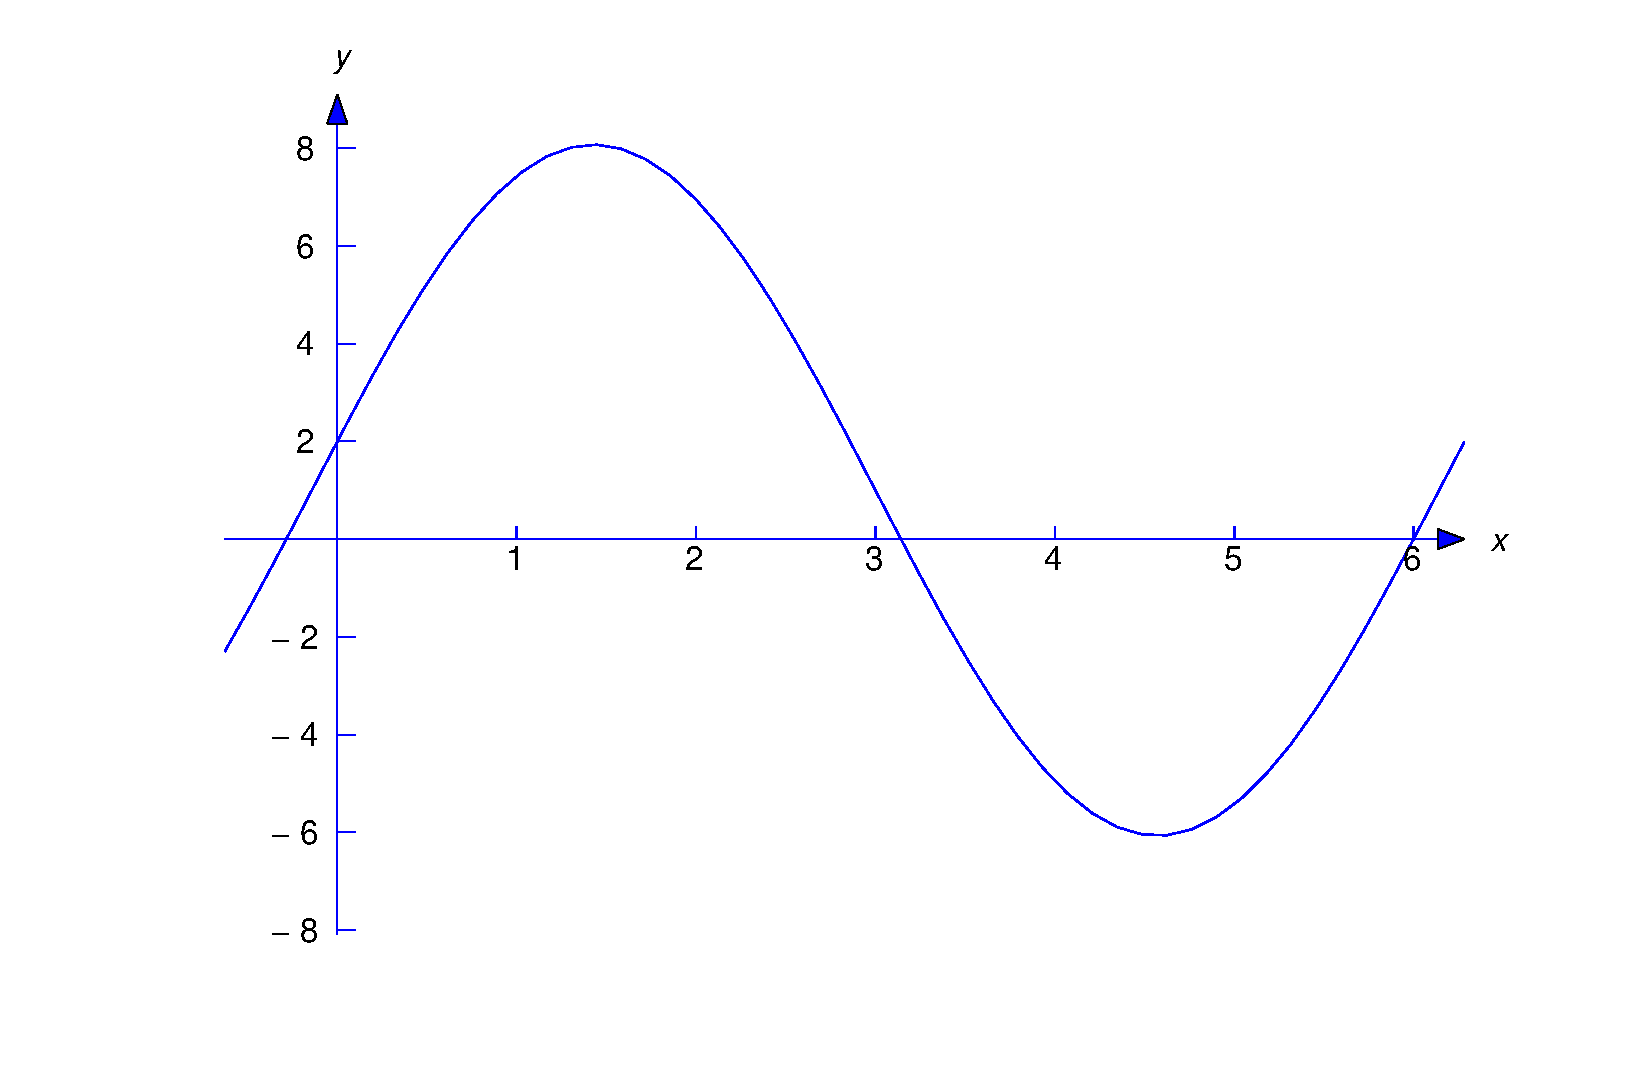
\includegraphics[bb=-78 148 689 643, width=5.67in, height=3.66in, keepaspectratio]{fig050301}
  \color{blue}
  \caption{$y=1+\cos x+7\sin x$}
  \label{figure:5.3.1}
\end{figure}

\begin{example}
  \label{example:5.3.2} \rm \mbox{}
  \newline %\examplepoly
  \begin{alist}
    \item % (a)
    Find the general solution of
    \begin{equation}
      \label{eq:5.3.10}y''-2y'+y=-3-x+x^{2}.
    \end{equation}

    \item % (b)
    Solve the initial value problem
    \begin{equation}
      \label{eq:5.3.11}y''-2y'+y=-3-x+x^{2},\quad y(0)=-2,\quad y'(0)=1.
    \end{equation}
  \end{alist}
\end{example}

\solutionpart{a} The characteristic polynomial of the complementary equation
\[
  y''-2y'+y=0
\]
is $r^{2}-2r+1=(r-1)^{2}$, so $y_{1}=e^{x}$ and $y_{2}=xe^{x}$ form a fundamental set of solutions
of the complementary equation. To guess a form for a particular solution of \eqref{eq:5.3.10}, we
note that substituting a second degree polynomial $y_{p}=A+Bx+Cx^{2}$ into the left side of
\eqref{eq:5.3.10} will produce another second degree polynomial with coefficients that depend upon
$A$, $B$, and $C$. The trick is to choose $A$, $B$, and $C$ so the polynomials on the two sides of
\eqref{eq:5.3.10} have the same coefficients; thus, if
\[
  y_{p}=A+Bx+Cx^{2}\mbox{\quad then \quad}y_{p}'=B+2Cx\mbox{\quad and \quad}y_{p}''=2C,
\]
so
\begin{eqnarray*}
  y_{p}''-2y_{p}'+y_{p} & = & 2C-2(B+2Cx)+(A+Bx+Cx^{2}) \\
                        & = & (2C-2B+A)+(-4C+B)x+Cx^{2}=-3-x+x^{2}.
\end{eqnarray*}
Equating coefficients of like powers of $x$ on the two sides of the last equality yields
\begin{eqnarray*}
  C       & = & \phantom{-}1\phantom{.} \\
  B-4C    & = & -1\phantom{.}           \\
  A-2B+2C & = & -3,
\end{eqnarray*}
so $C=1$, $B=-1+4C=3$, and $A=-3-2C+2B=1$. Therefore $y_{p}=1+3x+x^{2}$ is a particular solution of
\eqref{eq:5.3.10} and Theorem~\ref{thmtype:5.3.2} implies that
\begin{equation}
  \label{eq:5.3.12}y=1+3x+x^{2}+e^{x}(c_{1}+c_{2}x)
\end{equation}
is the general solution of \eqref{eq:5.3.10}.

\solutionpart{b} Imposing the initial condition $y(0)=-2$ in \eqref{eq:5.3.12} yields $-2=1+c_{1}$,
so $c_{1}=-3$. Differentiating \eqref{eq:5.3.12} yields
\[
  y'=3+2x+e^{x}(c_{1}+c_{2}x)+c_{2}e^{x},
\]
and imposing the initial condition $y'(0)=1$ here yields $1=3+c_{1}+c_{2}$, so $c_{2}=1$. Therefore
the solution of \eqref{eq:5.3.11} is
\[
  y=1+3x+x^{2}-e^{x}(3-x).
\]
Figure~\ref{figure:5.3.2} is a graph of this solution.

\begin{figure}[tbp]
  \centering
  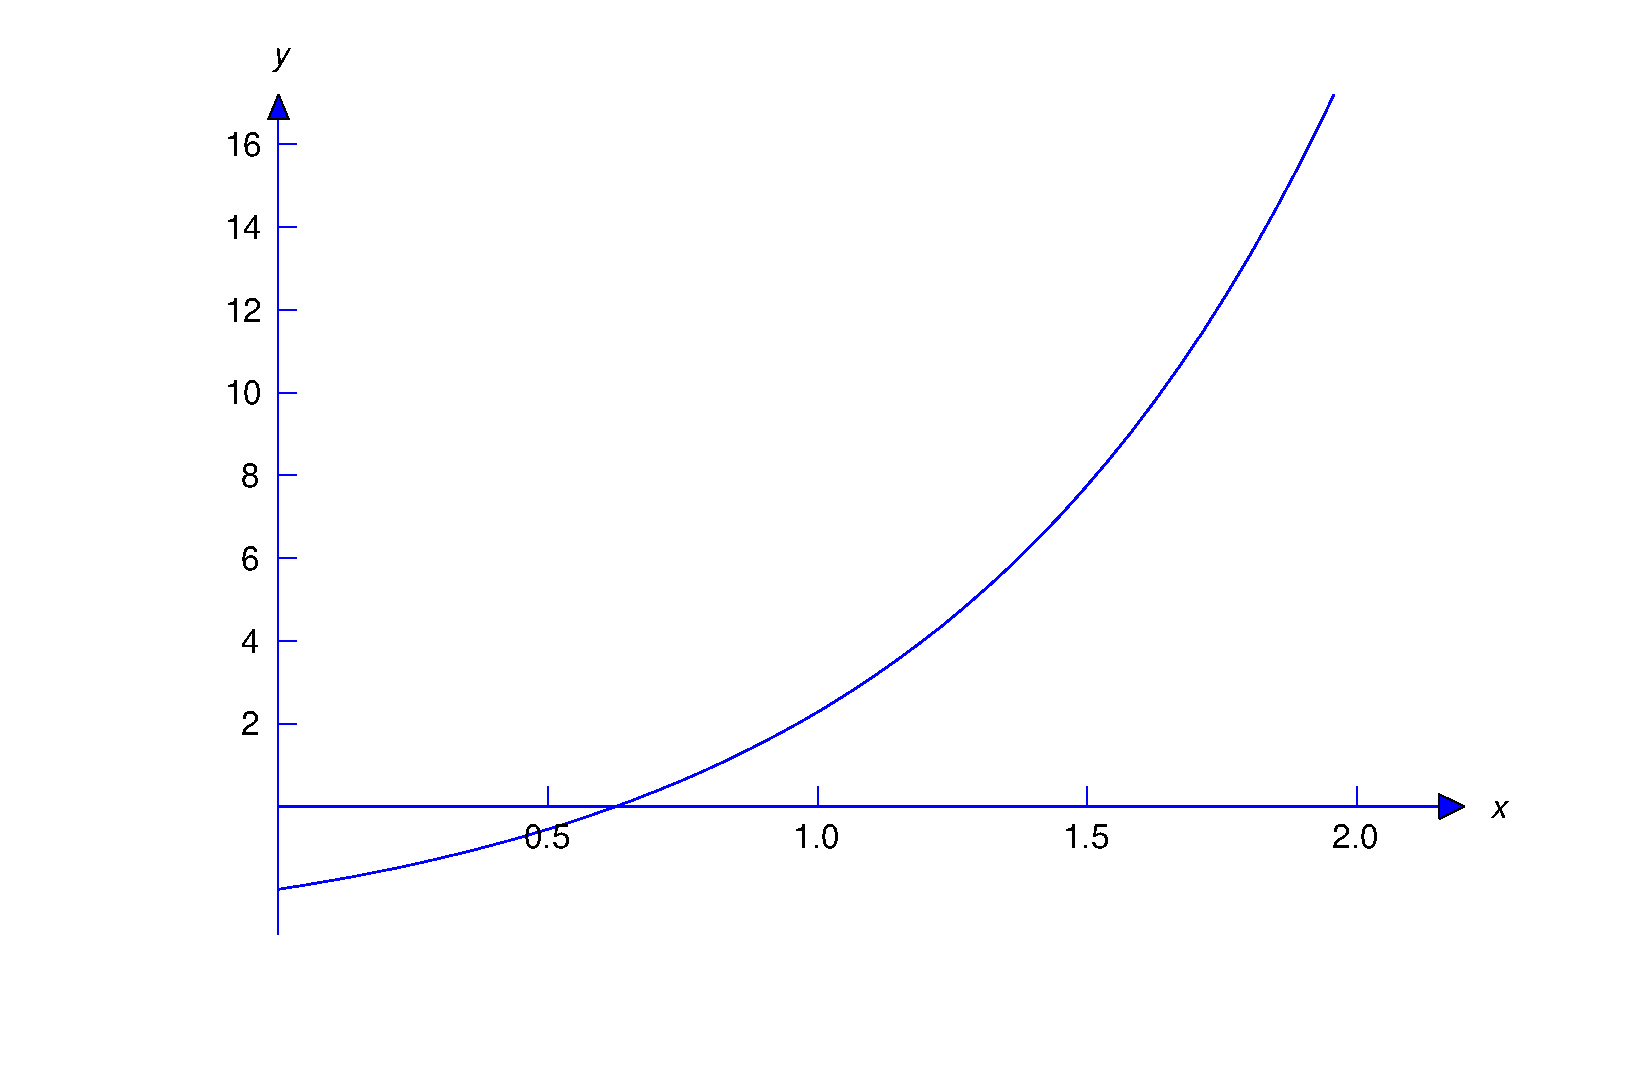
\includegraphics[bb=-78 148 689 643, width=5.67in, height=3.66in, keepaspectratio]{fig050302}
  \color{blue}
  \caption{$y=1+3x+x^{2}-e^{x}(3-x)$}
  \label{figure:5.3.2}
\end{figure}

\begin{example}
  \label{example:5.3.3} \rm Find the general solution of
  \begin{equation}
    \label{eq:5.3.13}x^{2}y''+xy'-4y=2x^{4}
  \end{equation}
  on $(-\infty,0)$ and $(0,\infty)$.
\end{example}

\solution In Example~\ref{example:5.1.3}, we verified that $y_{1}=x^{2}$ and $y_{2}=1/x^{2}$ form a
fundamental set of solutions of the complementary equation
\[
  x^{2}y''+xy'-4y=0
\]
on $(-\infty,0)$ and $(0,\infty)$. To find a particular solution of \eqref{eq:5.3.13}, we note that
if $y_{p}=Ax^{4}$, where $A$ is a constant then both sides of \eqref{eq:5.3.13} will be constant
multiples of $x^{4}$ and we may be able to choose $A$ so the two sides are equal. This is true in
this example, since if $y_{p}=Ax^{4}$ then
\[
  x^{2}y_{p}''+xy_{p}'-4y_{p}=x^{2}(12Ax^{2})+x(4Ax^{3})-4Ax^{4}=12Ax^{4}=2x^{4}
\]
if $A=1/6$; therefore, $y_{p}=x^{4}/6$ is a particular solution of \eqref{eq:5.3.13} on
$(-\infty,\infty)$. Theorem~\ref{thmtype:5.3.2} implies that the general solution of
\eqref{eq:5.3.13} on $(-\infty,0)$ and $(0,\infty)$ is
\[
  y=\frac{x^{4}}{6}+c_{1}x^{2}+\frac{c_{2}}{x^{2}}.
\]

\boxit{The Principle of Superposition}

\noindent
The next theorem enables us to break a nonhomogeneous equation into simpler parts, find a particular
solution for each part, and then combine their solutions to obtain a particular solution of the
original problem.

\begin{theorem}
  \color{blue}
  $[$The Principle of Superposition$]$ \label{thmtype:5.3.3} Suppose $y_{p_{1}}$ is a particular
  solution of
  \[
    y''+p(x)y'+q(x)y=f_{1}(x)
  \]
  on $(a,b)$ and $y_{p_{2}}$ is a particular solution of
  \[
    y''+p(x)y'+q(x)y=f_{2}(x)
  \]
  on $(a,b)$. Then
  \[
    y_{p}=y_{p_{1}}+y_{p_{2}}
  \]
  is a particular solution of
  \[
    y''+p(x)y'+q(x)y=f_{1}(x)+f_{2}(x)
  \]
  on $(a,b)$.
\end{theorem}

\proof If $y_{p}=y_{p_{1}}+y_{p_{2}}$ then
\begin{eqnarray*}
  y_{p}''+p(x)y_{p}'+q(x)y_{p} & = & (y_{p_{1}}+y_{p_{2}})''+p(x)(y_{p_{1}}+y_{p_{2}})'+q(x)(y_{p_{1}}+y_{p_{2}})                                \\
                               & = & \left(y_{p_{1}}''+p(x)y_{p_{1}}'+q(x)y_{p_{1}}\right)+\left(y_{p_{2}}''+p(x)y_{p_{2}}'+q(x)y_{p_{2}}\right) \\
                               & = & f_{1}(x)+f_{2}(x).\bbox
\end{eqnarray*}

It's easy to generalize Theorem~\ref{thmtype:5.3.3} to the equation
\begin{equation}
  \label{eq:5.3.14}y''+p(x)y'+q(x)y=f(x)
\end{equation}
where
\[
  f=f_{1}+f_{2}+\cdots+f_{k};
\]
thus, if $y_{p_{i}}$ is a particular solution of
\[
  y''+p(x)y'+q(x)y=f_{i}(x)
\]
on $(a,b)$ for $i=1$, $2$, \dots, $k$, then $y_{p_{1}}+y_{p_{2}}+\cdots+y_{p_{k}}$ is a particular
solution of \eqref{eq:5.3.14} on $(a,b)$. Moreover, by a proof similar to the proof of
Theorem~\ref{thmtype:5.3.3} we can formulate the principle of superposition in terms of a linear
equation written in the form
\[
  P_{0}(x)y''+P_{1}(x)y'+P_{2}(x)y=F(x)
\]
(Exercise~\ref{exer:5.3.39}); that is, if $y_{p_{1}}$ is a particular solution of
\[
  P_{0}(x)y''+P_{1}(x)y'+P_{2}(x)y=F_{1}(x)
\]
on $(a,b)$ and $y_{p_{2}}$ is a particular solution of
\[
  P_{0}(x)y''+P_{1}(x)y'+P_{2}(x)y=F_{2}(x)
\]
on $(a,b)$, then $y_{p_{1}}+y_{p_{2}}$ is a solution of
\[
  P_{0}(x)y''+P_{1}(x)y'+P_{2}(x)y=F_{1}(x)+F_{2}(x)
\]
on $(a,b)$.

\begin{example}
  \label{example:5.3.4} \rm The function $y_{p_{1}}=x^{4}/15$ is a particular solution of
  \begin{equation}
    \label{eq:5.3.15}x^{2}y''+4xy'+2y=2x^{4}
  \end{equation}
  on $(-\infty,\infty)$ and $y_{p_{2}}=x^{2}/3$ is a particular solution of
  \begin{equation}
    \label{eq:5.3.16}x^{2}y''+4xy'+2y=4x^{2}
  \end{equation}
  on $(-\infty,\infty)$. Use the principle of superposition to find a particular solution of
  \begin{equation}
    \label{eq:5.3.17}x^{2}y''+4xy'+2y=2x^{4}+4x^{2}
  \end{equation}
  on $(-\infty,\infty)$.
\end{example}

\solution The right side $F(x)=2x^{4}+4x^{2}$ in \eqref{eq:5.3.17} is the sum of the right sides
\[
  F_{1}(x)=2x^{4}\quad\mbox{ and }\quad F_{2}(x)=4x^{2}.
\]
in \eqref{eq:5.3.15} and \eqref{eq:5.3.16}. Therefore the principle of superposition implies that
\[
  y_{p}=y_{p_{1}}+y_{p_{2}}=\frac{x^{4}}{15}+\frac{x^{2}}{3}
\]
is a particular solution of \eqref{eq:5.3.17}.

\exercises

\noindent
In Exercises~\ref{exer:5.3.1}--\ref{exer:5.3.6} find a particular solution by the method used in
Example~\ref{example:5.3.2}. Then find the general solution and, where indicated, solve the initial
value problem and graph the solution.

\begin{exerciselist}
  \item\label{exer:5.3.1} $y''+5y'-6y=22+18x-18x^{2}$

  \item\label{exer:5.3.2} $y''-4y'+5y=1+5x$

  \item\label{exer:5.3.3} $y''+8y'+7y=-8-x+24x^{2}+7x^{3}$

  \item\label{exer:5.3.4} $y''-4y'+4y=2+8x-4x^{2}$

  \item\label{exer:5.3.5} \CGex $y''+2y'+10y=4+26x+6x^{2}+10x^{3},\quad y(0)=2, \quad y'(0)=9$

  \item\label{exer:5.3.6} \CGex $y''+6y'+10y=22+20x,\quad y(0)=2,\; y'(0)=-2$

  \item\label{exer:5.3.7} Show that the method used in Example~\ref{example:5.3.2} won't yield a
        particular solution of
  \[
    y''+y'=1+2x+x^{2}; \eqno{\rm(A)}
  \]
  that is, (A) doesn't have a particular solution of the form $y_{p}=A+Bx+Cx^{2}$, where $A$, $B$,
  and $C$ are constants.

  \exercisetext{In Exercises~\ref{exer:5.3.8}--\ref{exer:5.3.13} find a particular solution by the
  method used in Example~\ref{example:5.3.3}.}

  \begin{tabular}[t]{@{}p{168pt}@{}p{168pt}}
    \item\label{exer:5.3.8} $x^{2}y''+7xy'+8y=\dst\frac{6}{x}$ &
    \item\label{exer:5.3.9} $x^{2}y''-7xy'+7y=13x^{1/2}$
  \end{tabular}

  \begin{tabular}[t]{@{}p{168pt}@{}p{168pt}}
    \item\label{exer:5.3.10} $x^{2}y''-xy'+y=2x^{3}$ &
    \item\label{exer:5.3.11} $x^{2}y''+5xy'+4y=\dst\frac{1}{x^{3}}$
  \end{tabular}

  \begin{tabular}[t]{@{}p{168pt}@{}p{168pt}}
    \item\label{exer:5.3.12} $x^{2}y''+xy'+y=10x^{1/3}$ &
    \item\label{exer:5.3.13} $x^{2}y''-3xy'+13y=2x^{4}$
  \end{tabular}

  \item\label{exer:5.3.14} Show that the method suggested for finding a particular solution in
        Exercises~\ref{exer:5.3.8}-\ref{exer:5.3.13} won't yield a particular solution of
  \[
    x^{2}y''+3xy'-3y=\frac{1}{x^{3}}; \eqno{\rm(A)}
  \]
  that is, (A) doesn't have a particular solution of the form $y_{p}=A/x^{3}$.

  \item\label{exer:5.3.15} Prove: If $a$, $b$, $c$, $\alpha$, and $M$ are constants and $M\ne0$ then
  \[
    ax^{2}y''+bxy'+cy=Mx^{\alpha}
  \]
  has a particular solution $y_{p}=Ax^{\alpha}$ ($A=$ constant) if and only if
  $a\alpha(\alpha-1)+b\alpha+c\ne0$.

  \exercisetext{If $a$, $b$, $c$, and $\alpha$ are constants, then \[a(e^{\alpha x})''+b(e^{\alpha
  x})'+ce^{\alpha x}=(a\alpha^{2}+b\alpha+c)e^{\alpha x}.\] Use this in
  Exercises~\ref{exer:5.3.16}--\ref{exer:5.3.21} to find a particular solution . Then find the
  general solution and, where indicated, solve the initial value problem and graph the solution.}
  %Exercises~\ref{exer:5.3.16}--\ref{exer:5.3.21} are referenced later as
  %\exercisec.

  \begin{tabular}[t]{@{}p{168pt}@{}p{168pt}}
    \item\label{exer:5.3.16} $y''+5y'-6y=6e^{3x}$ & \vspace*{10pt}
    \item\label{exer:5.3.17} $y''-4y'+5y=e^{2x}$
  \end{tabular}

  \item\label{exer:5.3.18} \CGex $y''+8y'+7y=10e^{-2x},\quad y(0)=-2,\; y'(0)=10$

  \item\label{exer:5.3.19} \CGex $y''-4y'+4y=e^{x},\quad y(0)=2,\quad y'(0)=0$

  \begin{tabular}[t]{@{}p{168pt}@{}p{168pt}}
    \item\label{exer:5.3.20} $y''+2y'+10y=e^{x/2}$ &
    \item\label{exer:5.3.21} $y''+6y'+10y=e^{-3x}$
  \end{tabular}

  \item\label{exer:5.3.22} Show that the method suggested for finding a particular solution in
        Exercises~\ref{exer:5.3.16}-\ref{exer:5.3.21} won't yield a particular solution of
  \[
    y''-7y'+12y=5e^{4x}; \eqno{\rm(A)}
  \]
  that is, (A) doesn't have a particular solution of the form $y_{p}=Ae^{4x}$.

  \item\label{exer:5.3.23} Prove: If $\alpha$ and $M$ are constants and $M\ne0$ then constant
        coefficient equation
  \[
    ay''+by'+cy=Me^{\alpha x}
  \]
  has a particular solution $y_{p}=Ae^{\alpha x}$ ($A=$ constant) if and only if $e^{\alpha x}$
  isn't a solution of the complementary equation.

  \exercisetext{If $\omega$ is a constant, differentiating a linear combination of $\cos\omega x$
  and $\sin\omega x$ with respect to $x$ yields another linear combination of $\cos\omega x$ and
  $\sin\omega x$. In Exercises~\ref{exer:5.3.24}--\ref{exer:5.3.29} use this to find a particular
  solution of the equation. Then find the general solution and, where indicated, solve the initial
  value problem and graph the solution.}

  \item\label{exer:5.3.24} $y''-8y'+16y=23\cos x-7\sin x$

  \item\label{exer:5.3.25} $y''+y'=-8\cos2x+6\sin2x$

  \item\label{exer:5.3.26} $y''-2y'+3y=-6\cos3x+6\sin3x$

  \item\label{exer:5.3.27}$y''+6y'+13y=18\cos x+6\sin x$

  \item\label{exer:5.3.28} \CGex $y''+7y'+12y=-2\cos2x+36\sin2x,\quad y(0)=-3,\quad y'(0)=3$

  \item\label{exer:5.3.29} \CGex $y''-6y'+9y=18\cos3x+18\sin3x,\quad y(0)=2,\quad y'(0)=2$

  \item\label{exer:5.3.30} Find the general solution of
  \[
    y''+\omega_{0}^{2}y=M\cos\omega x+N\sin\omega x,
  \]
  where $M$ and $N$ are constants and $\omega$ and $\omega_{0}$ are distinct positive numbers.

  \item\label{exer:5.3.31} Show that the method suggested for finding a particular solution in
        Exercises~\ref{exer:5.3.24}-\ref{exer:5.3.29} won't yield a particular solution of
  \[
    y''+y=\cos x+\sin x; \eqno{\rm(A)}
  \]
  that is, (A) does not have a particular solution of the form $y_{p}=A\cos x+B\sin x$.

  \item\label{exer:5.3.32} Prove: If $M$, $N$ are constants (not both zero) and $\omega>0$, the
        constant coefficient equation
  \[
    ay''+by'+cy=M\cos\omega x+N\sin\omega x \eqno{\rm(A)}
  \]
  has a particular solution that's a linear combination of $\cos\omega x$ and $\sin\omega x$ if and
  only if the left side of (A) is not of the form $a(y''+\omega^{2}y)$, so that $\cos\omega x$ and
  $\sin\omega x$ are solutions of the complementary equation.

  \exercisetext{In Exercises~\ref{exer:5.3.33}--\ref{exer:5.3.38} refer to the cited exercises and
  use the principal of superposition to find a particular solution. Then find the general solution.}

  \item\label{exer:5.3.33} $y''+5y'-6y=22+18x-18x^{2}+6e^{3x}$ (See Exercises~\ref{exer:5.3.1} and
        \ref{exer:5.3.16}.)

  \item\label{exer:5.3.34} $y''-4y'+5y=1+5x+e^{2x}$ (See Exercises~\ref{exer:5.3.2} and
        \ref{exer:5.3.17}.)

  \item\label{exer:5.3.35} $y''+8y'+7y=-8-x+24x^{2}+7x^{3}+10e^{-2x}$ (See
        Exercises~\ref{exer:5.3.3} and \ref{exer:5.3.18}.)

  \item\label{exer:5.3.36} $y''-4y'+4y=2+8x-4x^{2}+e^{x}$ (See Exercises~\ref{exer:5.3.4} and
        \ref{exer:5.3.19}.)

  \item\label{exer:5.3.37} $y''+2y'+10y=4+26x+6x^{2}+10x^{3}+e^{x/2}$ (See
        Exercises~\ref{exer:5.3.5} and \ref{exer:5.3.20}.)

  \item\label{exer:5.3.38} $y''+6y'+10y=22+20x+e^{-3x}$ (See Exercises~\ref{exer:5.3.6} and
        \ref{exer:5.3.21}.)

  \item\label{exer:5.3.39} Prove: If $y_{p_{1}}$ is a particular solution of
  \[
    P_{0}(x)y''+P_{1}(x)y'+P_{2}(x)y=F_{1}(x)
  \]
  on $(a,b)$ and $y_{p_{2}}$ is a particular solution of
  \[
    P_{0}(x)y''+P_{1}(x)y'+P_{2}(x)y=F_{2}(x)
  \]
  on $(a,b)$, then $y_{p}=y_{p_{1}}+y_{p_{2}}$ is a solution of
  \[
    P_{0}(x)y''+P_{1}(x)y'+P_{2}(x)y=F_{1}(x)+F_{2}(x)
  \]
  on $(a,b)$.

  \item\label{exer:5.3.40} Suppose $p$, $q$, and $f$ are continuous on $(a,b)$. Let $y_{1}$,
        $y_{2}$, and $y_{p}$ be twice differentiable on $(a,b)$, such that
        $y=c_{1}y_{1}+c_{2}y_{2}+y_{p}$ is a solution of
  \[
    y''+p(x)y'+q(x)y=f
  \]
  on $(a,b)$ for every choice of the constants $c_{1}$, $c_{2}$. Show that $y_{1}$ and $y_{2}$ are
  solutions of the complementary equation on $(a,b)$.
\end{exerciselist}


\section{The Method of Undetermined Coefficients I}

\noindent
In this section we consider the constant coefficient equation
\begin{equation} \label{eq:5.4.1}
ay''+by'+cy=e^{\alpha x}G(x),
\end{equation}
where $\alpha$ is a constant and $G$ is a polynomial.

From Theorem~\ref{thmtype:5.3.2}, the general solution of (\ref{eq:5.4.1})
is
$y=y_p+c_1y_1+c_2y_2$, where $y_p$ is a particular solution of
(\ref{eq:5.4.1}) and $\{y_1,y_2\}$ is a fundamental set of
solutions of the complementary equation
$$
ay''+by'+cy=0.
$$
In Section~5.2 we showed how to find $\{y_1,y_2\}$. In this
section we'll show how to find $y_p$. The procedure that we'll use
is called {\color{blue}\it the method of undetermined coefficients\/}.

Our first example is similar to
Exercises~\ref{exer:5.3.16}--\ref{exer:5.3.21}.

\begin{example}\label{example:5.4.1} \rm
Find a particular solution of
\begin{equation} \label{eq:5.4.2}
y''-7y'+12y=4e^{2x}.
\end{equation}
Then find the general solution.
\end{example}

\solution
Substituting $y_p=Ae^{2x}$ for $y$ in (\ref{eq:5.4.2}) will produce a
constant multiple of $Ae^{2x}$ on the left side of (\ref{eq:5.4.2}), so it
may be possible to choose $A$ so that $y_p$ is a solution of
(\ref{eq:5.4.2}). Let's try it;   if $y_p=Ae^{2x}$ then
$$
y_p''-7y_p'+12y_p=4Ae^{2x}-14Ae^{2x}+12Ae^{2x}=2Ae^{2x}=4e^{2x}
$$
if $A=2$. Therefore $y_p=2e^{2x}$ is a particular solution of
(\ref{eq:5.4.2}). To find the general solution, we note that the
characteristic polynomial of the complementary equation
\begin{equation} \label{eq:5.4.3}
y''-7y'+12y=0
\end{equation}
is $p(r)=r^2-7r+12=(r-3)(r-4)$, so $\{e^{3x},e^{4x}\}$ is a
fundamental set of solutions of (\ref{eq:5.4.3}). Therefore the general
solution of (\ref{eq:5.4.2}) is
$$
 y=2e^{2x}+c_1e^{3x}+c_2e^{4x}.
$$

\begin{example}\label{example:5.4.2} \rm
Find a particular solution of
\begin{equation} \label{eq:5.4.4}
y''-7y'+12y=5e^{4x}.
\end{equation}
Then find the general solution.
\end{example}

\solution
Fresh from our success in finding a particular solution of
(\ref{eq:5.4.2}) --- where we chose $y_p=Ae^{2x}$ because the right side
of
(\ref{eq:5.4.2}) is a constant multiple of $e^{2x}$ --- it may seem
reasonable to try $y_p=Ae^{4x}$ as a particular solution of
(\ref{eq:5.4.4}). However, this won't work, since we saw in
Example~\ref{example:5.4.1} that $e^{4x}$ is a solution of the
complementary equation (\ref{eq:5.4.3}), so substituting $y_p=Ae^{4x}$
into the left side of (\ref{eq:5.4.4}) produces zero on the left, no
matter how we choose$A$. To discover a suitable form for $y_p$,
we use the same approach that we used in Section~5.2 to find a
second solution of
$$
ay''+by'+cy=0
$$
in the case where the characteristic equation has a repeated real
root: we look for solutions of (\ref{eq:5.4.4}) in the form $y=ue^{4x}$,
where $u$ is a function to be determined. Substituting
\begin{equation} \label{eq:5.4.5}
y=ue^{4x},\quad
y'=u'e^{4x}+4ue^{4x},\mbox{\quad and \quad}
y''=u''e^{4x}+8u'e^{4x}+16ue^{4x}
\end{equation}
into (\ref{eq:5.4.4}) and canceling the common factor $e^{4x}$ yields
$$
(u''+8u'+16u)-7(u'+4u)+12u=5,
$$
or
$$
u''+u'=5.
$$
By inspection we  see that $u_p=5x$ is a particular solution of
this equation, so $y_p=5xe^{4x}$ is a particular solution of
(\ref{eq:5.4.4}). Therefore
$$
y=5xe^{4x}+c_1e^{3x}+c_2e^{4x}
$$
is the general solution.

\begin{example}\label{example:5.4.3} \rm
Find a particular solution of
\begin{equation} \label{eq:5.4.6}
y''-8y'+16y=2e^{4x}.
\end{equation}
\end{example}

\solution
Since the characteristic polynomial of the complementary equation
\begin{equation} \label{eq:5.4.7}
y''-8y'+16y=0
\end{equation}
is $p(r)=r^2-8r+16=(r-4)^2$, both $y_1=e^{4x}$ and $y_2=xe^{4x}$ are
solutions of (\ref{eq:5.4.7}). Therefore (\ref{eq:5.4.6}) does not have a
solution of the form $y_p=Ae^{4x}$ or $y_p=Axe^{4x}$. As in
Example~\ref{example:5.4.2}, we look for solutions of (\ref{eq:5.4.6}) in the
form $y=ue^{4x}$, where $u$ is a function to be determined.
Substituting from (\ref{eq:5.4.5}) into (\ref{eq:5.4.6}) and canceling the
common factor $e^{4x}$ yields
$$
(u''+8u'+16u)-8(u'+4u)+16u=2,
$$
or
$$
u''=2.
$$
Integrating twice and taking the constants of integration to be zero
shows that $u_p=x^2$ is a particular solution of this equation, so
$y_p=x^2e^{4x}$ is a particular solution of (\ref{eq:5.4.4}). Therefore
$$
y=e^{4x}(x^2+c_1+c_2x)
$$
is the general solution. \bbox

The preceding examples illustrate the following facts concerning
the form of a particular solution $y_p$
of a constant coefficent equation
$$
ay''+by'+cy=ke^{\alpha x},
$$
where $k$ is a nonzero constant:

\medskip

\begin{alist}
\item % (a)
If $e^{\alpha x}$ isn't  a solution of the complementary
equation
\begin{equation} \label{eq:5.4.8}
ay''+by'+cy=0,
\end{equation}
then  $y_p=Ae^{\alpha x}$, where $A$ is a constant. (See
Example~\ref{example:5.4.1}).
\item % (b)
If $e^{\alpha x}$ is a solution of (\ref{eq:5.4.8}) but $xe^{\alpha x}$
is not, then  $y_p=Axe^{\alpha x}$,  where $A$ is a constant.
(See Example~\ref{example:5.4.2}.)
\item % (c)
If both $e^{\alpha x}$ and $xe^{\alpha x}$ are solutions of (\ref{eq:5.4.8}),
then  $y_p=Ax^2e^{\alpha x}$,  where $A$ is a constant.
(See Example~\ref{example:5.4.3}.)
\end{alist}
See Exercise~\ref{exer:5.4.30}  for the proofs of these facts.

In all three cases you can just substitute the appropriate form for
$y_p$ and its derivatives directly into
$$
ay_p''+by_p'+cy_p=ke^{\alpha x},
$$
and solve for the constant $A$, as we did in
Example~\ref{example:5.4.1}.
 (See Exercises~\ref{exer:5.4.31}--\ref{exer:5.4.33}.)
However, if the equation is
$$
ay''+by'+cy=k e^{\alpha x}G(x),
$$
where $G$ is a polynomial of degree greater than zero, we recommend
that you use the substitution $y=ue^{\alpha x}$ as we did in
Examples~\ref{example:5.4.2} and \ref{example:5.4.3}. The equation for $u$
will turn out to be
\begin{equation} \label{eq:5.4.9}
au''+p'(\alpha)u'+p(\alpha)u=G(x),
\end{equation}
where $p(r)=ar^2+br+c$ is the characteristic polynomial of the
complementary equation and $p'(r)=2ar+b$ (Exercise~\ref{exer:5.4.30});
however, you shouldn't memorize this since it's easy to derive the
equation for $u$ in any particular case. Note, however, that if
$e^{\alpha x}$ is a solution of the complementary equation then
$p(\alpha)=0$, so (\ref{eq:5.4.9}) reduces to
$$
au''+p'(\alpha)u'=G(x),
$$
while if both $e^{\alpha x}$ and $xe^{\alpha x}$ are solutions of the
complementary equation then $p(r)=a(r-\alpha)^2$ and
$p'(r)=2a(r-\alpha)$, so $p(\alpha)=p'(\alpha)=0$ and (\ref{eq:5.4.9})
reduces to
$$
au''=G(x).
$$

\begin{example}\label{example:5.4.4} \rm
Find a particular solution of
\begin{equation} \label{eq:5.4.10}
y''-3y'+2y=e^{3x}(-1+2x+x^2).
\end{equation}
\end{example}

\solution
Substituting
$$
y=ue^{3x},\quad y'=u'e^{3x}+3ue^{3x},\mbox{\quad and }
y''=u''e^{3x}+6u'e^{3x}+9ue^{3x}
$$
into (\ref{eq:5.4.10}) and  canceling $e^{3x}$  yields
$$
(u''+6u'+9u)-3(u'+3u)+2u=-1+2x+x^2,
$$
or
\begin{equation} \label{eq:5.4.11}
u''+3u'+2u=-1+2x+x^2.
\end{equation}
As in Example~\ref{exer:5.3.2}, in order to guess a form for a particular
solution of
(\ref{eq:5.4.11}), we note that substituting a second degree polynomial
$u_p=A+Bx+Cx^2$ for $u$ in the left side of (\ref{eq:5.4.11}) produces
another second degree polynomial with coefficients that depend upon
$A$, $B$, and $C$;   thus,
$$
\mbox{ if \quad}u_p=A+Bx+Cx^2\mbox{\quad then \quad}
u_p'=B+2Cx\mbox{\quad and \quad} u_p''=2C.
$$
If $u_p$ is to satisfy (\ref{eq:5.4.11}),  we must have
\begin{eqnarray*}
u_p''+3u_p'+2u_p&=&2C+3(B+2Cx)+2(A+Bx+Cx^2)\\
&=&(2C+3B+2A)+(6C+2B)x+2Cx^2=-1+2x+x^2.
\end{eqnarray*}
Equating  coefficients of like powers of $x$ on the two sides of the
last equality yields
$$
\begin{array}{rcr}
2C&=&1\phantom{.}\\
2B+6C&=&2\phantom{.}\\
2A+3B+2C&=& -1.
\end{array}
$$
Solving these equations for $C$, $B$, and $A$ (in that order) yields
 $C=1/2,B=-1/2,A=-1/4$.  Therefore
$$
u_p=-{1\over4}(1+2x-2x^2)
$$
is a particular solution of  (\ref{eq:5.4.11}), and
$$
y_p=u_pe^{3x}=-{e^{3x}\over4}(1+2x-2x^2)
$$
is a particular solution of  (\ref{eq:5.4.10}).

\begin{example}\label{example:5.4.5} \rm
 Find a particular solution of
\begin{equation} \label{eq:5.4.12}
y''-4y'+3y=e^{3x}(6+8x+12x^2).
\end{equation}
\end{example}

\solution
Substituting
$$
y=ue^{3x},\quad y'=u'e^{3x}+3ue^{3x},\mbox{\quad and }
y''=u''e^{3x}+6u'e^{3x}+9ue^{3x}
$$
into (\ref{eq:5.4.12}) and  canceling $e^{3x}$  yields
$$
(u''+6u'+9u)-4(u'+3u)+3u=6+8x+12x^2,
$$
or
\begin{equation} \label{eq:5.4.13}
u''+2u'=6+8x+12x^2.
\end{equation}
There's no $u$ term in this equation, since $e^{3x}$ is a solution of
the complementary equation for (\ref{eq:5.4.12}). (See
Exercise~\ref{exer:5.4.30}.) Therefore (\ref{eq:5.4.13}) does not have a
particular solution of the form $u_p=A+Bx+Cx^2$ that we used
successfully in Example~\ref{example:5.4.4}, since with this choice of
$u_p$,
$$
u_p''+2u_p'=2C+(B+2Cx)
$$
can't contain the last term ($12x^2$) on the right side of
(\ref{eq:5.4.13}). Instead, let's try $u_p=Ax+Bx^2+Cx^3$ on the grounds
that
$$
u_p'=A+2Bx+3Cx^2\mbox{\quad and \quad}
u_p''=2B+6Cx
$$
together contain all the powers of $x$ that appear on the right side
of (\ref{eq:5.4.13}).

Substituting these expressions in place of $u'$ and $u''$  in
(\ref{eq:5.4.13}) yields
$$
(2B+6Cx)+2(A+2Bx+3Cx^2)=(2B+2A)+(6C+4B)x+6Cx^2=6+8x+12x^2.
$$
Comparing coefficients of like powers of $x$ on the two sides of the
last equality shows that $u_p$ satisfies (\ref{eq:5.4.13}) if
$$
\begin{array}{rcr}
6C&=&12\phantom{.}\\
4B+6C&=&8\phantom{.}\\
2A+2B\phantom{+6u_2}&=&6.
\end{array}
$$
Solving these equations successively yields $C=2$, $B=-1$, and $A=4$.
Therefore
$$
u_p=x(4-x+2x^2)
$$
is a particular solution of  (\ref{eq:5.4.13}),
and
$$
y_p=u_pe^{3x}=xe^{3x}(4-x+2x^2)
$$
is a particular solution of  (\ref{eq:5.4.12}).

\begin{example}\label{example:5.4.6} \rm
Find a particular solution of
\begin{equation} \label{eq:5.4.14}
4y''+4y'+y=e^{-x/2}(-8+48x+144x^2).
\end{equation}
\end{example}

\solution  Substituting
$$
y=ue^{-x/2},\quad  y'=u'e^{-x/2}-{1\over2}ue^{-x/2},\mbox{\quad and
\quad} y''=u''e^{-x/2}-u'e^{-x/2}+{1\over4}ue^{-x/2}
$$
into (\ref{eq:5.4.14}) and  canceling $e^{-x/2}$  yields
$$
4\left(u''-u'+{u\over4}\right)+4\left(u'-{u\over2}\right)+u=4u''=-8+48x+144x^2,
$$
or
\begin{equation} \label{eq:5.4.15}
u''=-2+12x+36x^2,
\end{equation}
which does not contain $u$ or $u'$ because $e^{-x/2}$ and $xe^{-x/2}$
are both solutions of the complementary equation. (See
Exercise~\ref{exer:5.4.30}.) To obtain a particular solution of
(\ref{eq:5.4.15}) we integrate twice, taking the constants of integration
to be zero;   thus,
$$
u_p'=-2x+6x^2+12x^3\mbox{\quad and \quad}
u_p=-x^2+2x^3+3x^4=x^2(-1+2x+3x^2).
$$
Therefore
$$
y_p=u_pe^{-x/2}=x^2e^{-x/2}(-1+2x+3x^2)
$$
is a particular solution of  (\ref{eq:5.4.14}).

\boxit{Summary}

\noindent
The preceding examples illustrate the following facts concerning
 particular solutions of a constant coefficent equation of the form
$$
ay''+by'+cy=e^{\alpha x}G(x),
$$
where $G$ is a polynomial (see Exercise~\ref{exer:5.4.30}):
\begin{alist}
\item % (a)
If $e^{\alpha x}$ isn't  a solution of the complementary
equation
\begin{equation} \label{eq:5.4.16}
ay''+by'+cy=0,
\end{equation}
then  $y_p=e^{\alpha x}Q(x)$,
 where $Q$ is a polynomial of the same degree as $G$.
(See Example~\ref{example:5.4.4}).
\item % (b)
If $e^{\alpha x}$ is a solution of (\ref{eq:5.4.16}) but $xe^{\alpha x}$
is not, then  $y_p=xe^{\alpha x}Q(x)$,
 where $Q$ is a polynomial of the same degree as $G$.
(See Example~\ref{example:5.4.5}.)
\item % (c)
If both $e^{\alpha x}$ and $xe^{\alpha x}$ are solutions of (\ref{eq:5.4.16}),
then  $y_p=x^2e^{\alpha x}Q(x)$,
 where $Q$ is a polynomial of the same degree as $G$.
(See Example~\ref{example:5.4.6}.)
\end{alist}

In all three cases, you can just substitute the appropriate form for
$y_p$ and its derivatives directly into
$$
ay_p''+by_p'+cy_p=e^{\alpha x}G(x),
$$
and solve for the coefficients of the polynomial $Q$. However, if you
try this you will see that the computations are more tedious than
those that you encounter by making the substitution $y=ue^{\alpha x}$
and finding a particular solution of the resulting equation for $u$.
(See Exercises~\ref{exer:5.4.34}-\ref{exer:5.4.36}.) In Case~\part{a}
the equation for $u$ will be of the form
$$
au''+p'(\alpha)u'+p(\alpha)u=G(x),
$$
with a particular solution of the form $u_p=Q(x)$, a polynomial of the
same degree as $G$, whose coefficients can be found by the method used
in Example~\ref{example:5.4.4}. In Case~\part{b}  the equation for
$u$ will be of the form
$$
au''+p'(\alpha)u'=G(x)
$$
(no $u$ term on the left), with a particular solution of the form
$u_p=xQ(x)$, where $Q$ is a polynomial of the same degree as $G$ whose
coefficents can be found by the method used in
Example~\ref{example:5.4.5}. In Case~\part{c}  the equation for $u$
will be of the form
$$
au''=G(x)
$$
with a particular solution of the form $u_p=x^2Q(x)$ that can be
obtained by integrating $G(x)/a$ twice and taking the constants of
integration to be zero, as in Example~\ref{example:5.4.6}.

\boxit{Using the Principle of Superposition}

\noindent
The next example shows how to combine the method of undetermined
coefficients and Theorem~\ref{thmtype:5.3.3}, the principle of
superposition.

\begin{example}\label{example:5.4.7} \rm
Find a particular solution of
\begin{equation} \label{eq:5.4.17}
y''-7y'+12y=4e^{2x}+5e^{4x}.
\end{equation}
\end{example}

\solution
In Example~\ref{example:5.4.1} we found that $y_{p_1}=2e^{2x}$
is a particular solution of
$$
y''-7y'+12y=4e^{2x},
$$
and in Example~\ref{example:5.4.2} we found that $y_{p_2}=5xe^{4x}$
is a particular solution of
$$
y''-7y'+12y=5e^{4x}.
$$
Therefore the principle of superposition implies that
$y_p=2e^{2x}+5xe^{4x}$ is a particular solution of (\ref{eq:5.4.17}).

\exercises
In Exercises \ref{exer:5.4.1}--\ref{exer:5.4.14} find a particular
solution.

\begin{exerciselist}

\begin{tabular}[t]{@{}p{168pt}@{}p{168pt}}
\item\label{exer:5.4.1} $y''-3y'+2y=e^{3x}(1+x)$
&\vspace*{10pt}  \item\label{exer:5.4.2} $y''-6y'+5y=e^{-3x}(35-8x)$
\end{tabular}

\begin{tabular}[t]{@{}p{168pt}@{}p{168pt}}
\item\label{exer:5.4.3} $y''-2y'-3y=e^x(-8+3x)$
&  \item\label{exer:5.4.4} $y''+2y'+y=e^{2x}(-7-15x+9x^2)$
\end{tabular}

\begin{tabular}[t]{@{}p{168pt}@{}p{168pt}}
\item\label{exer:5.4.5} $y''+4y=e^{-x}(7-4x+5x^2)$
&  \item\label{exer:5.4.6} $y''-y'-2y=e^x(9+2x-4x^2)$
\end{tabular}

\begin{tabular}[t]{@{}p{168pt}@{}p{168pt}}
\item\label{exer:5.4.7} $y''-4y'-5y=-6xe^{-x}$
&  \item\label{exer:5.4.8} $y''-3y'+2y=e^x(3-4x)$
\end{tabular}

\begin{tabular}[t]{@{}p{168pt}@{}p{168pt}}
\item\label{exer:5.4.9} $y''+y'-12y=e^{3x}(-6+7x)$
&  \item\label{exer:5.4.10} $2y''-3y'-2y=e^{2x}(-6+10x)$
\end{tabular}

\begin{tabular}[t]{@{}p{168pt}@{}p{168pt}}
\item\label{exer:5.4.11} $y''+2y'+y=e^{-x}(2+3x)$ &
\item\label{exer:5.4.12} $y''-2y'+y=e^x(1-6x)$
\end{tabular}

\item\label{exer:5.4.13} $y''-4y'+4y=e^{2x}(1-3x+6x^2)$

\item\label{exer:5.4.14} $9y''+6y'+y=e^{-x/3}(2-4x+4x^2)$

\exercisetext{In Exercises \ref{exer:5.4.15}--\ref{exer:5.4.19} find the general
solution.}

\begin{tabular}[t]{@{}p{168pt}@{}p{168pt}}
\item\label{exer:5.4.15} $y''-3y'+2y=e^{3x}(1+x)$ &
\vspace*{10pt}\item\label{exer:5.4.16} $y''-6y'+8y=e^x(11-6x)$
\end{tabular}

\begin{tabular}[t]{@{}p{168pt}@{}p{168pt}}
\item\label{exer:5.4.17} $ y''+6y'+9y=e^{2x}(3-5x)$ &
\item\label{exer:5.4.18} $y''+2y'-3y=-16xe^x$
\end{tabular}

\item\label{exer:5.4.19} $y''-2y'+y=e^x(2-12x)$

\newpage
\exercisetext{In Exercises \ref{exer:5.4.20}--\ref{exer:5.4.23} solve the
initial value problem and plot the solution.}

\item\label{exer:5.4.20} \CGex $y''-4y'-5y=9e^{2x}(1+x), \quad  y(0)=0,\quad y'(0)=-10$
\item\label{exer:5.4.21} \CGex $y''+3y'-4y=e^{2x}(7+6x), \quad  y(0)=2,\quad y'(0)=8$
\item\label{exer:5.4.22} \CGex $y''+4y'+3y=-e^{-x}(2+8x), \quad  y(0)=1,\quad y'(0)=2$
\item\label{exer:5.4.23} \CGex $y''-3y'-10y=7e^{-2x}, \quad  y(0)=1,\quad y'(0)=-17$

\exercisetext{In Exercises~\ref{exer:5.4.24}--\ref{exer:5.4.29} use
the principle of superposition to find a particular solution.}

\item\label{exer:5.4.24} $y''+y'+y=xe^x+e^{-x}(1+2x)$
\item\label{exer:5.4.25} $y''-7y'+12y=-e^x(17-42x)-e^{3x}$
\item\label{exer:5.4.26} $y''-8y'+16y=6xe^{4x}+2+16x+16x^2$
\item\label{exer:5.4.27} $y''-3y'+2y=-e^{2x}(3+4x)-e^x$
\item\label{exer:5.4.28} $y''-2y'+2y=e^x(1+x)+e^{-x}(2-8x+5x^2)$
\item\label{exer:5.4.29}
$y''+y=e^{-x}(2-4x+2x^2)+e^{3x}(8-12x-10x^2)$

\item\label{exer:5.4.30}
\begin{alist}
 \item % (a)
Prove that  $y$ is a solution of the constant coefficient equation
$$
ay''+by'+cy=e^{\alpha x}G(x)
\eqno{\rm (A)}
$$
if and only if $y=ue^{\alpha x}$, where $u$ satisfies
$$
au''+p'(\alpha)u'+p(\alpha)u=G(x)
\eqno{\rm (B)}
$$
and   $p(r)=ar^2+br+c$ is the characteristic polynomial of
the complementary equation
$$
ay''+by'+cy=0.
$$

For the rest of this exercise, let $G$ be
 a polynomial. Give the requested proofs for the case where
$$
G(x)=g_0+g_1x+g_2x^2+g_3x^3.
$$

\item % (b)
Prove that if $e^{\alpha x}$ isn't  a solution of the complementary
equation then (B) has a particular solution of the
form $u_p=A(x)$, where $A$ is a polynomial of the same degree as $G$,
as in Example~\ref{example:5.4.4}. Conclude that (A) has
a particular solution of the form $y_p=e^{\alpha x}A(x)$.

\item % (c)
Show that if $e^{\alpha x}$ is a solution of the complementary
equation and $xe^{\alpha x}$ isn't , then (B) has a
particular solution of the form $u_p=xA(x)$, where $A$ is a polynomial
of the same degree as $G$, as in Example~\ref{example:5.4.5}. Conclude
that (A) has a particular solution of the form
$y_p=xe^{\alpha x}A(x)$.

\item % (d)
Show that if $e^{\alpha x}$ and $xe^{\alpha x}$ are both solutions of
the complementary equation then (B) has a
particular solution of the form $u_p=x^2A(x)$, where $A$ is a
polynomial of the same degree as $G$, and $x^2A(x)$ can be obtained by
integrating $G/a$ twice, taking the constants of integration to be
zero, as in Example~\ref{example:5.4.6}. Conclude that
(A) has a particular solution of the form
$y_p=x^2e^{\alpha x}A(x)$.
\end{alist}

\exercisetext{Exercises~\ref{exer:5.4.31}--\ref{exer:5.4.36}
treat the equations considered in
Examples~\ref{example:5.4.1}--\ref{example:5.4.6}. Substitute the suggested
form of $y_p$ into the equation and equate the resulting coefficients
of like functions on the two sides of the resulting equation to derive
a set of simultaneous equations for the coefficients in $y_p$. Then
solve for the coefficients to obtain $y_p$. Compare the work you've
done with the work required to obtain the same results in
Examples~\ref{example:5.4.1}--\ref{example:5.4.6}.}

\item\label{exer:5.4.31}
Compare with Example~\ref{example:5.4.1}:
$$
y''-7y'+12y=4e^{2x};\quad y_p=Ae^{2x}
$$

\item\label{exer:5.4.32}
Compare with Example~\ref{example:5.4.2}:
$$
y''-7y'+12y=5e^{4x};\quad y_p=Axe^{4x}
$$

\item\label{exer:5.4.33}
Compare with Example~\ref{example:5.4.3}.
$$
y''-8y'+16y=2e^{4x};\quad y_p=Ax^2e^{4x}
$$

\item\label{exer:5.4.34}
Compare with Example~\ref{example:5.4.4}:
$$
y''-3y'+2y=e^{3x}(-1+2x+x^2),\quad y_p=e^{3x}(A+Bx+Cx^2)
$$

\item\label{exer:5.4.35}
Compare with Example~\ref{example:5.4.5}:
$$
y''-4y'+3y=e^{3x}(6+8x+12x^2),\quad y_p=e^{3x}(Ax+Bx^2+Cx^3)
$$

\item\label{exer:5.4.36}
Compare with Example~\ref{example:5.4.6}:
$$
4y''+4y'+y=e^{-x/2}(-8+48x+144x^2),\quad y_p=e^{-x/2}(Ax^2+Bx^3+Cx^4)
$$

\item\label{exer:5.4.37}
Write $y=ue^{\alpha x}$ to find the general
solution.

\begin{tabular}[t]{@{}p{168pt}@{}p{168pt}}
\part{a} $y''+2y'+y=\dst{e^{-x}\over\sqrt x}$ &
\part{b} $y''+6y'+9y=e^{-3x}\ln x$\\
\part{c} $y''-4y'+4y=\dst{e^{2x}\over1+x}$ &
\part{d} $4y''+4y'+y=\dst{4e^{-x/2}\left({1\over x}+x\right)}$
\end{tabular}

\item\label{exer:5.4.38}
Suppose $\alpha\ne0$ and $k$ is a positive integer. In most
calculus books integrals like $\int x^k e^{\alpha x}\,dx$ are
evaluated by integrating by parts $k$ times. This exercise presents
another method. Let
$$
y=\int e^{\alpha x}P(x)\,dx
$$
with
$$
P(x)=p_0+p_1x+\cdots+p_kx^k, \mbox{\quad (where $p_k\ne0$)}.
$$
\begin{alist}
\item %  (a)
Show that $y=e^{\alpha x}u$, where
$$
u'+\alpha u=P(x).
\eqno{\rm (A)}
$$
\item % (b)
Show that  (A) has a particular solution of the form
$$
u_p=A_0+A_1x+\cdots+A_kx^k,
$$
where $A_k$, $A_{k-1}$, \dots, $A_0$ can be computed successively
by equating coefficients of $x^k,x^{k-1}, \dots,1$ on both sides of the
equation
$$
u_p'+\alpha u_p=P(x).
$$
\item % (c)
Conclude that
$$
\int e^{\alpha x}P(x)\,dx=\left(A_0+A_1x+\cdots+A_kx^k\right)e^{\alpha x}
+c,
$$
where $c$ is a constant of integration.
\end{alist}

\item\label{exer:5.4.39}
Use the method of Exercise~\ref{exer:5.4.38} to evaluate the integral.

\begin{tabular}[t]{@{}p{168pt}@{}p{168pt}}
 \part{a} $  \int e^x(4+x)\,dx$
&  \part{b} $\int e^{-x}(-1+x^2)\,dx$\\[10pt]
 \part{c} $\int x^3e^{-2x}\,dx$
&  \part{d} $\int e^x(1+x)^2\,dx$\\[10pt]
 \part{e} $\int e^{3x}(-14+30x+27x^2)\,dx$
&  \part{f} $\int e^{-x}(1+6x^2-14x^3+3x^4)\,dx$
\end{tabular}

\item\label{exer:5.4.40}
Use the method suggested in Exercise~\ref{exer:5.4.38} to
evaluate $\int x^ke^{\alpha x}\,dx$, where $k$ is an arbitrary
positive integer and $\alpha\ne0$.
\end{exerciselist}


\section{The Method of Undetermined Coefficients II}

\noindent
In this section we consider the constant coefficient equation
\begin{equation} \label{eq:5.5.1}
ay''+by'+cy=e^{\lambda x}\left(P(x)\cos \omega x+Q(x)\sin \omega x\right)
\end{equation}
where $\lambda$ and $\omega$ are real numbers, $\omega\ne0$, and $P$
and $Q$ are polynomials. We want to find a particular solution of
\eqref{eq:5.5.1}. As in Section~5.4, the procedure that we
will use is called {\color{blue}\it the method of undetermined coefficients\/}.

\boxit{Forcing Functions Without Exponential Factors}

\noindent
We begin with the case where $\lambda=0$ in \eqref{eq:5.5.1};   thus, we
want to find a particular solution of
\begin{equation} \label{eq:5.5.2}
ay''+by'+cy=P(x)\cos\omega x+Q(x)\sin\omega x,
\end{equation}
where $P$ and $Q$ are polynomials.

Differentiating  $x^r\cos\omega x$ and $x^r\sin\omega x$ yields
\begin{eqnarray*}
\dst{d\over dx}x^r\cos\omega x&=&-\omega x^r\sin\omega x+
rx^{r-1}\cos\omega x \\[2\jot]  \arraytext{and}
\dst{d\over dx}x^r\sin\omega x&=&\phantom{-}\omega x^r\cos\omega x+
rx^{r-1}\sin\omega x.
\end{eqnarray*}
This implies  that if
$$
y_p=A(x)\cos\omega x+B(x)\sin\omega x
$$
where $A$ and $B$ are polynomials, then
$$
ay_p''+by_p'+cy_p=F(x)\cos\omega x+G(x)\sin\omega x,
$$
where $F$ and $G$ are polynomials with coefficients that can be
expressed in terms of the coefficients of $A$ and $B$. This suggests
that we try to choose $A$ and $B$ so that $F=P$ and $G=Q$,
respectively. Then $y_p$ will be a particular solution of
\eqref{eq:5.5.2}. The next theorem tells us how to choose the proper
form for $y_p$. For the proof see Exercise~\ref{exer:5.5.37}.

\begin{theorem}\color{blue} \label{thmtype:5.5.1}
Suppose $\omega$ is a positive number and $P$ and $Q$ are
polynomials. Let $k$ be the larger of the degrees of $P$ and $Q$. Then
the equation
$$
ay''+by'+cy=P(x)\cos \omega x+Q(x)\sin \omega x
$$
has a particular solution
\begin{equation} \label{eq:5.5.3}
y_p=A(x)\cos\omega x+B(x)\sin\omega x,
\end{equation}
where
$$
A(x)=A_0+A_1x+\cdots+A_kx^k \mbox{\quad and \quad}
B(x)=B_0+B_1x+\cdots+B_kx^k,
$$
provided that $\cos\omega x$ and $\sin\omega x$ are
not solutions of  the complementary equation. The solutions of
$$
a(y''+\omega^2y)=P(x)\cos \omega x+Q(x)\sin \omega x
$$
(for which $\cos\omega x$ and $\sin\omega x$ are solutions of the
complementary equation) are of the form $\eqref{eq:5.5.3}$,
where
$$
A(x)=A_0x+A_1x^2+\cdots+A_kx^{k+1} \mbox{\quad and \quad}
B(x)=B_0x+B_1x^2+\cdots+B_kx^{k+1}.
$$
\end{theorem}

For an analog of this theorem that's applicable to \eqref{eq:5.5.1},
see Exercise~\ref{exer:5.5.38}.

\begin{example}\label{example:5.5.1} \rm
Find a particular solution of
\begin{equation} \label{eq:5.5.4}
y''-2y'+y=5\cos2x+10\sin2x.
\end{equation}
\end{example}

\solution
In \eqref{eq:5.5.4} the coefficients of $\cos2x$ and $\sin2x$ are both zero
degree polynomials (constants). Therefore Theorem~\ref{thmtype:5.5.1}
implies that \eqref{eq:5.5.4} has a particular solution
$$
y_p=A\cos2x+B\sin2x.
$$
Since
$$
y_p'=-2A\sin2x+2B\cos2x\mbox{\quad and \quad}
y_p''=-4(A\cos2x+B\sin2x),
$$
replacing $y$ by $y_p$ in  \eqref{eq:5.5.4} yields
\begin{eqnarray*}
y_p''-2y_p'+y_p&=&-4(A\cos2x+B\sin2x)-4(-A\sin2x+B\cos2x)
\\ &&+(A\cos2x+B\sin2x)\\ &=&
(-3A-4B)\cos2x+(4A-3B)\sin2x.
\end{eqnarray*}
Equating the coefficients of $\cos2x$ and $\sin2x$ here with the
corresponding coefficients on the right side of \eqref{eq:5.5.4}
shows that $y_p$ is a solution of \eqref{eq:5.5.4}  if
\begin{eqnarray*}
-3A-4B&=&\phantom{1}5\phantom{.}\\
\phantom{-}4A-3B&=&10.
\end{eqnarray*}
Solving these equations yields $A=1$, $B=-2$.  Therefore
$$
y_p=\cos2x-2\sin2x
$$
is a particular solution of \eqref{eq:5.5.4}.

\begin{example}\label{example:5.5.2} \rm
Find a particular solution of
\begin{equation} \label{eq:5.5.5}
y''+4y=8\cos2x+12\sin2x.
\end{equation}
\end{example}

\solution
The procedure used in  Example~\ref{example:5.5.1} doesn't work here;
substituting $y_p=A\cos2x+B\sin2x$ for $y$ in \eqref{eq:5.5.5} yields
$$
y_p''+4y_p=-4(A\cos2x+B\sin2x) +4(A\cos2x+B\sin2x)=0
$$
for any choice of $A$ and $B$, since $\cos2x$ and $\sin2x$ are both
solutions of the complementary equation for \eqref{eq:5.5.5}. We're
dealing with the second case mentioned in Theorem~\ref{thmtype:5.5.1}, and
should therefore try a particular solution of the form
\begin{equation} \label{eq:5.5.6}
y_p=x(A\cos2x+B\sin2x).
\end{equation}
Then
\begin{eqnarray*}
y_p'&=&A\cos2x+B\sin2x+2x(-A\sin2x+B\cos2x)
\\ \arraytext{and}
y_p''&=&-4A\sin2x+4B\cos2x-4x(A\cos2x+B\sin2x)\\
&=&-4A\sin2x+4B\cos2x-4y_p \mbox{ (see \eqref{eq:5.5.6})},
\end{eqnarray*}
so
$$
y_p''+4y_p=-4A\sin2x+4B\cos2x.
$$
Therefore $y_p$ is a solution of \eqref{eq:5.5.5} if
$$
-4A\sin2x+4B\cos2x=8\cos2x+12\sin2x,
$$
which holds if $A=-3$ and $B=2$.  Therefore
$$
y_p=-x(3\cos2x-2\sin2x)
$$
is a particular solution of \eqref{eq:5.5.5}.

\begin{example}\label{example:5.5.3} \rm
Find a particular solution of
\begin{equation} \label{eq:5.5.7}
y''+3y'+2y=(16+20x)\cos x+10\sin x.
\end{equation}
\end{example}

\solution
The coefficients of $\cos x$ and $\sin x$ in \eqref{eq:5.5.7} are
polynomials of degree one and zero, respectively. Therefore
Theorem~\ref{thmtype:5.5.1} tells us to look for a particular solution of
\eqref{eq:5.5.7} of the form
\begin{equation} \label{eq:5.5.8}
y_p=(A_0+A_1x)\cos x+(B_0+B_1x)\sin x.
\end{equation}
Then
\begin{equation} \label{eq:5.5.9}
y_p'=(A_1+B_0+B_1x)\cos x+(B_1-A_0-A_1x)\sin x
\end{equation}
and
\begin{equation} \label{eq:5.5.10}
 y_p''=(2B_1-A_0-A_1x)\cos x-(2A_1+B_0+B_1x)\sin x,
\end{equation}
so
\begin{equation} \label{eq:5.5.11}
\begin{array}{rcl}
y_p''+3y_p'+2y_p&=&\left[A_0+3 A_1+3 B_0+2 B_1+(A_1+3 B_1)x\right]\cos
x\\ &&+ \left[B_0+3 B_1-3 A_0-2 A_1+(B_1-3 A_1)x\right]\sin x.
\end{array}
\end{equation}
Comparing the coefficients of $x\cos x$, $x\sin x$, $\cos x$, and
$\sin x$ here with the corresponding coefficients in \eqref{eq:5.5.7}
shows that $y_p$ is a solution of \eqref{eq:5.5.7} if
$$
\begin{array}{rcr}
\phantom{-3}A_1+3B_1&=&20\phantom{.}\\
-3A_1+\phantom{3}B_1&=&0\phantom{.}\\
\phantom{-3}A_0+3B_0+3A_1+2B_1&=&16\phantom{.}\\
-3A_0+\phantom{3}B_0-2A_1+3B_1&=&10.
\end{array}
$$
Solving the first two equations yields $A_1=2$, $B_1=6$.
Substituting these into the last two equations  yields
\begin{eqnarray*}
\phantom{-3}A_0+3B_0&=&16-3A_1-2B_1=-2\phantom{.}\\
-3A_0+\phantom{3}B_0&=&10+2A_1-3B_1=-4.
 \end{eqnarray*}
Solving these equations yields $A_0=1$, $B_0=-1$.
Substituting $A_0=1$, $A_1=2$, $B_0=-1$, $B_1=6$ into
\eqref{eq:5.5.8} shows that
$$
y_p=(1+2x)\cos x-(1-6x)\sin x
$$
is a particular solution of  \eqref{eq:5.5.7}.

\boxit{A Useful Observation}

\noindent
In \eqref{eq:5.5.9}, \eqref{eq:5.5.10}, and \eqref{eq:5.5.11} the polynomials
multiplying $\sin x$ can be obtained by replacing $A_0$, $A_1$, $B_0$,
and $B_1$ by $B_0$, $B_1$, $-A_0$, and $-A_1$, respectively, in the
polynomials multiplying $\cos x$. An analogous result applies in
general, as follows (Exercise~\ref{exer:5.5.36}).

\begin{theorem}\color{blue}\label{thmtype:5.5.2}
If
$$
y_p=A(x)\cos\omega x+B(x)\sin\omega x,
$$
where $A(x)$ and $B(x)$ are polynomials with coefficients
$A_0$ \dots, $A_k$ and $B_0$, \dots, $B_k$, then the polynomials
multiplying $\sin\omega x$ in
$$
y_p',\quad y_p'',\quad  ay_p''+by_p'+cy_p
\mbox{\quad and \quad} y_p''+\omega^2 y_p
$$
can be obtained by replacing $A_0$, \dots, $A_k$ by $B_0$, \dots, $B_k$
and $B_0$, \dots,  $B_k$ by $-A_0$, \dots, $-A_k$ in the corresponding
polynomials multiplying $\cos\omega x$.
\end{theorem}

We won't use this theorem in our examples, but we recommend that
you use it to check your manipulations when you work the  exercises.

\begin{example}\label{example:5.5.4} \rm
Find a particular solution of
\begin{equation} \label{eq:5.5.12}
y''+y=(8-4x)\cos x-(8+8x)\sin x.
\end{equation}
\end{example}

\solution
According to  Theorem~\ref{thmtype:5.5.1}, we should look for a
particular solution of the form
\begin{equation} \label{eq:5.5.13}
y_p=(A_0x+A_1x^2)\cos x+(B_0x+B_1x^2)\sin x,
\end{equation}
since $\cos x$ and $\sin x$ are solutions of the complementary
equation. However, let's  try
\begin{equation} \label{eq:5.5.14}
y_p=(A_0+A_1x)\cos x+(B_0+B_1x)\sin x
\end{equation}
first, so you can see why it doesn't work. From \eqref{eq:5.5.10},
$$
 y_p''=(2B_1-A_0-A_1x)\cos x-(2A_1+B_0+B_1x)\sin x,
$$
which together with \eqref{eq:5.5.14} implies that
$$
y_p''+y_p=2B_1\cos x-2A_1\sin x.
$$
Since the right side of this equation does not contain $x\cos x$
or $x\sin x$,  \eqref{eq:5.5.14} can't satisfy
\eqref{eq:5.5.12} no matter how we choose $A_0$, $A_1$, $B_0$, and $B_1$.

Now let $y_p$ be as in \eqref{eq:5.5.13}. Then
\begin{eqnarray*}
y_p'&=&\left[A_0+(2A_1+B_0)x+B_1x^2\right]\cos x\\ &&
+\left[B_0+(2B_1-A_0)x-A_1x^2\right]\sin x\\  \arraytext{and}
y_p''&=&
\left[2A_1+2B_0-(A_0-4B_1)x-A_1x^2\right]\cos x\\ &&+
\left[2B_1-2A_0-(B_0+4A_1)x-B_1x^2\right]\sin x,
\end{eqnarray*}
so
$$
y_p''+y_p=(2A_1+2B_0+4B_1x)\cos x+(2B_1-2A_0-4A_1x)\sin x.
$$
Comparing the  coefficients of $\cos x$ and
$\sin x$ here  with the corresponding coefficients  in \eqref{eq:5.5.12}
shows that
$y_p$ is a solution of \eqref{eq:5.5.12} if
$$
\begin{array}{rcr}
\phantom{-}4B_1&=&-4\phantom{.}\\
-4A_1&=&-8\phantom{.}\\
\phantom{-}2B_0+2A_1&=&8\phantom{.}\\
-2A_0+2B_1&=&-8.
\end{array}
$$
The solution of this system is  $A_1=2$, $B_1=-1$, $A_0=3$, $B_0=2$.
  Therefore
$$
y_p=x\left[(3+2x)\cos x+(2-x)\sin x\right]
$$
is a particular solution of \eqref{eq:5.5.12}.

\boxit{Forcing Functions with Exponential Factors}

\noindent
To find a particular solution of
\begin{equation} \label{eq:5.5.15}
ay''+by'+cy=e^{\lambda x}\left(P(x)\cos \omega x+Q(x)\sin \omega x\right)
\end{equation}
when $\lambda\ne0$, we recall from Section~5.4 that
substituting $y=ue^{\lambda x}$ into \eqref{eq:5.5.15} will produce a
constant coefficient equation for $u$  with  the forcing
function  $P(x)\cos \omega x+Q(x)\sin \omega x$. We can find a
particular solution $u_p$ of this equation by the procedure that we
used in Examples~\ref{example:5.5.1}--\ref{example:5.5.4}. Then
$y_p=u_pe^{\lambda x}$ is a particular solution of \eqref{eq:5.5.15}.

\begin{example}\label{example:5.5.5} \rm
Find a particular solution of
\begin{equation} \label{eq:5.5.16}
y''-3y'+2y=e^{-2x}\left[2\cos 3x-(34-150x)\sin 3x\right].
\end{equation}
\end{example}

\solution
Let $y=ue^{-2x}$. Then
\begin{eqnarray*}
y''-3y'+2y&=&e^{-2x}\left[(u''-4u'+4u)-3(u'-2u)+2u\right]\\
&=&e^{-2x}(u''-7u'+12u)\\ &=&
e^{-2x}\left[2\cos 3x-(34-150x)\sin 3x\right]
\end{eqnarray*}
if
 \begin{equation} \label{eq:5.5.17}
u''-7u'+12u=2\cos 3x-(34-150x)\sin 3x.
\end{equation}
Since $\cos3x$ and $\sin3x$ aren't solutions of
the complementary equation
$$
u''-7u'+12u=0,
$$
 Theorem~\ref{thmtype:5.5.1} tells us to look for a particular solution
of \eqref{eq:5.5.17} of the form
\begin{equation} \label{eq:5.5.18}
u_p=(A_0+A_1x)\cos 3x +(B_0+B_1x)\sin 3x.
\end{equation}
Then
\begin{eqnarray*}
u_p'&=&(A_1+3B_0+3B_1x)\cos 3x+(B_1-3A_0-3A_1x)\sin 3x\\
\arraytext{and}
u_p''&=&(-9A_0+6B_1-9A_1x)\cos 3x-(9B_0+6A_1+9B_1x)\sin 3x,
\end{eqnarray*}
so
\begin{eqnarray*}
u_p''-7u_p'+12u_p&=&\left[3A_0-21B_0-7A_1+6B_1+(3A_1-21B_1)x\right]\cos
3x\\ &&+\left[21A_0+3B_0-6A_1-7B_1+(21A_1+3B_1)x\right]\sin 3x.
\end{eqnarray*}
Comparing the coefficients of $x\cos 3x$, $x\sin 3x$, $\cos 3x$, and
$\sin 3x$ here with the corresponding coefficients on the right side
of \eqref{eq:5.5.17} shows that $u_p$ is a solution of \eqref{eq:5.5.17} if
\begin{equation} \label{eq:5.5.19}
\begin{array}{rcr}
3A_1-21B_1&=&0\phantom{.}\\
21A_1+\phantom{2}3B_1&=&150\phantom{.}\\
3A_0-21B_0-7A_1+\phantom{2}6B_1&=&\phantom{-3}2\phantom{.}\\
21A_0+\phantom{2}3B_0-6A_1-\phantom{5}7B_1&=&-34.
\end{array}
\end{equation}
Solving the first two equations yields $A_1=7$, $B_1=1$.
Substituting these values into the last two equations of \eqref{eq:5.5.19}
yields
\begin{eqnarray*}
\phantom{2}3A_0-21B_0&=&\phantom{-3}2+7A_1-6B_1=45\phantom{.}\\
21A_0+\phantom{2}3B_0&=&-34+6A_1+7B_1=15.
\end{eqnarray*}
Solving this system  yields  $A_0=1$, $B_0=-2$.
Substituting $A_0=1$, $A_1=7$, $B_0=-2$, and $B_1=1$ into
\eqref{eq:5.5.18} shows that
$$
u_p=(1+7x)\cos 3x-(2-x)\sin 3x
$$
is a particular solution of  \eqref{eq:5.5.17}. Therefore
$$
y_p=e^{-2x}\left[(1+7x)\cos 3x-(2-x)\sin 3x\right]
$$
is a particular solution of   \eqref{eq:5.5.16}.

\begin{example}\label{example:5.5.6} \rm
Find a particular solution of
\begin{equation} \label{eq:5.5.20}
y''+2y'+5y=e^{-x}\left[(6-16x)\cos2x-(8+8x)\sin2x\right].
\end{equation}
\end{example}

\solution
Let $y=ue^{-x}$. Then
\begin{eqnarray*}
y''+2y'+5y&=&e^{-x}\left[(u''-2u'+u)+2(u'-u)+5u\right]\\
&=&e^{-x}(u''+4u)\\ &=&
e^{-x}\left[(6-16x)\cos2x-(8+8x)\sin2x\right]
\end{eqnarray*}
if
\begin{equation} \label{eq:5.5.21}
u''+4u=(6-16x)\cos2x-(8+8x)\sin2x.
\end{equation}
Since $\cos2x$  and $\sin2x$ are solutions of
the complementary equation
$$
u''+4u=0,
$$
 Theorem~\ref{thmtype:5.5.1} tells us to look for a particular solution
of \eqref{eq:5.5.21} of the form
$$
u_p=(A_0x+A_1x^2)\cos2x+(B_0x+B_1x^2)\sin2x.
$$
Then
\begin{eqnarray*}
u_p'&=&\left[A_0+(2A_1+2B_0)x+2B_1x^2\right]\cos2x \\ &&
+\left[B_0+(2B_1-2A_0)x-2A_1x^2\right]\sin2x\\ \arraytext{and}
u_p''&=&\left[2A_1+4B_0-(4A_0-8B_1)x-4A_1x^2\right]\cos2x\\ &&
+\left[2B_1-4A_0-(4B_0+8A_1)x-4B_1x^2\right]\sin2x,
\end{eqnarray*}
so
$$
u_p''+4u_p=(2A_1+4B_0+8B_1x)\cos2x+(2B_1-4A_0-8A_1x)\sin2x.
$$
Equating the  coefficients of $x\cos2x$,
$x\sin2x$, $\cos2x$, and $\sin2x$  here with the
corresponding
coefficients on the right side of \eqref{eq:5.5.21} shows that $u_p$
is a solution of \eqref{eq:5.5.21} if
\begin{equation} \label{eq:5.5.22}
\begin{array}{rcr}
8B_1&=&-16\phantom{.}\\
-8A_1&=&-\phantom{1}8\phantom{.}\\
\phantom{-}4B_0+2A_1&=&6\phantom{.}\\
-4A_0+2B_1&=&-8.
\end{array}
\end{equation}
The solution of this system is  $A_1=1$, $B_1=-2$, $B_0=1$, $A_0=1$.
Therefore
$$
u_p=x[(1+x)\cos2x+(1-2x)\sin2x]
$$
is a particular solution of  \eqref{eq:5.5.21}, and
$$
y_p=xe^{-x}\left[(1+x)\cos2x+(1-2x)\sin2x\right]
$$
is a particular solution of  \eqref{eq:5.5.20}.  \bbox

You can also find a particular solution of \eqref{eq:5.5.20}
by substituting
$$
y_p=xe^{-x}\left[(A_0+A_1x)\cos 2x +(B_0+B_1x)\sin 2x\right]
$$
for $y$  in \eqref{eq:5.5.20}
and equating the  coefficients of $xe^{-x}\cos2x$,
$xe^{-x}\sin2x$, $e^{-x}\cos2x$, and $e^{-x}\sin2x$  in the
resulting expression for
$$
y_p''+2y_p'+5y_p
$$
with the corresponding coefficients on the right side of
\eqref{eq:5.5.20}. (See Exercise~\ref{exer:5.5.38}). This leads to the
same system \eqref{eq:5.5.22} of equations for $A_0$, $A_1$, $B_0$, and
$B_1$ that we obtained in Example~\ref{example:5.5.6}. However, if you try
this approach you'll see that deriving \eqref{eq:5.5.22} this way is
much more tedious than the way we did it in Example~\ref{example:5.5.6}.

\exercises
In Exercises \ref{exer:5.5.1}--\ref{exer:5.5.17} find a particular solution.

\begin{exerciselist}

\item\label{exer:5.5.1} $y''+3y'+2y=7\cos x-\sin x$
\item\label{exer:5.5.2} $y''+3y'+y=(2-6x)\cos x-9\sin x$

\item\label{exer:5.5.3} $y''+2y'+y=e^x(6\cos x+17\sin x)$

\item\label{exer:5.5.4} $y''+3y'-2y=-e^{2x}(5\cos2x+9\sin2x)$

\item\label{exer:5.5.5} $y''-y'+y=e^x(2+x)\sin x$

\item\label{exer:5.5.6} $y''+3y'-2y=e^{-2x}\left[(4+20x)\cos 3x+(26-32x)\sin
3x\right]$

\item\label{exer:5.5.7} $y''+4y=-12\cos2x-4\sin2x$

\item\label{exer:5.5.8} $y''+y=(-4+8x)\cos x+(8-4x)\sin x$

\item\label{exer:5.5.9} $4y''+y=-4\cos x/2-8x\sin x/2$

\item\label{exer:5.5.10} $y''+2y'+2y=e^{-x}(8\cos x-6\sin x)$

\item\label{exer:5.5.11} $y''-2y'+5y=e^x\left[(6+8x)\cos
2x+(6-8x)\sin2x\right]$

\item\label{exer:5.5.12} $y''+2y'+y=8x^2\cos x-4x\sin x$

\item\label{exer:5.5.13}   $y''+3y'+2y=(12+20x+10x^2)\cos x+8x\sin x$

\item\label{exer:5.5.14} $y''+3y'+2y=(1-x-4x^2)\cos2x-(1+7x+2x^2)\sin2x$

\item\label{exer:5.5.15}
$y''-5y'+6y=-e^x\left[(4+6x-x^2)\cos x-(2-4x+3x^2)\sin x\right]$

\item\label{exer:5.5.16}
$y''-2y'+y=-e^x\left[(3+4x-x^2)\cos x+(3-4x-x^2)\sin x\right]$

\item\label{exer:5.5.17}
$y''-2y'+2y=e^x\left[(2-2x-6x^2)\cos x+(2-10x+6x^2)\sin x\right]$

\exercisetext{
In Exercises \ref{exer:5.5.1}--\ref{exer:5.5.17} find a particular solution and graph
it.}

\item\label{exer:5.5.18} \CGex $y''+2y'+y=e^{-x}\left[(5-2x)\cos
x-(3+3x)\sin x\right]$

\item\label{exer:5.5.19} \CGex $y''+9y=-6\cos 3x-12\sin 3x$

\item\label{exer:5.5.20} \CGex $y''+3y'+2y=(1-x-4x^2)\cos2x-(1+7x+2x^2)\sin2x$

\item\label{exer:5.5.21} \CGex
$y''+4y'+3y=e^{-x}\left[(2+x+x^2)\cos x+(5+4x+2x^2)\sin x\right]$

\exercisetext{In Exercises \ref{exer:5.5.22}--\ref{exer:5.5.26} solve the
initial value problem.}

\item\label{exer:5.5.22}
 $y''-7y'+6y=-e^x(17\cos x-7\sin x), \quad   y(0)=4,\;  y'(0)=2$

\item\label{exer:5.5.23}
$y''-2y'+2y=-e^x(6\cos x+4\sin x), \quad   y(0)=1,\;  y'(0)=4$

\item\label{exer:5.5.24} $y''+6y'+10y=-40e^x\sin x, \quad  y(0)=2,\quad y'(0)=-3$

\item\label{exer:5.5.25} $y''-6y'+10y=-e^{3x}(6\cos x+4\sin
x), \quad  y(0)=2,\quad y'(0)=7$

\item\label{exer:5.5.26}
$y''-3y'+2y=e^{3x}\left[21\cos x-(11+10x)\sin x\right],
\;  y(0)=0, \quad   y'(0)=6$

\exercisetext{In Exercises \ref{exer:5.5.27}--\ref{exer:5.5.32} use the
principle
of superposition to find a particular solution. Where indicated,
solve the initial value problem.}

\item\label{exer:5.5.27} $y''-2y'-3y=4e^{3x}+e^x(\cos x-2\sin x)$
\item\label{exer:5.5.28} $y''+y=4\cos x-2\sin x+xe^x+e^{-x}$
\item\label{exer:5.5.29} $y''-3y'+2y=xe^x+2e^{2x}+\sin x$
\item\label{exer:5.5.30} $y''-2y'+2y=4xe^x\cos x+xe^{-x}+1+x^2$
\item\label{exer:5.5.31} $y''-4y'+4y=e^{2x}(1+x)+e^{2x}(\cos x-\sin
x)+3e^{3x}+1+x$

\item\label{exer:5.5.32}
$y''-4y'+4y=6e^{2x}+25\sin x , \quad   y(0)=5,\;  y'(0)=3$

\exercisetext{In Exercises \ref{exer:5.5.33}--\ref{exer:5.5.35}
solve the initial value problem and graph the solution.}

\item\label{exer:5.5.33} \CGex
$y''+4y=-e^{-2x}\left[(4-7x)\cos x+(2-4x)\sin x\right],
\;  y(0)=3, \quad   y'(0)=1$

\item\label{exer:5.5.34} \CGex
$y''+4y'+4y=2\cos2x+3\sin2x+e^{-x} , \quad   y(0)=-1,\;  y'(0)=2$

\item\label{exer:5.5.35} \CGex
$y''+4y=e^x(11+15x)+8\cos2x-12\sin2x , \quad   y(0)=3,\;  y'(0)=5$

\item\label{exer:5.5.36}
\begin{alist}
\item % (a)
Verify that if
$$
y_p=A(x)\cos\omega x+B(x)\sin\omega x
$$
where $A$ and $B$ are twice differentiable, then
\begin{eqnarray*}
 y_p'&=&(A'+\omega B)\cos\omega x+(B'-\omega A)
\sin\omega x\mbox{ and}\\
 y_p''&=&(A''+2\omega B'-\omega^2A)\cos\omega x
+(B''-2\omega A'-\omega^2B)\sin\omega x.
\end{eqnarray*}
\item % (b)
Use the results of \part{a}  to verify that
\begin{eqnarray*}
ay_p''+by_p'+cy_p&=&\left[(c-a\omega^2)A+b\omega B+2a\omega
B'+bA'+aA''\right] \cos\omega x+\\[2\jot] &&
\left[-b\omega A+(c-a\omega^2)B-2a\omega A'+bB'+aB''\right]\sin\omega
x.
\end{eqnarray*}
\item % (c)
Use the results of \part{a}  to verify that
$$
y_p''+\omega^2 y_p=(A''+2\omega B')\cos\omega x+
(B''-2\omega A')\sin\omega x.
$$
\item % (d)
Prove Theorem~\ref{thmtype:5.5.2}.
\end{alist}

\item\label{exer:5.5.37}
Let $a$, $b$, $c$, and $\omega$ be constants, with $a\ne0$ and
$\omega>0$, and let
$$
P(x)=p_0+p_1x+\cdots+p_kx^k \mbox{\quad and \quad}
Q(x)=q_0+q_1x+\cdots+q_kx^k,
$$
where at least one of the coefficients $p_k$, $q_k$ is nonzero, so
 $k$  is the larger of the degrees of $P$ and~$Q$.
\begin{alist}
\item % (a)
Show that if $\cos\omega x$ and $\sin\omega x$
are not solutions of the complementary equation
$$
ay''+by'+cy=0,
$$
then  there are polynomials
$$
A(x)=A_0+A_1x+\cdots+A_kx^k \mbox{\quad and \quad}
B(x)=B_0+B_1x+\cdots+B_kx^k
\eqno{\rm (A)}
$$
such that
$$
\begin{array}{lcl}
\quad (c-a\omega^2)A+b\omega B+2a\omega
B'+bA'+aA''&=&P\phantom{.}\\[2\jot]
-b\omega A+(c-a\omega^2)B-2a\omega A'+bB'+aB''&=&Q,
\end{array}
$$
where $(A_k,B_k)$, $(A_{k-1},B_{k-1})$, \dots,$(A_0,B_0)$ can be computed
successively by solving the systems
$$
\begin{array}{lcl}
\phantom{-}(c-a\omega^2)A_k+b\omega B_k&=&p_k\phantom{.}\\[2\jot]
-b\omega A_k+(c-a\omega^2)B_k&=&q_k,
\end{array}
$$
and, if $1\le r\le k$,
$$
\begin{array}{lcl}
\phantom{-}(c-a\omega^2)A_{k-r}+b\omega
B_{k-r}&=&p_{k-r}+\cdots\phantom{.}\\[2\jot]
-b\omega A_{k-r}+(c-a\omega^2)B_{k-r}&=&q_{k-r}+\cdots,
\end{array}
$$
where the terms indicated by ``$\cdots$'' depend upon the previously
computed coefficients with subscripts greater than $k-r$.
Conclude from this and Exercise~\ref{exer:5.5.36}\part{b} that
$$
y_p=A(x)\cos\omega x+B(x)\sin\omega x
\eqno{\rm (B)}
$$
 is a particular solution of
$$
ay''+by'+cy=P(x)\cos\omega x+Q(x)\sin\omega x.
$$
\item % (b)
Conclude from Exercise~\ref{exer:5.5.36}\part{c}
 that the equation
$$
a(y''+\omega^2 y)=P(x)\cos\omega x+Q(x)\sin\omega x
\eqno{\rm (C)}
$$
does not have a solution of the form (B) with  $A$
and $B$ as in (A). Then show that there are
polynomials
$$
A(x)=A_0x+A_1x^2+\cdots+A_kx^{k+1}\mbox{\quad and \quad}
 B(x)=B_0x+B_1x^2+\cdots+B_kx^{k+1}
$$
such that
$$
\begin{array}{rcl}
a(A''+2\omega B')&=&P\\[2\jot]
a(B''-2\omega A')&=&Q,
\end{array}
$$
where the pairs $(A_k,B_k)$, $(A_{k-1},B_{k-1})$, \dots, $(A_0,B_0)$ can be
computed successively as follows:
\begin{eqnarray*}
A_k&=&-{q_k\over2a\omega(k+1)}\\[2\jot]
B_k&=&\phantom{-}{p_k\over2a\omega(k+1)},
\end{eqnarray*}
and, if $k\ge 1$,
\begin{eqnarray*}
A_{k-j}&=&-{1\over2\omega}
\left[{q_{k-j}\over a(k-j+1)}-(k-j+2)B_{k-j+1}\right]\\[2\jot]
B_{k-j}&=&\phantom{-}{1\over2\omega}
\left[{p_{k-j}\over a(k-j+1)}-(k-j+2)A_{k-j+1}\right]
\end{eqnarray*}
for $1\le j\le k$.
Conclude that (B) with this choice of the
polynomials $A$ and $B$ is a particular solution of
(C).
\end{alist}

\item\label{exer:5.5.38}
Show that  Theorem~\ref{thmtype:5.5.1} implies the next theorem:
{\color{blue}\it Suppose  $\omega$ is a positive  number and $P$ and $Q$
are polynomials. Let $k$ be the larger of the degrees of $P$ and $Q$.
Then the equation
$$
ay''+by'+cy=e^{\lambda x}\left(P(x)\cos \omega x+Q(x)\sin \omega
x\right)
$$
has a particular solution
$$
y_p=e^{\lambda x}\left(A(x)\cos\omega x+B(x)\sin\omega x\right),
\eqno{\rm (A)}
$$
where
$$
A(x)=A_0+A_1x+\cdots+A_kx^k \mbox{\quad and \quad}
B(x)=B_0+B_1x+\cdots+B_kx^k,
$$
provided that $e^{\lambda x}\cos\omega x$ and $e^{\lambda x}\sin\omega
x$ are not solutions of  the complementary equation. The equation
$$
a\left[y''-2\lambda
y'+(\lambda^2+\omega^2)y\right]=
e^{\lambda x}\left(P(x)\cos \omega x+Q(x)\sin \omega x\right)
$$
(for which $e^{\lambda x}\cos\omega x$ and $e^{\lambda x}\sin\omega
x$ are
solutions of the complementary equation) has a particular solution
of the form {\rm(A)}, where
$$
A(x)=A_0x+A_1x^2+\cdots+A_kx^{k+1} \mbox{\quad and \quad}
B(x)=B_0x+B_1x^2+\cdots+B_kx^{k+1}.
$$}

\item\label{exer:5.5.39}
This exercise presents a method for evaluating the integral
$$
y=\int e^{\lambda x}\left(P(x)\cos \omega x+Q(x)\sin \omega x\right)\,dx
$$
where $\omega\ne0$ and
$$
P(x)=p_0+p_1x+\cdots+p_kx^k,\quad Q(x)=q_0+q_1x+\cdots+q_kx^k.
$$
\begin{alist}
\item % (a)
Show that $y=e^{\lambda x}u$, where
$$
u'+\lambda u=P(x)\cos \omega x+Q(x)\sin \omega x.
\eqno{\rm (A)}
$$
\item % (b)
Show that  (A) has a particular solution of the form
$$
u_p=A(x)\cos \omega x+B(x)\sin \omega x,
$$
where
$$
A(x)=A_0+A_1x+\cdots+A_kx^k,\quad B(x)=B_0+B_1x+\cdots+B_kx^k,
$$
and  the pairs of coefficients
$(A_k,B_k)$, $(A_{k-1},B_{k-1})$, \dots,$(A_0,B_0)$
can be computed successively as the solutions of pairs of equations
obtained  by equating the coefficients
of $x^r\cos\omega x$ and $x^r\sin\omega x$ for $r=k$, $k-1$, \dots, $0$.
\item % (c)
Conclude that
$$
\int e^{\lambda x}\left(P(x)\cos \omega x+Q(x)\sin \omega x\right)\,dx
= e^{\lambda x}\left(A(x)\cos \omega x+B(x)\sin \omega x\right) +c,
$$
where $c$ is a constant of integration.
\end{alist}

\item\label{exer:5.5.40}
Use the method of Exercise~\ref{exer:5.5.39} to evaluate the integral.

\begin{tabular}[t]{@{}p{168pt}@{}p{168pt}}
\part{a} $\int x^2\cos x\,dx$ &
 \part{b} $\int x^2e^x\cos x\,dx$ \\[2\jot]
  \part{c} $\int xe^{-x}\sin2x\,dx$ &
 \part{d} $\int x^2e^{-x}\sin x\,dx$ \\[2\jot]
  \part{e} $\int x^3e^x\sin x\,dx$ &
 \part{f} $\int e^x\left[x\cos x-(1+3x)\sin x\right]\,dx$ \\[2\jot]
\end{tabular}

 \part{g} $\int e^{-x}\left[(1+x^2)\cos x+(1-x^2)\sin x\right]\,dx$

\end{exerciselist}


\newsection{6}{Linear Second Order Equations} {Reduction of Order}
\currentpdfbookmark{Section 5.6 Reduction of Order}{section:5.6}
\vskip14pt
\renewcommand{\thissection}{\sectiontitle{\,
REDUCTION OF ORDER}}
\thissection

\noindent
In this section we give a method for finding the general
solution of
\begin{equation} \label{eq:5.6.1}
P_0(x)y''+P_1(x)y'+P_2(x)y=F(x)
\end{equation}
if we know  a nontrivial solution $y_1$ of the complementary equation
\begin{equation} \label{eq:5.6.2}
P_0(x)y''+P_1(x)y'+P_2(x)y=0.
\end{equation}
The method is called {\color{blue}\it reduction of order\/} because it reduces
the task of solving \eqref{eq:5.6.1} to solving a first order equation.
Unlike the method of undetermined coefficients, it does not require
$P_0$, $P_1$, and $P_2$ to be constants, or $F$ to be of any special
form.

By now you shoudn't be surprised that we look for
solutions of \eqref{eq:5.6.1} in the form
\begin{equation} \label{eq:5.6.3}
y=uy_1
\end{equation}
where $u$ is to be determined so that $y$ satisfies \eqref{eq:5.6.1}.
Substituting \eqref{eq:5.6.3} and
$$\begin{array}{rcl}
y'&=& u'y_1+uy_1' \\
y''&=& u''y_1+2u'y_1'+uy_1''
\end{array}$$
into \eqref{eq:5.6.1} yields
$$
P_0(x)(u''y_1+2u'y_1'+uy_1'')+P_1(x)(u'y_1+uy_1')+P_2(x)uy_1=F(x).
$$
Collecting the coefficients of $u$, $u'$, and $u''$ yields
\begin{equation} \label{eq:5.6.4}
(P_0y_1)u''+(2P_0y_1'+P_1y_1)u'+(P_0y_1''+P_1y_1'+P_2y_1)
u=F.
\end{equation}
However, the coefficient of $u$ is zero, since $y_1$ satisfies
\eqref{eq:5.6.2}. Therefore \eqref{eq:5.6.4} reduces to
\begin{equation} \label{eq:5.6.5}
Q_0(x)u''+Q_1(x)u'=F,
\end{equation}
with
$$
Q_0=P_0y_1 \mbox{\quad and \quad}Q_1=2P_0y_1'+P_1y_1.
$$
(It isn't worthwhile to memorize the formulas for $Q_0$ and $Q_1$!)
Since \eqref{eq:5.6.5} is a linear first order equation in $u'$, we can
solve it for $u'$ by variation of parameters as in
Section~1.2, integrate the solution to obtain $u$, and then
obtain $y$ from \eqref{eq:5.6.3}.

\begin{example}\label{example:5.6.1} \rm  \mbox{} \newline
\begin{alist}
\item % (a)
 Find the general solution of
\begin{equation} \label{eq:5.6.6}
xy''-(2x+1)y'+(x+1)y=x^2,
\end{equation}
given that $y_1=e^x$ is a solution of the complementary equation
\begin{equation} \label{eq:5.6.7}
xy''-(2x+1)y'+(x+1)y=0.
\end{equation}
\item % (b)
As a byproduct of \part{a}, find a fundamental set of solutions of
\eqref{eq:5.6.7}.
\end{alist}
\end{example}

\solutionpart{a}
If
$y=ue^x$, then $y'=u'e^x+ue^x$ and
$y''=u''e^x+2u'e^x+ue^x$, so
\begin{eqnarray*}
xy''-(2x+1)y'+(x+1)y&=&x(u''e^x+2u'e^x+ue^x)\\
&&-(2x+1)(u'e^x+ue^x)+(x+1)ue^x\\
&=&(xu''-u')e^x.
\end{eqnarray*}
Therefore $y=ue^x$ is a solution of \eqref{eq:5.6.6} if and only if
$$
(xu''-u')e^x=x^2,
$$
which is a first order equation in $u'$. We rewrite it as
\begin{equation} \label{eq:5.6.8}
u''-{u'\over x}=xe^{-x}.
\end{equation}
To focus on how we apply variation of parameters to this equation, we
temporarily write $z=u'$, so that \eqref{eq:5.6.8} becomes
\begin{equation} \label{eq:5.6.9}
z'-{z\over x}=xe^{-x}.
\end{equation}
We leave it to you to show (by separation of variables) that $z_1=x$
is a solution of the complementary equation
$$
z'-{z\over x}=0
$$
for \eqref{eq:5.6.9}. By applying variation of parameters as in
Section~1.2, we can now see that every solution of
\eqref{eq:5.6.9} is of the form
$$
z=vx\mbox{\quad where \quad}
v'x=xe^{-x}, \mbox{\quad so \quad} v'=e^{-x} \mbox{\quad and \quad}
v=-e^{-x}+C_1.
$$
Since $u'=z=vx$,   $u$ is a solution of \eqref{eq:5.6.8} if and only if
$$
u'=vx=-xe^{-x}+C_1x.
$$
Integrating this yields
$$
u=(x+1)e^{-x}+{C_1\over2}x^2+C_2.
$$
Therefore the general solution of  \eqref{eq:5.6.6} is
\begin{equation} \label{eq:5.6.10}
y=ue^x=x+1+{C_1\over2}x^2e^x+C_2e^x.
\end{equation}

\solutionpart{b} By letting $C_1=C_2=0$ in \eqref{eq:5.6.10}, we see that
$y_{p_1}=x+1$ is a solution of \eqref{eq:5.6.6}. By letting $C_1=2$ and
$C_2=0$, we see that $y_{p_2}=x+1+x^2e^x$ is also a solution of
\eqref{eq:5.6.6}. Since the difference of two solutions of \eqref{eq:5.6.6} is
a solution of \eqref{eq:5.6.7},
$y_2=y_{p_1}-y_{p_2}=x^2e^x$ is a solution of \eqref{eq:5.6.7}. Since
$y_2/y_1$ is nonconstant and we already know  that $y_1=e^x$ is a
solution of \eqref{eq:5.6.6}, Theorem~\ref{thmtype:5.1.6} implies that
$\{e^x,x^2e^x\}$ is a fundamental set of solutions of
\eqref{eq:5.6.7}.\bbox

Although \eqref{eq:5.6.10} is a correct form for the general solution of
\eqref{eq:5.6.6}, it's silly to leave the arbitrary coefficient of
$x^2e^x$ as $C_1/2$ where $C_1$ is an arbitrary constant. Moreover, it's
sensible to make the subscripts of the coefficients of $y_1=e^x$ and
$y_2=x^2e^x$ consistent with the subscripts of the functions
themselves. Therefore we rewrite \eqref{eq:5.6.10} as $$
y=x+1+c_1e^x+c_2x^2e^x $$ by simply renaming the arbitrary constants.
We'll also do this in the next two examples, and in the answers to
the exercises.

\begin{example}\label{example:5.6.2}\rm  \mbox{} \newline
\begin{alist}
\item %(a)
Find the general solution of
$$
x^2y''+xy'-y=x^2+1,
$$
 given that $y_1=x$ is a solution of the complementary
equation
\begin{equation}  \label{eq:5.6.11}
x^2y''+xy'-y=0.
\end{equation}
  As a byproduct of this result, find a fundamental set of
solutions of \eqref{eq:5.6.11}.

\item %(b)
Solve the initial value problem
\begin{equation}  \label{eq:5.6.12}
x^2y''+xy'-y=x^2+1, \quad   y(1)=2,\;  y'(1)=-3.
\end{equation}
\end{alist}
\end{example}

\solutionpart{a}  If $y=ux$, then $y'=u'x+u$ and $y''=u''x+2u'$, so
\begin{eqnarray*}
x^2y''+xy'-y&=&x^2(u''x+2u')+x(u'x+u)-ux\\
&=&x^3u''+3x^2u'.
\end{eqnarray*}
Therefore $y=ux$ is a solution of \eqref{eq:5.6.12} if and only if
$$
x^3u''+3x^2u'=x^2+1,
$$
which is a first order equation in $u'$.
We rewrite it as
\begin{equation} \label{eq:5.6.13}
u''+{3\over x}u'={1\over x}+{1\over x^3}.
\end{equation}
To focus on how we apply variation of parameters to this equation, we
temporarily write $z=u'$, so that \eqref{eq:5.6.13} becomes
\begin{equation} \label{eq:5.6.14}
z'+{3\over x}z={1\over x}+{1\over x^3}.
\end{equation}
We leave it to you to show by separation of variables that
$z_1=1/x^3$ is a solution of the complementary equation
$$
z'+{3\over x}z=0
$$
for \eqref{eq:5.6.14}. By variation of parameters, every solution of
\eqref{eq:5.6.14} is of the form
$$
z={v\over x^3}\mbox{\quad where \quad}
{v'\over x^3}={1\over x}+{1\over x^3}, \mbox{\quad so \quad}
 v'=x^2+1 \mbox{\quad
and \quad} v={x^3\over 3}+x+C_1.
$$
Since $u'=z=v/x^3$,   $u$ is a solution of \eqref{eq:5.6.14} if and only
if
$$
u'={v\over x^3}={1\over3}+{1\over x^2}+{C_1\over x^3}.
$$
Integrating this yields
$$
u={x\over 3}-{1\over x}-{C_1\over2x^2}+C_2.
$$
Therefore the general solution of  \eqref{eq:5.6.12} is
\begin{equation} \label{eq:5.6.15}
y=ux={x^2\over 3}-1-{C_1\over2x}+C_2x.
\end{equation}
Reasoning as in  the solution of
Example~\ref{example:5.6.1}\part{a}, we  conclude that $y_1=x$ and $y_2=1/x$
form a fundamental set of solutions for \eqref{eq:5.6.11}.

As we explained above, we rename the constants in \eqref{eq:5.6.15} and
rewrite it as
\begin{equation}  \label{eq:5.6.16}
y={x^2\over3}-1+c_1x+{c_2\over x}.
\end{equation}

\solutionpart{b}   Differentiating  \eqref{eq:5.6.16} yields
\begin{equation} \label{eq:5.6.17}
y'={2x\over 3}+c_1-{c_2\over x^2}.
\end{equation}
 Setting $x=1$ in  \eqref{eq:5.6.16} and  \eqref{eq:5.6.17} and imposing the
initial conditions $y(1)=2$ and $y'(1)=-3$  yields
\begin{eqnarray*}
c_1+c_2&=& \phantom{-}{8\over 3} \\
c_1-c_2&=& -{11\over 3}.
\end{eqnarray*}
Solving these  equations yields $c_1=-1/2$, $c_2=19/6$.
Therefore the solution of \eqref{eq:5.6.12} is
$$
y={x^2\over 3}-1-{x\over 2}+{19\over 6x}.
$$

Using reduction of order to  find the general solution of
a homogeneous linear second order  equation leads to a
homogeneous linear first  order  equation in $u'$ that can be solved
by separation of variables. The next example illustrates this.

\begin{example}\label{example:5.6.3} \rm
 Find the general solution and a fundamental set  of solutions of
\begin{equation}  \label{eq:5.6.18}
x^2y''-3xy'+3y=0,
\end{equation}
 given that $y_1=x$ is a solution.
\end{example}

\solution
 If $y=ux$ then $y'=u'x+u$ and $y''=u''x+2u'$, so
\begin{eqnarray*}
x^2y''-3xy'+3y&=&x^2(u''x+2u')-3x(u'x+u)+3ux\\
&=&x^3u''-x^2u'.
\end{eqnarray*}
Therefore $y=ux$ is a solution of \eqref{eq:5.6.18} if and only if
$$
x^3u''-x^2u'=0.
$$
Separating the variables $u'$ and $x$ yields
$$
{u''\over u'}={1\over x},
$$
so
$$
\ln|u'|=\ln|x|+k,\mbox{\quad or, equivalently, \quad} u'=C_1x.
$$
Therefore
$$
u={C_1\over2}x^2+C_2,
$$
so the general solution of \eqref{eq:5.6.18} is
$$
y=ux={C_1\over2}x^3+C_2x,
$$
which we rewrite as
$$
y=c_1x+c_2x^3.
$$
Therefore $\{x,x^3\}$ is  a fundamental set of solutions of
\eqref{eq:5.6.18}.

\exercises
In Exercises \ref{exer:5.6.1}--\ref{exer:5.6.17} find the general solution,
given that $y_1$ satisfies the complementary equation. As a byproduct,
find a fundamental set of solutions of the complementary equation.

\begin{exerciselist}

\item\label{exer:5.6.1}
$(2x+1)y''-2y'-(2x+3)y=(2x+1)^2;  \quad y_1=e^{-x}$

\item\label{exer:5.6.2}
$x^2y''+xy'-y=\dst{4\over x^2};   \quad y_1=x$

\item\label{exer:5.6.3}
$x^2y''-xy'+y=x;   \quad y_1=x$

\item\label{exer:5.6.4}
$y''-3y'+2y=\dst{1\over1+e^{-x}};   \quad y_1=e^{2x}$

\item\label{exer:5.6.5}
$y''-2y'+y=7x^{3/2}e^x;   \quad y_1=e^x$

\item\label{exer:5.6.6}
$4x^2y''+(4x-8x^2)y'+(4x^2-4x-1)y=4x^{1/2}e^x(1+4x);   \quad
y_1=x^{1/2}e^x$

\item\label{exer:5.6.7}
$y''-2y'+2y=e^x\sec x;   \quad y_1=e^x\cos x$

\item\label{exer:5.6.8}
$y''+4xy'+(4x^2+2)y=8e^{-x(x+2)};   \quad y_1=e^{-x^2}$

\item\label{exer:5.6.9}
$x^2y''+xy'-4y=-6x-4;  \quad y_1=x^2$

\item\label{exer:5.6.10}
$x^2y''+2x(x-1)y'+(x^2-2x+2)y=x^3e^{2x};   \quad y_1=xe^{-x}$

\item\label{exer:5.6.11}
$x^2y''-x(2x-1)y'+(x^2-x-1)y=x^2e^x;  \quad y_1=xe^x$

\item\label{exer:5.6.12}
$(1-2x)y''+2y'+(2x-3)y=(1-4x+4x^2)e^x;  \quad y_1=e^x$

\item\label{exer:5.6.13}
$x^2y''-3xy'+4y=4x^4;  \quad y_1=x^2$

\item\label{exer:5.6.14}
$2xy''+(4x+1)y'+(2x+1)y=3x^{1/2}e^{-x};  \quad y_1=e^{-x}$

\item\label{exer:5.6.15}
$xy''-(2x+1)y'+(x+1)y=-e^x;  \quad y_1=e^x$

\item\label{exer:5.6.16}
$4x^2y''-4x(x+1)y'+(2x+3)y=4x^{5/2}e^{2x};  \quad y_1=x^{1/2}$

\item\label{exer:5.6.17}
$x^2y''-5xy'+8y=4x^2;  \quad y_1=x^2$

\exercisetext{In Exercises \ref{exer:5.6.18}--\ref{exer:5.6.30} find a
fundamental set of solutions, given that $y_1$ is a solution.}

\item\label{exer:5.6.18} $xy''+(2-2x)y'+(x-2)y=0;    \quad y_1=e^x$

\item\label{exer:5.6.19}
$x^2y''-4xy'+6y=0;   \quad y_1=x^2$

\item\label{exer:5.6.20}
$x^2(\ln |x|)^2y''-(2x \ln |x|)y'+(2+\ln |x|)y=0;   \quad y_1=\ln |x|$

\item\label{exer:5.6.21}
$4xy''+2y'+y=0;  \quad y_1=\sin \sqrt{x}$

\item\label{exer:5.6.22}
$xy''-(2x+2)y'+(x+2)y=0;   \quad y_1=e^x$

\item\label{exer:5.6.23}
$x^2y''-(2a-1)xy'+a^2y=0;   \quad y_1=x^a$

\item\label{exer:5.6.24}
$x^2y''-2xy'+(x^2+2)y=0;   \quad y_1=x \sin x$

\item\label{exer:5.6.25}
$xy''-(4x+1)y'+(4x+2)y=0;  \quad y_1=e^{2x}$

\item\label{exer:5.6.26}
$4x^2(\sin x)y''-4x(x\cos x+\sin x)y'+(2x\cos x+3\sin x)y=0;  \quad
y_1=x^{1/2}$

\item\label{exer:5.6.27}
$4x^2y''-4xy'+(3-16x^2)y=0;  \quad y_1=x^{1/2}e^{2x}$

\item\label{exer:5.6.28}
$(2x+1)xy''-2(2x^2-1)y'-4(x+1)y=0;  \quad y_1=1/x$

\item\label{exer:5.6.29}
$(x^2-2x)y''+(2-x^2)y'+(2x-2)y=0;  \quad y_1=e^x$

\item\label{exer:5.6.30}
$xy''-(4x+1)y'+(4x+2)y=0;  \quad y_1=e^{2x}$

\exercisetext{In Exercises~\ref{exer:5.6.31}--\ref{exer:5.6.33} solve the
initial value problem, given that $y_1$ satisfies the complementary
equation.}

\item\label{exer:5.6.31}
$x^2y''-3xy'+4y=4x^4,\quad y(-1)=7,\quad  y'(-1)=-8;   \quad y_1=x^2$

\item\label{exer:5.6.32}
$(3x-1)y''-(3x+2)y'-(6x-8)y=0, \quad   y(0)=2,\;  y'(0)=3;    \quad
y_1=e^{2x}$

\item\label{exer:5.6.33}
$(x+1)^2y''-2(x+1)y'-(x^2+2x-1)y=(x+1)^3e^x, \quad  y(0)=1,\quad y'(0)=~-1$;

$y_1=(x+1)e^x$

\exercisetext{In Exercises~\ref{exer:5.6.34} and \ref{exer:5.6.35} solve the
initial value problem and graph the solution, given that $y_1$
satisfies the complementary equation.}

\item\label{exer:5.6.34} \CGex
$x^2y''+2xy'-2y=x^2, \quad   y(1)=\dst{5\over4},\;
y'(1)=\dst{3\over2};   \quad y_1=x$

\item\label{exer:5.6.35} \CGex
$(x^2-4)y''+4xy'+2y=x+2, \quad  y(0)=-\dst{1\over3},\quad y'(0)=-1;
\quad y_1=\dst{1\over x-2}$

\item\label{exer:5.6.36}
Suppose $p_1$ and $p_2$ are continuous on $(a,b)$. Let $y_1$
be a solution of
$$
 y''+p_1(x)y'+p_2(x)y=0
\eqno{\rm (A)}
$$
that has no zeros on $(a,b)$, and let $x_0$ be in $(a,b)$.
Use reduction of order to show that $y_1$ and
$$
 y_2(x)=y_1(x)\int^x_{x_0}{1\over y^2_1(t)} \exp
\left(-\int^t_{x_0}p_1(s)\, ds\right)\,dt
$$
form a fundamental set of solutions of (A) on
$(a,b)$. \note{This exercise is related to Exercise~\ref{exer:5.1.9}.}

\color{black}
\item\label{exer:5.6.37}
The nonlinear first order equation
$$
 y'+y^2+p(x)y+q(x)=0
\eqno{\rm (A)}
$$
is  a
\href{http://http://www-history.mcs.st-and.ac.uk/Indexes/Riccati.html}
{\color{blue}\it Riccati equation\/}.  (See
Exercise~2.4.~\hspace*{-3pt}\ref{exer:2.4.55}.) Assume that $p$ and $q$ are continuous.
\begin{alist}
\item %(a)
Show that $y$ is a solution of (A) if and only if $y={z'/z}$, where
$$
 z''+p(x)z'+q(x)z=0.
\eqno{\rm (B)}
$$

\item %(b)
 Show that the general solution of (A) is
$$ y={c_1z'_1+c_2z'_2\over
c_1z_1+c_2z_2},
\eqno{\rm (C)}
$$
 where $\{z_1,z_2\}$ is a fundamental
set of solutions of (B) and $c_1$ and $c_2$ are
arbitrary constants.

\item %(c)
Does the formula  (C) imply that the first order equation
(A) has a two--parameter family of solutions?
Explain your answer.
 \end{alist}

\item\label{exer:5.6.38}
Use a method suggested by Exercise~\ref{exer:5.6.37}  to find all
solutions. of the  equation.

\begin{tabular}[t]{@{}p{168pt}@{}p{168pt}}
\part{a} $y'+y^2+k^2=0$
& \part{b} $y'+y^2-3y+2=0$
\end{tabular}

\begin{tabular}[t]{@{}p{168pt}@{}p{168pt}}
\part{c} $y'+y^2+5y-6=0$
& \part{d} $y'+y^2+8y+7=0$
\end{tabular}

\begin{tabular}[t]{@{}p{168pt}@{}p{168pt}}
\part{e} $y'+y^2+14y+50=0$
& \part{f} $6y'+6y^2-y-1=0$
\end{tabular}

\part{g} $36y'+36y^2-12y+1=0$

\item\label{exer:5.6.39}
Use a method suggested by Exercise~\ref{exer:5.6.37} and reduction of
order to find all solutions of the  equation, given that $y_1$ is
a solution.

\begin{alist}
\item %(a)
$x^2(y'+y^2)-x(x+2)y+x+2=0;  \quad y_1=1/x$

\item %(b)
$y'+y^2+4xy+4x^2+2=0;   \quad y_1=-2x$

\item %(c)
$(2x+1)(y'+y^2)-2y-(2x+3)=0;   \quad y_1=-1$

\item %(d)
$(3x-1)(y'+y^2)-(3x+2)y-6x+8=0;   \quad y_1=2$

\item %(e)
$\dst{x^2(y'+y^2)+xy+x^2- {1\over 4}=0;
\quad y_1=-\tan x -{1\over 2x}}$

\item %(f)
$\dst{x^2(y'+y^2)-7xy+7=0;  \quad y_1=1/x}$

\end{alist}

\item\label{exer:5.6.40}
The nonlinear first order equation
$$
 y'+r(x)y^2+p(x)y+q(x)=0
\eqno{\rm (A)}
$$
is  the
\href{http://http://www-history.mcs.st-and.ac.uk/Indexes/Riccati.html}
{\color{blue}\it generalized Riccati equation\/}.
(See Exercise~2.4.~\hspace*{-3pt}\ref{exer:2.4.55}.)
Assume that $p$ and $q$ are continuous and $r$ is differentiable.

\begin{alist}
\item %(a)
Show that $y$ is a solution of  (A) if and only if
 $y={z'/rz}$,  where
$$
 z''+\left[p(x)-{r'(x)\over r(x)}\right]
z'+r(x)q(x)z=0.
\eqno{\rm (B)}
$$

\item %(b)
 Show that the general solution of (A) is
$$
 y={c_1z'_1+c_2z'_2\over r(c_1z_1+c_2z_2)},
$$
where $\{z_1,z_2\}$ is a fundamental set of solutions of
(B) and $c_1$ and $c_2$ are arbitrary constants.
\end{alist}

\end{exerciselist}


\section{Variation of Parameters}

\noindent
In this section we give a method called {\color{blue}\it variation of
parameters\/} for finding a particular solution of
\begin{equation} \label{eq:5.7.1}
P_0(x)y''+P_1(x)y'+P_2(x)y=F(x)
\end{equation}
if we know a fundamental set $\{y_1,y_2\}$ of solutions of  the
complementary equation
\begin{equation} \label{eq:5.7.2}
P_0(x)y''+P_1(x)y'+P_2(x)y=0.
\end{equation}
Having found a particular solution $y_p$ by this method, we can write
the general solution of \eqref{eq:5.7.1} as
$$
y=y_p+c_1y_1+c_2y_2.
$$

Since we need only one nontrivial solution of \eqref{eq:5.7.2} to find the
general solution of \eqref{eq:5.7.1} by reduction of order, it's natural
to ask why we're interested in variation of parameters, which requires
two linearly independent solutions of \eqref{eq:5.7.2} to achieve the same
goal. Here's the answer:

\begin{itemize}
\item If we already know two linearly independent solutions of
\eqref{eq:5.7.2} then  variation of parameters will probably  be simpler
than reduction of order.

\item Variation of parameters generalizes naturally to a method
for finding particular solutions of higher order
linear equations (Section~9.4) and  linear systems of
equations
(Section~10.7), while reduction of order doesn't.

\item Variation of parameters is a powerful theoretical tool
 used by researchers in differential equations. Although a detailed
discussion of this is beyond the scope of this book, you can get an
idea of what it means from Exercises~\ref{exer:5.7.37}--\ref{exer:5.7.39}.
 \end{itemize}

We'll now derive the method. As usual, we consider solutions of
\eqref{eq:5.7.1} and \eqref{eq:5.7.2} on an interval $(a,b)$ where  $P_0$,
$P_1$, $P_2$, and $F$ are continuous and $P_0$ has no zeros. Suppose
that $\{y_1,y_2\}$ is a fundamental set of solutions of the
complementary equation \eqref{eq:5.7.2}. We look for
 a particular solution of \eqref{eq:5.7.1} in the form
\begin{equation} \label{eq:5.7.3}
y_p=u_1y_1+u_2y_2
\end{equation}
where $u_1$ and $u_2$ are functions to be determined so that $y_p$
satisfies \eqref{eq:5.7.1}. You may not think this is a good idea, since
there are now two unknown functions to be determined, rather than one.
However, since $u_1$ and $u_2$ have to satisfy only one condition
(that $y_p$ is a solution of \eqref{eq:5.7.1}), we can impose a second
condition that produces a convenient simplification, as follows.

 Differentiating \eqref{eq:5.7.3} yields
\begin{equation} \label{eq:5.7.4}
y_p'=u_1y_1'+u_2y_2'+u_1'y_1+u_2'y_2.
\end{equation}
As our second condition on $u_1$ and $u_2$
 we require that
\begin{equation} \label{eq:5.7.5}
u_1'y_1+u_2'y_2=0.
\end{equation}
 Then  \eqref{eq:5.7.4} becomes
\begin{equation}
y_p'=u_1y_1'+u_2y_2';     \label{eq:5.7.6}
\end{equation}
that is, \eqref{eq:5.7.5} permits us to differentiate $y_p$ (once!) as if
 $u_1$ and $u_2$ are constants. Differentiating
\eqref{eq:5.7.4} yields \begin{equation} \label{eq:5.7.7}
y_p''=u_1y''_1+u_2y''_2+u_1'y_1'+u_2'y_2'. \end{equation}
(There are no terms involving $u_1''$ and $u_2''$ here, as there would
be if we hadn't required \eqref{eq:5.7.5}.) Substituting \eqref{eq:5.7.3},
\eqref{eq:5.7.6}, and \eqref{eq:5.7.7} into \eqref{eq:5.7.1} and collecting the
coefficients of $u_1$ and $u_2$ yields
$$
u_1(P_0y''_1+P_1y_1'+P_2y_1)+u_2(P_0y''_2+P_1y_2'+P_2y_2)
+P_0(u_1'y_1'+u_2'y_2')=F.
$$
As in the derivation of the method of reduction of order, the
coefficients of $u_1$ and $u_2$ here are both zero because $y_1$ and
$y_2$ satisfy the complementary equation. Hence, we can rewrite the
last equation  as
\begin{equation}\label{eq:5.7.8}
  P_0(u_1'y_1'+u_2'y_2')=F.
\end{equation}
Therefore $y_p$ in \eqref{eq:5.7.3} satisfies \eqref{eq:5.7.1} if
\begin{equation} \label{eq:5.7.9}
\begin{array}{rcl}
u_1'y_1+u_2'y_2 &=& 0  \\
u_1'y_1'+u_2'y_2' &=& \dst{F\over P_0},
\end{array}
\end{equation}
where the first equation is the same as \eqref{eq:5.7.5} and the second is
from \eqref{eq:5.7.8}.

We'll now show that you can always solve \eqref{eq:5.7.9} for $u_1'$
and $u_2'$. (The method that we use here will always work, but simpler
methods usually work when you're dealing with specific equations.) To
obtain $u_1'$, multiply the first equation in \eqref{eq:5.7.9} by $y_2'$
and the second equation by $y_2$. This yields
\begin{eqnarray*}
u_1'y_1y_2'+u_2'y_2y_2'&=& 0  \\
u_1'y_1'y_2+u_2'y_2'y_2 &=& {Fy_2\over P_0}.
\end{eqnarray*}
Subtracting the second equation from the first yields
\begin{equation} \label{eq:5.7.10}
u_1'(y_1y_2'-y_1'y_2)=-{Fy_2\over P_0}.
\end{equation}
Since $\{y_1,y_2\}$  is a fundamental set of solutions of \eqref{eq:5.7.2}
on $(a,b)$, Theorem~\ref{thmtype:5.1.6}\; implies that the Wronskian
 $y_1y_2'-y_1'y_2$  has no zeros on $(a,b)$.  Therefore we can solve
\eqref{eq:5.7.10} for $u_1'$, to obtain
\begin{equation} \label{eq:5.7.11}
u_1'=-{Fy_2\over P_0(y_1y_2'-y_1'y_2)}.
\end{equation}
We leave it to you to start from \eqref{eq:5.7.9} and show by a similar
argument that
\begin{equation} \label{eq:5.7.12}
u_2'={Fy_1\over P_0(y_1y_2'-y_1'y_2)}.
\end{equation}

We can now obtain $u_1$ and $u_2$ by integrating $u_1'$ and $u_2'$.
The constants of integration can be taken to be zero, since any choice
of $u_1$ and $u_2$ in \eqref{eq:5.7.3} will suffice.

You should not memorize \eqref{eq:5.7.11} and \eqref{eq:5.7.12}. On the
other hand, you don't want to rederive the whole procedure for every
specific problem. We recommend the a compromise:
\begin{alist}
\item % (a)
Write
\begin{equation} \label{eq:5.7.13}
y_p=u_1y_1+u_2y_2
\end{equation}
to remind yourself of what you're doing.
\item % (b)
Write the system
\begin{equation} \label{eq:5.7.14}
\begin{array}{rcl}
u_1'y_1+u_2'y_2 &=& 0  \\
u_1'y_1'+u_2'y_2' &=& \dst{F\over P_0}
\end{array}
\end{equation}
for the specific problem  you're trying to solve.
\item % (c)
Solve \eqref{eq:5.7.14} for $u_1'$ and $u_2'$ by any convenient method.
\item % (d)
Obtain $u_1$ and $u_2$ by integrating $u_1'$ and $u_2'$,
taking the constants of integration to be zero.
\item % (e)
Substitute $u_1$ and $u_2$ into \eqref{eq:5.7.13}  to obtain $y_p$.
\end{alist}

\begin{example}\label{example:5.7.1} \rm
 Find a particular
solution $y_p$ of
\begin{equation} \label{eq:5.7.15}
x^2y''-2xy'+2y=x^{9/2},
\end{equation}
given that $y_1=x$ and $y_2=x^2$ are solutions of the complementary
equation
$$
x^2y''-2xy'+2y=0.
$$
 Then find the general solution of \eqref{eq:5.7.15}.
\end{example}

\solution
We set
$$
y_p=u_1x+u_2x^2,
$$
where
\begin{eqnarray*}
u_1'x+\phantom{2}u_2'x^2&=&0\\
u_1'\phantom{x}+2u_2'x\phantom{^2}&=&{x^{9/2}\over x^2}=x^{5/2}.
\end{eqnarray*}
From the first equation, $u_1'=-u_2'x$. Substituting this into the
second equation yields $u_2'x=x^{5/2}$, so $u_2'=x^{3/2}$ and
therefore $u_1'=-u_2'x=-x^{5/2}$. Integrating and taking the constants
of integration to be zero yields
$$
u_1=-{2\over7}x^{7/2}\mbox{\quad and \quad}u_2={2\over5}x^{5/2}.
$$
Therefore
$$
y_p=u_1x+u_2x^2
=-{2\over7}x^{7/2}x+{2\over5}x^{5/2}x^2={4\over35}x^{9/2},
$$
and the general solution of  \eqref{eq:5.7.15} is
$$
y={4\over35}x^{9/2}+c_1x+c_2x^2.
$$

\begin{example}\label{example:5.7.2} \rm
 Find a particular
solution $y_p$ of
\begin{equation} \label{eq:5.7.16}
(x-1)y''-xy'+y=(x-1)^2,
\end{equation}
given that $y_1=x$ and $y_2=e^x$ are solutions of the complementary
equation
$$
(x-1)y''-xy'+y=0.
$$
 Then find the general solution of \eqref{eq:5.7.16}.
\end{example}

\solution
We set
$$
y_p=u_1x+u_2e^x,
$$
where
\begin{eqnarray*}
u_1'x+u_2'e^x&=&0\\
u_1'\phantom{x}+u_2'e^x&=&{(x-1)^2\over x-1}=x-1.
\end{eqnarray*}
Subtracting the first equation from the second yields
$-u_1'(x-1)=x-1$, so $u_1'=-1$. From this and the first equation,
$u_2'=-xe^{-x}u_1'=xe^{-x}$.
Integrating and taking the constants of integration to be zero yields
$$
u_1=-x  \mbox{\quad and \quad} u_2=-(x+1)e^{-x}.
$$
Therefore
$$
y_p=u_1x+u_2e^x
=(-x)x+(-(x+1)e^{-x})e^x=-x^2-x-1,
$$
so the general solution of \eqref{eq:5.7.16} is
\begin{equation} \label{eq:5.7.17}
y=y_p+c_1x+c_2e^x=-x^2-x-1+c_1x+c_2e^x = -x^2-1+(c_1-1)x+c_2e^x.
\end{equation}
However, since $c_1$ is an arbitrary constant, so is $c_1-1$;
therefore, we  improve the appearance of this result by
renaming the constant and writing the general solution as
\begin{equation} \label{eq:5.7.18}
y= -x^2-1+c_1x+c_2e^x.\bbox
\end{equation}

There's nothing {\color{blue}\it wrong\/} with leaving the general solution of
\eqref{eq:5.7.16} in the form \eqref{eq:5.7.17};     however, we think
you'll agree that \eqref{eq:5.7.18} is preferable. We can also view the
transition from \eqref{eq:5.7.17} to \eqref{eq:5.7.18} differently. In
this example the particular solution $y_p=-x^2-x-1$ contained the term
$-x$, which satisfies the complementary equation. We can
 drop this term and redefine $y_p=-x^2-1$, since
 $-x^2-x-1$ is a solution of \eqref{eq:5.7.16} and $x$ is a solution
of the complementary equation; hence, $-x^2-1=(-x^2-x-1)+x$
is also a solution of \eqref{eq:5.7.16}. In general, it's always
legitimate to drop linear combinations of $\{y_1,y_2\}$ from
particular solutions obtained by variation of parameters. (See
Exercise~\ref{exer:5.7.36} for a general discussion of this question.)
We'll do this in the following  examples and in the answers to
exercises that ask  for a particular solution. Therefore, don't be
concerned if your answer to such an exercise differs from ours only by
a solution of the complementary equation.

\begin{example}\label{example:5.7.3} \rm
 Find a particular solution of
\begin{equation}  \label{eq:5.7.19}
y''+3y'+2y={1\over 1+e^x}.
\end{equation}
Then find the general solution.
\end{example}

\solution

The characteristic polynomial of the complementary equation
\begin{equation} \label{eq:5.7.20}
y''+3y'+2y=0
\end{equation}
is $p(r)=r^2+3r+2=(r+1)(r+2)$, so
$y_1=e^{-x}$ and $y_2=e^{-2x}$ form a fundamental set of solutions of
\eqref{eq:5.7.20}.  We look for a particular solution of
\eqref{eq:5.7.19} in the form
$$
y_p=u_1e^{-x}+u_2e^{-2x},
$$
where
\begin{eqnarray*}
\phantom{-}u_1'e^{-x}+\phantom{2}u_2'e^{-2x}&=&0\\
-u_1'e^{-x}-2u_2'e^{-2x}&=&{1\over 1+e^x}.
\end{eqnarray*}
Adding these two equations yields
$$
-u_2'e^{-2x}={1\over1+e^x},\mbox{\quad so \quad}
u_2'=-{e^{2x}\over 1+e^x}.
 $$
From the first equation,
$$
u_1'=-u_2'e^{-x}={e^x\over 1+e^x}.
$$
Integrating by means of  the substitution $v=e^x$ and taking the
constants of integration to be zero  yields
 $$
u_1=\int{e^x\over 1+e^x}\,dx=\int {dv\over 1+v}
=\ln(1+v)=\ln(1+e^x)
$$
and
\begin{eqnarray*}
u_2&=&-\int{e^{2x}\over 1+e^x}\,dx=-\int {v\over 1+v}\,dv
=\int\left[{1\over 1+v}-1\right]\,dv \\ [2\jot]
&=&\ln(1+v)-v=\ln(1+e^x)-e^x.
\end{eqnarray*}
Therefore
\begin{eqnarray*}
y_p&=&u_1e^{-x}+u_2e^{-2x}\\
&=&[\ln(1+e^x)]e^{-x}+\left[\ln(1+e^x)-e^x\right]e^{-2x},
\end{eqnarray*}
so
$$
y_p=\left(e^{-x}+e^{-2x}\right)\ln(1+e^x)-e^{-x}.
$$
Since the last term on the right satisfies  the complementary
equation, we drop it and redefine
$$
y_p=\left(e^{-x}+e^{-2x}\right)\ln(1+e^x).
$$
The general solution of
 \eqref{eq:5.7.19} is
$$
y=y_p+c_1e^{-x}+c_2e^{-2x}=\left(e^{-x}+e^{-2x}\right)\ln(1+e^x)
+c_1e^{-x}+c_2e^{-2x}.
$$

\begin{example}\label{example:5.7.4} \rm
Solve the initial value problem
\begin{equation} \label{eq:5.7.21}
(x^2-1)y''+4xy'+2y={2\over x+1}, \quad  y(0)=-1,\quad y'(0)=-5,
\end{equation}
 given that
$$
y_1={1\over x-1}\quad\mbox{ and }\quad y_2={1\over x+1}
$$
are  solutions of the complementary
equation
$$
(x^2-1)y''+4xy'+2y=0.
$$
\end{example}

\solution
We first use variation of parameters to find a particular solution
of
$$
(x^2-1)y''+4xy'+2y={2\over x+1}
$$
on $(-1,1)$ in the form
$$
y_p={u_1\over x-1}+{u_2\over x+1},
$$
where
\begin{eqnarray}
\phantom{-}{u_1'\over\phantom{(}x-1\phantom{)^2}}+{u_2'\over
\phantom{(}x+1\phantom{)^2}}&=&0\label{eq:5.7.22}\\
-{u_1'\over(x-1)^2}-{u_2'\over(x+1)^2}&=&{2\over(x+1)(x^2-1)}.\nonumber
\end{eqnarray}
Multiplying the first equation by $1/(x-1)$ and adding the result to
the second equation yields
\begin{equation} \label{eq:5.7.23}
\left[{1\over x^2-1}-{1\over(x+1)^2}\right]u_2'={2\over(x+1)(x^2-1)}.
\end{equation}
Since
$$
\left[{1\over x^2-1}-{1\over(x+1)^2}\right]={(x+1)-(x-1)\over(x+1)(x^2-1)}
={2\over(x+1)(x^2-1)},
$$
\eqref{eq:5.7.23} implies that $u_2'=1$. From \eqref{eq:5.7.22},
$$
u_1'=-{x-1\over x+1}u_2'=-{x-1\over x+1}.
$$
Integrating and taking the constants of integration to be zero yields
\begin{eqnarray*}
u_1&=&-\int{x-1\over x+1}\,dx=-\int{x+1-2\over x+1}\,dx \\
&=&\int\left[{2\over x+1}-1\right]\,dx=2\ln(x+1)-x
\end{eqnarray*}
and
$$
u_2=\int\,dx=x.
$$
Therefore
\begin{eqnarray*}
y_p&=&{u_1\over x-1}+{u_2\over x+1}=\left[2\ln(x+1)-x\right]{1\over
x-1}
+x{1\over x+1} \\
&=&{2\ln(x+1)\over x-1}+x\left[{1\over x+1}-{1\over x-1}\right]
={2\ln(x+1)\over x-1}-{2x\over(x+1)(x-1)}.
\end{eqnarray*}
However, since
$$
{2x\over(x+1)(x-1)}=\left[{1\over x+1}+{1\over x-1}\right]
$$
is a solution of the complementary equation, we redefine
$$
y_p={2\ln(x+1)\over x-1}.
$$
Therefore  the general solution of  \eqref{eq:5.7.24} is
\begin{equation} \label{eq:5.7.24}
y={2\ln(x+1)\over x-1}+{c_1\over x-1}+{c_2\over x+1}.
\end{equation}
Differentiating this yields
$$
y'={2\over
x^2-1}-{2\ln(x+1)\over(x-1)^2}-{c_1\over(x-1)^2}-{c_2\over(x+1)^2}.
$$
Setting $x=0$ in the last two equations and imposing the initial conditions
$y(0)=-1$ and $y'(0)=-5$ yields the system
\begin{eqnarray*}
-c_1+c_2&=&-1\phantom{.}\\
-2-c_1-c_2&=&-5.
\end{eqnarray*}
The solution of this system is $c_1=2,\,c_2=1$.  Substituting
these into
\eqref{eq:5.7.24} yields
\begin{eqnarray*}
y&=&{2\ln(x+1)\over x-1}+{2\over x-1}+{1\over x+1}\\
&=&{2\ln(x+1)\over x-1}+{3x+1\over x^2-1}
\end{eqnarray*}
as the solution of  \eqref{eq:5.7.21}. Figure~\ref{figure:5.7.1} is a graph
of the solution.

\begin{figure}[tbp]
  \centering
  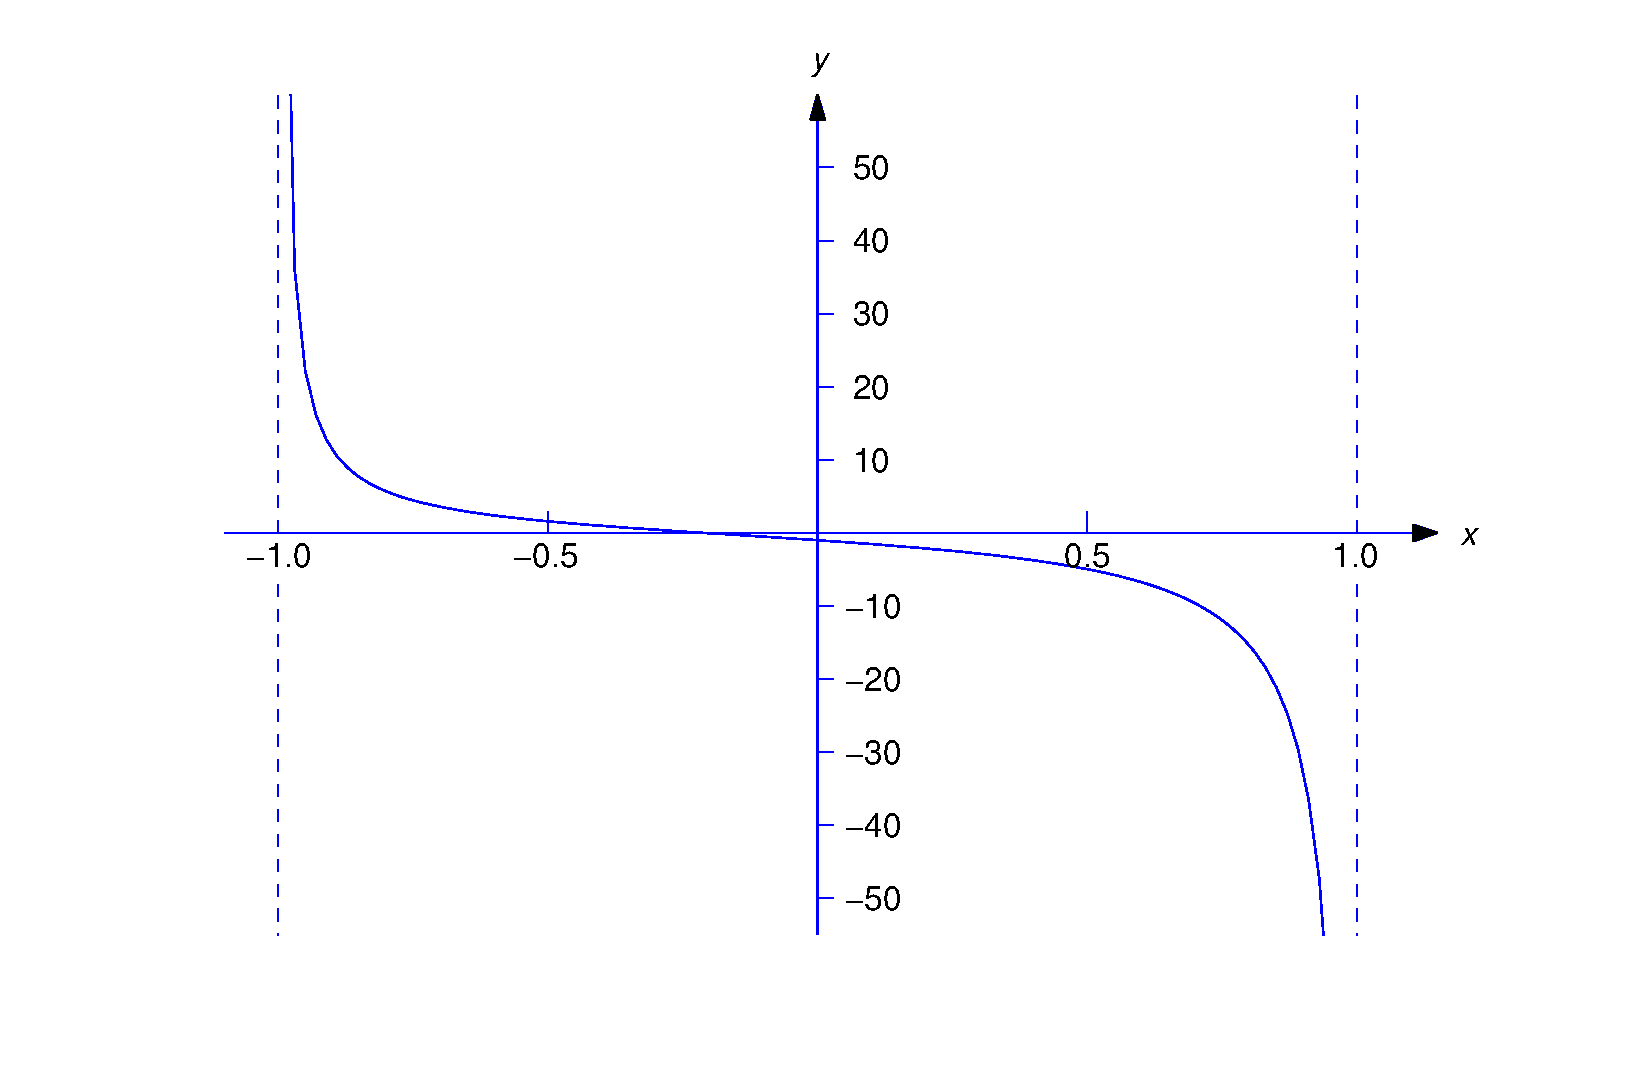
\includegraphics[bb=-78 148 689 643,width=5.67in,height=3.66in,keepaspectratio]{fig050701}
\color{blue}
  \caption{ $y=\dst{2\ln(x+1)\over x-1}+{3x+1\over x^2-1}$}
  \label{figure:5.7.1}
\end{figure}

\boxit{Comparison of Methods}

\noindent
We've now considered three methods
for solving  nonhomogeneous linear equations: undetermined
coefficients, reduction of order, and variation of parameters. It's
natural to ask which method is best for a given problem. The method of
undetermined coefficients should be used for constant coefficient
equations with forcing functions that are linear combinations of
polynomials multiplied by functions of the form $e^{\alpha x}$,
$e^{\lambda x}\cos \omega x$, or $e^{\lambda x}\sin \omega x$.
Although the other two methods can be used to solve such problems,
they will be more difficult except in the most trivial cases, because
of the integrations involved.

If the equation isn't  a constant coefficient equation or the forcing
function isn't  of the form just specified,  the method of
undetermined coefficients does not apply and the choice is necessarily
between the other two methods. The case could be made that reduction
of order is better because it requires only one solution of the
complementary equation while variation of parameters requires two.
However, variation of parameters will probably be easier if you
already know a fundamental set of solutions of the complementary
equation.

\exercises
 In Exercises~\ref{exer:5.7.1}--\ref{exer:5.7.6} use variation of
parameters to find a particular solution.

\begin{exerciselist}

\begin{tabular}[t]{@{}p{168pt}@{}p{168pt}}
\item\label{exer:5.7.1} $y''+9y=\tan 3x$
&\vspace*{10pt}  \item\label{exer:5.7.2} $y''+4y=\sin 2x\sec^2 2x$
\end{tabular}

\begin{tabular}[t]{@{}p{168pt}@{}p{168pt}}
\item\label{exer:5.7.3}  $y''-3y'+2y=\dst{4\over 1+e^{-x}}$
&  \item\label{exer:5.7.4} $y''-2y'+2y=3e^x \sec x$
\end{tabular}

\begin{tabular}[t]{@{}p{168pt}@{}p{168pt}}
\item\label{exer:5.7.5} $y''-2y'+y=14x^{3/2}e^x$
&\vspace*{-5pt} \item\label{exer:5.7.6} $y''-y=\dst{4e^{-x}\over
1-e^{-2x}}$
\end{tabular}
\newpage

\exercisetext{In Exercises \ref{exer:5.7.7}--\ref{exer:5.7.29} use variation
of parameters to find a particular solution, given the solutions
$y_1$, $y_2$ of the complementary equation.}

\item\label{exer:5.7.7}
$x^2y''+xy'- y=2x^2+2;   \quad y_1=x,
\quad y_2=\dst{1\over x}$

\item\label{exer:5.7.8}
$\dst{xy''+(2-2x)y'+(x-2)y=e^{2x};   \quad y_1=e^x,
\quad y_2={e^x\over x}}$

\item\label{exer:5.7.9}
$4x^2y''+(4x-8x^2)y'+(4x^2-4x-1)y=4x^{1/2}e^x, \quad   x > 0$;
\newline $y_1=x^{1/2} e^x,\;  y_2=x^{-1/2}e^x$

\item\label{exer:5.7.10}
$y''+4xy'+(4x^2+2)y=4e^{-x(x+2)};\quad   y_1=e^{-x^2},
\quad y_2=xe^{-x^2}$

\item\label{exer:5.7.11}
$x^2y''-4xy'+6y=x^{5/2},\, x > 0;\quad  y_1=x^2,\;  y_2=x^3$

\item\label{exer:5.7.12}
$x^2y''-3xy'+3y=2x^4\sin x; \quad  y_1=x,\;  y_2=x^3$

\item\label{exer:5.7.13}
$(2x+1)y''-2y'-(2x+3)y=(2x+1)^2e^{-x}; \quad  y_1=e^{-x},
\quad y_2=xe^x$

\item\label{exer:5.7.14}
$4xy''+2y'+y=\sin\sqrt x; \quad  y_1=\cos\sqrt x,
\quad y_2=\sin\sqrt x$

\item\label{exer:5.7.15}
$xy''-(2x+2)y'+(x+2)y=6x^3e^x;\quad  y_1=e^x,\quad  y_2=x^3e^x$

\item\label{exer:5.7.16}
$x^2y''-(2a-1)xy'+a^2y=x^{a+1}; \quad  y_1=x^a,
\quad y_2=x^a \ln x$

\item\label{exer:5.7.17}
$x^2y''-2xy'+(x^2+2)y=x^3\cos x; \quad  y_1=x\cos x,
\quad y_2=x\sin x$

\item\label{exer:5.7.18}
$xy''-y'-4x^3y=8x^5;\quad  y_1=e^{x^2},\;  y_2=e^{-x^2}$

\item\label{exer:5.7.19}
$(\sin x)y''+(2\sin x-\cos x)y'+(\sin x-\cos x)y=e^{-x}; \quad
y_1=e^{-x},\quad y_2=e^{-x}\cos x$

\item\label{exer:5.7.20}
$4x^2y''-4xy'+(3-16x^2)y=8x^{5/2}; \quad  y_1=\sqrt xe^{2x},\;  y_2=\sqrt
xe^{-2x}$

\item\label{exer:5.7.21}
$ 4x^2y''-4xy'+(4x^2+3)y=x^{7/2}; \quad  y_1=\sqrt x\sin x,\;
y_2=\sqrt x\cos x$

\item\label{exer:5.7.22}
$x^2y''-2xy'-(x^2-2)y=3x^4;\quad  y_1=xe^x,\;  y_2=xe^{-x}$

\item\label{exer:5.7.23}
$x^2y''-2x(x+1)y' +(x^2+2x+2)y=x^3e^x;   \quad y_1=xe^x, \quad y_2=x^2e^x$

\item\label{exer:5.7.24}
$x^2y''-xy'-3y=x^{3/2};  \quad y_1=1/x, \quad y_2=x^3$

\item\label{exer:5.7.25}
$x^2y''-x(x+4)y'+2(x+3)y=x^4e^x;  \quad y_1=x^2, \quad y_2=x^2e^x$

\item\label{exer:5.7.26}
$x^2y''-2x(x+2)y'+(x^2+4x+6)y=2xe^x;  \quad y_1=x^2e^x, \quad y_2=x^3e^x$

\item\label{exer:5.7.27}
$x^2y''-4xy'+(x^2+6)y=x^4;  \quad y_1=x^2\cos x, \quad y_2=x^2\sin x$

\item\label{exer:5.7.28}
 $(x-1)y''-xy'+y=2(x-1)^2e^x;  \quad y_1=x, \quad y_2=e^x$

\item\label{exer:5.7.29}
$4x^2y''-4x(x+1)y'+(2x+3)y=x^{5/2}e^x;   \quad
y_1=\sqrt x, \quad y_2=\sqrt xe^x$

\exercisetext{In Exercises \ref{exer:5.7.30}--\ref{exer:5.7.32} use variation
of parameters to solve the initial value problem, given
$y_1$, $y_2$ are solutions of the complementary equation.}

\item\label{exer:5.7.30}
$(3x-1)y''-(3x+2)y'-(6x-8)y=(3x-1)^2e^{2x}, \quad   y(0)=1,\;
y'(0)=2$;

$y_1=e^{2x},\;  y_2=xe^{-x}$

\item\label{exer:5.7.31}
$(x-1)^2y''-2(x-1)y'+2y=(x-1)^2, \quad   y(0)=3,\quad   y'(0)=-6$;

$y_1=x-1$,\;
$y_2=x^2-1$

\item\label{exer:5.7.32}
$(x-1)^2y''-(x^2-1)y'+(x+1)y=(x-1)^3e^x, \quad  y(0)=4,\quad y'(0)=-6$;

$y_1=(x-1)e^x,\quad y_2=x-1$

\newpage

\exercisetext{In Exercises \ref{exer:5.7.33}--\ref{exer:5.7.35} use variation
of parameters to solve the initial value problem and graph the
solution, given that $y_1$, $y_2$ are solutions of the complementary
equation.}

\item\label{exer:5.7.33} \CGex
$\dst{(x^2-1)y''+4xy'+2y=2x, \quad   y(0)=0,\;  y'(0)
=-2; \quad   y_1={1\over x-1},\;  y_2={1\over x+1}}$

\item\label{exer:5.7.34} \CGex
$\dst{x^2y''+2xy'-2y=-2x^2, \quad   y(1)=1,\;  y'(1)=
-1; \quad  y_1=x,\;  y_2={1\over x^2}}$

\item\label{exer:5.7.35} \CGex
$(x+1)(2x+3)y''+2(x+2)y'-2y=(2x+3)^2, \quad  y(0)=0,\quad y'(0)=0$;
\newline $y_1=x+2,\quad y_2=\dst{1\over x+1}$

\item\label{exer:5.7.36}
Suppose
$$
y_p=\overline y+a_1y_1+a_2y_2
$$
is a particular solution of
$$
P_0(x)y''+P_1(x)y'+P_2(x)y=F(x),
\eqno{\rm (A)}
$$
where  $y_1$  and $y_2$ are  solutions of the complementary equation
$$
P_0(x)y''+P_1(x)y'+P_2(x)y=0.
$$
Show that $\overline y$  is also a solution of  (A).

\item\label{exer:5.7.37}
Suppose $p$,  $q$, and $f$ are continuous
on $(a,b)$ and let $x_0$ be in $(a,b)$. Let
$y_1$ and $y_2$ be the  solutions of
$$
y''+p(x)y'+q(x)y=0
$$
such that
$$
y_1(x_0)=1, \quad y_1'(x_0)=0, \quad y_2(x_0)=0, \quad
y_2'(x_0)=1.
$$
Use variation of parameters to show that the solution of the initial
value problem
$$
y''+p(x)y'+q(x)y=f(x), \quad   y(x_0)=k_0,\;  y'(x_0)=k_1,
$$
is
$$
\begin{array}{rcl}
y(x) &=& k_0y_1(x)+k_1y_2(x) \\
& & \dst \qquad+\int^x_{x_0}\left(y_1(t)y_2(x)-
y_1(x)y_2(t)\right)
f(t)\exp\left(\int^t_{x_0}p(s)\,ds\right)\,dt.
\end{array}
$$
\hint{Use Abel's formula for the Wronskian of $\{y_1,y_2\}$, and
integrate $u_1'$ and $u_2'$ from $x_0$ to $x$.} Show also that
$$
\begin{array}{rcl}
y'(x) &=& k_0y_1'(x)+k_1y_2'(x) \\[2\jot]
& & \dst \qquad+\int^x_{x_0}\left(y_1(t)y_2'(x)-y_1'(x)y_2(t)
\right)f(t)\exp\left(\int^t_{x_0}p(s)\,ds\right)\,dt.
\end{array}
$$

\item\label{exer:5.7.38}
Suppose $f$ is continuous on an open interval
that contains $x_0=0$.
Use variation of parameters to
find a formula for the solution of the initial value problem
$$
y''-y=f(x), \quad  y(0)=k_0,\quad y'(0)=k_1.
$$

\item\label{exer:5.7.39}
Suppose $f$ is continuous on
$(a,\infty)$, where $a<0$, so $x_0=0$ is in $(a,\infty)$.

\begin{alist}
\item % (a)
Use variation of parameters to
find a formula for the solution of the initial value problem
$$
y''+y=f(x), \quad  y(0)=k_0,\quad y'(0)=k_1.
$$
\hint{You will need the addition formulas for the sine and cosine:
\begin{eqnarray*}
\sin(A+B)&=&\sin A\cos B+\cos A\sin B\\
\cos(A+B)&=&\cos A\cos B-\sin A\sin B.
\end{eqnarray*}}
\end{alist}

For the rest of this exercise assume that the improper
integral
$\int_{0}^\infty f(t)\,dt$ is absolutely convergent.

\begin{alist}[start=2]
\item % (b)
Show that if $y$ is a solution of
$$
y''+y=f(x)
\eqno{\rm (A)}
$$
 on $(a,\infty)$, then
 $$
\lim_{x \to \infty}\left(y(x)-A_0\cos x-A_1\sin x\right)=0
\eqno{\rm (B)}
$$
and
$$
\lim_{x\to\infty}\left(y'(x)+A_0\sin x-A_1\cos x\right)=0,
\eqno{\rm (C)}
$$
where
$$
A_0=k_0-\int_0^\infty f(t)\sin t\,dt\mbox{\quad and \quad}
A_1=k_1+\int_0^\infty f(t)\cos t\,dt.
$$
\hint{Recall from calculus that if $\int_0^\infty f(t)\,dt$
converges absolutely, then $\lim_{x\to\infty}\int_x^\infty
|f(t)|\,dt~=~0$.}

\item % (c)
Show that if $A_0$ and $A_1$ are arbitrary constants, then there's a
unique solution of $y''+y=f(x)$ on $(a,\infty)$ that satisfies
(B)  and (C).
\end{alist}

\end{exerciselist}


